\documentclass[a4paper, openright, twoside]{report}
\usepackage[utf8]{inputenc}
\usepackage[main=american, german]{babel}
\usepackage{hyphenat}
\usepackage[activate={true,nocompatibility}, final, tracking=true, kerning=true, factor=1100, stretch=10, shrink=10]{microtype}
% Prevent hyphenization
\tolerance=1
\emergencystretch=\maxdimen
\hyphenpenalty=10000
\hbadness=10000

\usepackage[hmarginratio=1:1,textwidth=360pt,textheight=595.8pt]{geometry}
% Packages
\usepackage{import}

% Math
\newcommand\hmmax{0}
\newcommand\bmmax{0}
\usepackage{bm}
\usepackage{amsmath, amsfonts, amssymb, mathrsfs,extarrows}
\usepackage{upgreek}
\usepackage{commath}
\usepackage[retainorgcmds]{IEEEtrantools}
\usepackage{siunitx}
\sisetup{%
  print-unity-mantissa=false,
  % exponent-mode=engineering,
  range-phrase = {\ \linebreak[0]\text{to}\ \nolinebreak},
  list-separator = {\text{, }},
  list-final-separator = {,\ \linebreak[0]\text{and }},
  list-pair-separator = {\ \text{and}\ },
  list-separator = {,\ \linebreak[0]}
  }%
\usepackage{multirow}
\usepackage[widespace]{fourier}

% Tables
\usepackage{array}
\usepackage{caption}
\usepackage[figuresright]{rotating}
\usepackage{multirow}
\usepackage{makecell}
\usepackage{footnote}
\usepackage{booktabs}
\usepackage{lscape}
\makesavenoteenv{tabular}

% Algorithm
\usepackage[chapter]{algorithm}
\usepackage{algpseudocode}

%% Citations
\usepackage[numbers]{natbib}
\bibliographystyle{plainnat}
\citestyle{egu}
\usepackage[hyphens]{url}
% Bibliography showing in TOC
% \usepackage[nottoc,numbib]{tocbibind}
\usepackage[nottoc]{tocbibind}
\usepackage{scrlayer}
\DeclareNewLayer[
    foreground,
    %textarea,% use only the textarea
    contents={%
      \parbox[b][\layerheight][c]{\layerwidth}
        {\centering Page intentionally left blank.}%
    }
  ]{blankpage.fg}
\DeclarePageStyleByLayers{blank}{blankpage.fg}

% Control structures
\usepackage{ifthen}

% Listing
\usepackage{listings}
\usepackage[table,dvipsnames]{xcolor}
\usepackage{float}

% Review notes:
\usepackage{xargs}
\usepackage[textwidth=30mm,textsize=footnotesize]{todonotes} % to create comments (useful to your advisor!)
\newcommandx{\bpf}[2][1=]{\todo[linecolor=blue,backgroundcolor=blue!25,bordercolor=blue,#1]{#2}} % Bernardo notes
\newcommandx{\jvc}[2][1=]{\todo[linecolor=orange,backgroundcolor=orange!25,bordercolor=orange,#1]{#2}} % My notes

% Equation color background
\usepackage{mdframed}

\newmdenv[
    hidealllines=true,
    backgroundcolor=black!20,
    skipbelow=\baselineskip,
    skipabove=\baselineskip
]{highlight}

\newcounter{problem}[chapter]\setcounter{problem}{1}
\renewcommand{\theproblem}{\arabic{chapter}.\arabic{problem}}
\newenvironment{problem}[2][]{%
    \refstepcounter{problem}

    \mdfsetup{hidealllines=true,
    backgroundcolor=black!20,
    skipbelow=\baselineskip,
    skipabove=\baselineskip,
    frametitle={Problem~\theproblem~|~#1}}

\begin{mdframed}[]\relax}{%
\end{mdframed}}

\newcounter{remark}[chapter]\setcounter{remark}{1}
\renewcommand{\theremark}{\arabic{chapter}.\arabic{remark}}
\newenvironment{remark}[2][]{%
    \refstepcounter{remark}

    \mdfsetup{hidealllines=true,
    backgroundcolor=black!20,
    skipbelow=\baselineskip,
    skipabove=\baselineskip,
    frametitle={Remark~\theremark~|~#1}}

\begin{mdframed}[]\relax}{%
\end{mdframed}}

% Enumeration
\usepackage{enumerate}


% Images
\usepackage[labelformat=simple]{subcaption}
\renewcommand\thesubfigure{(\alph{subfigure})}
\renewcommand\thesubtable{(\alph{subtable})}
\usepackage{graphicx}
\graphicspath{ {figures/} }
\usepackage{array}
\usepackage[section]{placeins}
\usepackage{color}
% \usepackage{subcaption}
% \usepackage{subfig}



% Images SVG
\usepackage{import}
\usepackage{xifthen}
\usepackage{pdfpages}
\usepackage{transparent}

\newcommand{\incfig}[1]{
    \def\svgwidth{0.3\columnwidth}
    \import{images/studies/minkowski/fundamental_forms_2D/}{#1.pdf_tex}}


% Floating environment for listings
\floatstyle{plain}
\newfloat{lstfloat}{htbp}{lop}[chapter]
\floatname{lstfloat}{Listing}
\def\lstfloatautorefname{Listing} % needed for hyperref/auroref

% Listing style
\definecolor{codegreen}{rgb}{0,0.6,0}
\definecolor{codegray}{rgb}{0.5,0.5,0.5}
\definecolor{codepurple}{rgb}{0.58,0,0.82}
\definecolor{backcolour}{rgb}{0.95,0.95,0.92}

\lstdefinestyle{mystyle}{
    backgroundcolor=\color{backcolour},
    commentstyle=\color{codegreen},
    keywordstyle=\color{blue},
    numberstyle=\tiny\color{codegray},
    stringstyle=\color{codepurple},
    basicstyle=\fontsize{7}{10}\selectfont,
    breakatwhitespace=false,
    breaklines=false,
    captionpos=b,
    keepspaces=true,
    numbers=left,
    numbersep=5pt,
    showspaces=false,
    showstringspaces=false,
    showtabs=false,
    tabsize=2
}

\lstset{style=mystyle}

\makeatletter
\newcommand*{\shifttext}[2]{%
  \settowidth{\@tempdima}{#2}%
  \makebox[\@tempdima]{\hspace*{#1}#2}%
}
\makeatother

\usepackage{pythonhighlight}

% Appendices
\usepackage[toc,page]{appendix}

% Headers and footers
\usepackage{fancyhdr}
% \renewcommand{\chaptermark}[1]{\markboth{\thechapter.\ #1}{}}
% \renewcommand{\sectionmark}[1]{\markright{\thesection.\ #1}}

% \fancypagestyle{plain}{
% \fancyhf{}
% \fancyhead{}% remove default header entries
% \fancyhead[RE]{a\textsc{\leftmark}}
% \fancyhead[LE]{\thepage}
% \fancyhead[LO]{\textsc{\rightmark}}
% \fancyhead[RO]{\thepage}
% \renewcommand{\headrulewidth}{0.1pt} }
% \pagestyle{plain}

\fancypagestyle{firststyle}
{
   \fancyhf{}
    \fancyhead{}% remove default header entries
   \fancyfoot[C]{Porto, July 2022}
   \renewcommand{\headrulewidth}{0pt}
\renewcommand{\footrulewidth}{0.1pt}
    \fancyfootoffset{-0.25\textwidth}
}

\pagestyle{fancy}
\fancyhf{}
\renewcommand{\chaptermark}[1]{\markboth{\thechapter.\ #1}{}}
\renewcommand{\sectionmark}[1]{\markright{\thesection.\ #1}}
\fancyhead{}% remove default header entries
\fancyhead[RE]{\nouppercase\leftmark}
\fancyhead[LE]{\thepage}
\fancyhead[LO]{\nouppercase\rightmark}
\fancyhead[RO]{\thepage}
\renewcommand{\headrulewidth}{0.1pt}

\newenvironment{dedication}
  {%\clearpage           % we want a new page          %% I commented this
   \thispagestyle{empty}% no header and footer
   \vspace*{\stretch{1}}% some space at the top
   \itshape             % the text is in italics
   \raggedleft          % flush to the right margin
  }
  {\par % end the paragraph
   \vspace{\stretch{3}} % space at bottom is three times that at the top
   \clearpage           % finish off the page
  }


% landscape
% \usepackage{lscape}
\usepackage{pdflscape}

%Custom FramedBox Environment
%%Loading 'float' package
\usepackage{float}
%%Customize 'boxed' float style (caption above the body)
\makeatletter
\newcommand\fs@boxedtop
 {\fs@boxed
  \def\@fs@mid{\vspace\abovecaptionskip\relax}%
  \let\@fs@iftopcapt\iftrue
 }
\makeatother
%%Defining float commands
\floatstyle{boxedtop}
\floatname{framedbox}{Box}
\newfloat{framedbox}{hbt}{lob}[chapter]

% Symbols
%% Differential Upright "d"
\newcommand{\ud}{\,\mathrm{d}}
%% Assemble operator
\DeclareMathOperator*{\assemble}{\text{\Large $ \mathsf{A} $}}
%% Matrices and vectors
\newcommand{\vect}[1]{\bm{#1}}
\newcommand{\mat}[1]{\bm{#1}}
\newcommand{\boldsf}[1]{\boldsymbol{\mathsf{#1}}}

\DeclareMathAlphabet{\pazocal}{OMS}{zplm}{m}{n}

\title{Thermomechanial modeling of semi-crystalline polymers}
\author{José Luís Passos Vila-Chã}
\date{February 2023}


\pagenumbering{roman}

%Hypertext marks
\usepackage[pdftitle={PRODEM_seminar},
			pdfauthor={JoseVila-Cha},
			pdfdisplaydoctitle=true,
			colorlinks=true,
			% Eletronic Version
             linkcolor=orange,
             citecolor=teal,
            % Print Version
            % linkcolor=black,
            % citecolor=black,
            bookmarks=true,
            bookmarksopen=false,
            bookmarksnumbered=true]{hyperref}

\usepackage[intoc]{nomencl}
\usepackage{xstring}
\usepackage{xpatch}
\patchcmd{\thenomenclature}
  {\leftmargin\labelwidth}
  {\leftmargin\labelwidth\itemindent 1em }
  {}{}

% Nomenclature

\makenomenclature
\renewcommand{\nomname}{Notation}
%% This code creates the groups
% -----------------------------------------
\usepackage{etoolbox}
\newcommand{\nomenclheader}[1]{%
  \item[\hspace*{-\itemindent}\bfseries\LARGE#1\vphantom{$\Bigg \vert $}]}
\renewcommand\nomgroup[1]{%
  \IfStrEqCase{#1}{%
   {A}{\nomenclheader{General abbreviations}}%      A - Acronyms
   {N}{\nomenclheader{General notation}}% R - Roman
   {O}{\nomenclheader{Operators and symbols}}% G - Greek
   {D}{\nomenclheader{Sets, domains and boundaries}}% G - Greek
   {S}{\nomenclheader{Subscripts and superscripts}}%  S - Superscripts
   {C}{\nomenclheader{Accents}}%    U - Subscripts
   {V}{\nomenclheader{Variables}}% X - Other Symbols
  }%
  \vspace{20pt}
}
\setlength{\nomitemsep}{-1pt}
% -----------------------------------------

\begin{document}
\begin{titlepage}
\thispagestyle{firststyle}
\begin{center}
   \begin{minipage}[c][10cm][l]{0.9\textwidth}

        
\includegraphics[width=0.6\textwidth]{figures/university}

        \vspace{3.5cm}
        \huge
       \textbf{Thermomechanical modeling of semi-crystalline polymers}

       \vspace{1.5cm}
        \small
       \textit{Professor:}\\
       \normalsize
       Renato Manuel Natal Jorge 	 	\\

       \vspace{0.5cm}


         \small
        \textit{Student:}\\
        \vspace{0.5cm}
       \normalsize
       \!José Luís Passos Vila-Chã
       \vspace{7.5cm}


        \centering
        \small
       Report presented under the scope of the\\ Doctoral Program in Mechanical Engineering

   \end{minipage}
   \end{center}
\end{titlepage}

\newpage\null\thispagestyle{blank}\newpage

\setcounter{tocdepth}{3}
\setcounter{secnumdepth}{3}
\tableofcontents


\listoffigures
\newpage\null\thispagestyle{blank}\newpage

\listoftables
\newpage\null\thispagestyle{blank}\newpage

\pagenumbering{gobble}
\pagenumbering{arabic}
\pagestyle{fancy}
\chapter{Introduction}

\section{Context}

Design permeates engineering.
Ashby \citep{ashbyMaterialsSelectionMechanical1999} identifies the main features of mechanical design as being:
\begin{itemize}
    \item function;
    \item material;
    \item shape;
    \item and process.
\end{itemize}
There is a profound interplay between all these facets of design when developing a mechanical component.
Accordingly, the component must meet functional criteria in terms of its thermomechanical behavior.
Additional specifications of its electric, magnetic, or mass transfer characteristics may also be prescribed.
The aptitude of said component to satisfy these demands will be determined by the material or materials from which it is made, as well as its shape.
Some materials, however, cannot be manufactured into a particular shape or at all using a specific manufacturing process.
Weight, cost, and environmental impact reduction can all be included as goals, and their achievement is closely related to the material and method selected.

An even more intimate relationship between the final performance of the mechanical component and the process selected for its manufacturing may be uncovered taking into account the hierachical structure of engineering materials.
Accordingly, Olson \citep{olsonDesigningNewMaterial2000} emphasizes the cause/effect relationship between the process, the material's structure at multiple scales ranging from the nanoscale to the macroscale, the material's properties, and its final performance.
The reverse goals/means perspective can also be adopted where a given performance requirement drives the search for a material with a given set of properties.
These in turn may only be realised if the appropriate multi-scale structure is obtained through a suitable process.
"Integrated Computational Materials Engineering" (ICME) is a systematic approach proposed by Horst \citep{horstemeyerCradletograveSimulationbasedDesign2003} that includes these relationships within a computational framework.
Its goal is the simulateneous design of a component, the materials that make them up and the manufacturing process employed, taking into account the material's structure at different scales.
To realize this vision, suitable models and numerical tools for simulating processes at a given time and length scale, as well as experimental methods to probe their validity and acquire material parameters in the model, must be available.
To accurately capture the behavior of the material, the correct boundary conditions, initial conditions, and material parameters must be established at each scale and time-frame.
An adequate way to transfer information between the different scales must also be devised.

Taking into account the hierarchial nature of a material's structure, appropriate models must be set up at the structural (meters, centimeters), macro (millimeters), meso (hundred to tenths of micrometers), micro (micrometers) and atomic/nanoscale (angston).
Relevant to this work is the strcutrual scale, where solutions from FEM are used to model both the manufacturing and the product life.
Full scale experiments are employed to gauge the accuracy of the predictions.
At the macroscale an appropriate constitutive/rheological model must be devised.
Its use in an appropriate FEM simulation and comparison with simple mechanical experiments, e.g., unixial or torsion experiments, is used for validation.
Retaining the appropriate continuum constitutive models and including an accurate representation of a polymer blend at the mesoscale may allow its constitutive description.

\section{Motivation}

The current work focuses on two aspects of the aforementioned paradigm: the use of FEM in the structural response of a component to solve multi-physics problems, particularly those involving thermomechanical phenomena, and the macroscale constitutive description of semi-crystalline polymers.

\subsection{Multi-physics simulations}

It is generally understood that thermomechanics is a crucial physical phenomenon in engineering applications and a highly sought-after feature in computational models.
These effects play a central role in mainstream and heavy-duty thermomechanical applications such as rocket nozzles \citep{kuhl2002ThermomechanicalAnalysisOptimization,danowski_monolithic_2013}, disk brakes and clutches \citep{yevtushenko2015NumericalAnalysisThermal}, heat-assisted incremental sheet forming \citep{liu2018HeatassistedIncrementalSheet} and thermal stresses due to machining \citep{elsheikh2021ComprehensiveReviewResidual}, for instance.
There is a profound interplay between the mechanical and the thermal field:
\begin{\itemize}
  \item the thermal field influences the mechanical through temperature-dependent properties and the appearance
\end{\itemize}

Give examples of applications thermomechanics and thermomechanics electric and so on.

To include a solver for the thermomechanical problem in a numerical simulation toolbox, the problem has to be correctly formulated in a thermodynamically consistent way.
Having achieved an appropriate formulation of the problem, the Finite Element Method can be used to solve it.
After the spatial discretization obtained by the FEM has been provided, the complete thermomechanical problem can still be solved by employing two different strategies: a monolithic approach or a partitioned approach.
In the former, the discretized equations representing the momentum balance and energy conservation are solved simultaneously.
In the latter, the problems are solved independently, solving the mechanical problem at a fixed temperature and then the thermal problem at a fixed configuration, taking the so-called isothermal split as an example.
With this last scheme, one can still find the loosely or explicit approaches and the strongly coupled or implicit approaches as alternatives.
Each of these strategies has its benefits and drawbacks, with the particular choice of one over the others depending on the particulars of the development environment.

\subsection{Semi-crystalline polymers}

Semi-crystalline polymers have a complex and hierarchial heterogeneous morphology.
Both their microstructure and their mesostructure will depend on the processing history, as well as mechanical and thermal histories, in addition to the polymer chemistry and conformation \citep{khouryMorphologyCrystallineSynthetic1976,cangemiTwoPhaseModelMechanical2001,hoffmanAnalysisRelaxationsPolychlorotrifluoroethylene2007}.

Why polymers good.

\paragraph{Examples and applications}

Employ all props for comparison with metals, ceramics and composites.

stiff and yield vs densitiy. Polymer best if low weight is benefit.

Polymer not as though

Polymers best at strain failure.

 Manufacturing.

\paragraph{Microstructure}
At the microscopic level, they consist of at least two different phases: a crystalline phase and an amorphous phase \citep{khouryMorphologyCrystallineSynthetic1976}.
The ordered structure that composes the crystalline portion of a semi-crystalline polymer results from the constituent chains packing parallel to one another in an orderly fashion into lamellae, as show in Figure~\eqref{fig:crystalline_phase_of_scp}.

\begin{figure}[htbp]
	\includegraphics[width=0.9\textwidth]{example-image-a}
	\caption{Arrangement of polymer chains into a lamella in the crystalline phase of a semi-crystalline polymer.}
\label{fig:crystalline_phase_of_scp}
\end{figure}

There are at least two types of crystal lamellae found in semi-crystalline polymers, as detailed in \cite{andersonMorphologyIsothermallyBulk1964} for polyethylene (PE), the  chain-folded lamellae and extended-chain lamellae (see Figure~\eqref{fig:types_of_crystall}).
In the former, the molecular chains within each platelet fold back and forth on themselves, with folds occurring at the faces.
This is in fact, an idealization, with reality resembling more a switchboard model, with the chains reentering through loose folds at non-adjacent sites or even forming tie-chains with a neighboring lamellae \citep{gsellEvolutionMicrostructureSemicrystalline1994}.
The latter is more common at lower molecular weights with the chains organized into lamellae in their extended conformation.
The thickness of the lamellae in semi-crystalline polymers is of the order of nanometers, e.g., between \SIrange{10}{15}{\nano\meter} for PE samples \citep{argonPhysicsDeformationFracture2013a}.
\begin{figure}[hbtp]
	\includegraphics{example-image-a}
	\caption{Schematic depictions of chain-folded and extended-chain lamellae.}
\label{fig:types_of_crystall}
\end{figure}

Regarding the crystalline structure, it will depend on the polymer in question.
PE possesses most often an orthorhombic symmetry, where the chain direction forms an angle with the normal vector to the crystalline lamella ranging between 17 and $40^\circ$ \citep{nikolovMicroMacroConstitutive2000}.
On the other hand, the crystal structure found in polytetrafluoroethylene (PTFE) at temperatures above \SI{19}{\celsius} is hexagonal, with individual molecules arranged in helical conformations \citep{bergstromMechanicsSolidPolymers2015}.
See Figure~\ref{fig:crystalline_structure_PE_PTFE} for a depiction of both crystalline structures.
\begin{figure}[hbtp]
	\includegraphics[width=0.9\textwidth]{example-image-a}
	\caption{Depiction of the crystalline structures of polyethylene (PE) and polytetrafluoroethylene (PTFE).}
\label{fig:crystalline_structure_PE_PTFE}
\end{figure}

The crystallinity of a semi-crystalline polymer can be specified by the degree of crystallinity.
It may range from completely amorphous to almost entirely crystalline.
\cite{wardIntroductionMechanicalProperties2004} mentions values between $90\%$ for polyethylene (PE) to about $30\%$ for oriented poly(ethylene terephthalate) (PET).
Commercially available semi-crystalline polymers range from $10\%$ to $90\%$ in degree of crystallinity \citep{vandommelenMicromechanicalModelingElastoviscoplastic2003}.

The degree of crystallinity by weight may be determined from accurate density measurements, according to
\begin{equation}
	\chi = \% \text { crystallinity }=\frac{\left(\rho_{s}-\rho_{a}\right)/\rho_{s}}{\left(\rho_{c}-\rho_{a}\right)/\rho_{c}} \times 100
\end{equation}
where $\rho_{s}$ is the density of a specimen for which the percent crystallinity is to be determined, $\rho_{a}$ is the density of the totally amorphous polymer, and $\rho_{c}$ is the density of the perfectly polymer crystallite.
The values of $\rho_{a}$ and $\rho_{c}$ must be measured by other experimental means.
Other experimental methods employed to determine the crystallinity along with the lamellar thickness of the polymer crystallites include wide (WAXS) and small (SAXS) angle X-ray scattering \citep{schrauwenIntrinsicDeformationBehavior2004, hobeikaTemperatureStrainRate2000}, as well as, electron microscopic, e.g., transmission electron microscopy (TEM) \citep{bartczakEvolutionCrystallineTexture1992}.

The parameters influencing the crystallinity are mainly the molecular structure, the molecular weight, the presence of plasticizers, and especially the thermo-mechanical history of the polymer \citep{khouryMorphologyCrystallineSynthetic1976, cangemiTwoPhaseModelMechanical2001}.
Given the way that polymer crystals form, polymer chains must possess a linear structure.
The more branches/pendant side groups the lesser the degree of crystallinity.
Even linear polymers must, however, have sufficient regularity in order to crystallize \citep{khouryMorphologyCrystallineSynthetic1976}.
A high molecular weight tends to suppress a high degree of crystallinity \citep{hoffmanAnalysisRelaxationsPolychlorotrifluoroethylene2007}, as seen comparing high density polyethylene (HDPE) and ultra high weight polyethylene (UHWPE) \citep{brownInfluenceMolecularConformation2007}.
Given that the crystallization is a kinetic process the rate of crystallization in polymers is dependent on the temperature with larger temperatures leading to smaller rates \citep{callister2014materials}.
As detailed later in this chapter, the mechanical loading of a polymer may also lead to changes in its crystallinity, e.g., through the phenomenon of strain-induced crystallization \citep{raoStudyStraininducedCrystallization2001}.

Accordingly, the most frequent approach to achieve different degrees of crystallinity is through the control of crystallization temperatures and/or crystallization times, be it when crystallizing from the melt or through annealing treatments \citep{fakirovGlassTransitionTemperature2000, schrauwenIntrinsicDeformationBehavior2004}.
However, the preparation of samples with different degrees of crystallinity is not a routine task for polymers such as HDPE, since its rate of crystallization is very high.
One solution is to take PE samples differing in the degree of branching, since by introducing various amounts of defects in the main chain, it is possible to control the degree of crystallinity \citep{fakirovGlassTransitionTemperature2000}.

In what pertains to the amorphous portion of a semi-crystalline polymer, results reported by Zia et al. \citep{ziaRigidAmorphousFraction2008} on isotactic polypropylene (iPP), for example, point to the existence of two different amorphous phases, a mobile amorphous phase and rigid amorphous phase, on the basis of different glass transition temperatures.
The results of Jolly \citep{jollyAnalyseMicrostructurePolyamide2000} concerning polyamide 11 (PA11) found employing WASX, carried out at different axial deformation rates also support the existence of a neither pure amorphous nor crystalline phase.
According to Mandelkern \citep{mandelkernCrystallinePolymerReminiscences2006}, the existence of a rigid amorphous phase is supported by experimental experimental results obtained from density measurements, wide and small-angle X-ray diffraction, thermal analyses, Raman spectroscopy, small-angle neutron scattering, dielectric relaxation and nuclear magnetic resonance involving different nuclei and techniques.

The reason for the increased rigidity in this part of the amorphous phase is the presence of polymer crystallites, which hinder the molecular mobility of the amorphous phase \citep{ziaRigidAmorphousFraction2008, peacockHandbookPolyethyleneStructures2014}.
However, an increase in degree of crystallinity will lead to a decrease in the rigid amorphous fraction as well as the ratio between rigid and mobile amorphous phase.
This behavior is due to reduced covalent coupling between the polymer crystals and the amorphous phase in highly crystalline preparations\citep{ziaRigidAmorphousFraction2008}.
Furthermore, the presence of the crystallites also affects the properties of the mobile amorphous fraction, which is detected by a distinct decrease its glass transition temperature, as shown for semi-crystalline iPP by Zia et al. \citep{ziaRigidAmorphousFraction2008}.

\paragraph{Mesostructure}
According to the processing, thermal and mechanical history, as well as, its degree of crystallinity, molecular weight and polydispersity, a semi-crystalline polymer can display different mesoscopic structures \citep{cangemiTwoPhaseModelMechanical2001, mandelkernCrystallinePolymerReminiscences2006}.

When the polymer crystallizes from the a dilute solution the structure achieved is often lamellar and composed of multiple layers, if the solution is quiescent, and of the shish-kebab variety\footnote{The so-called shish-kebab structure consists of long central fiber core (shish) surrounded by lamellar crystalline structure (kebab) periodically attached along the shish.
\citep{naViscousForceDominatedTensileDeformation2006, peacockHandbookPolyethyleneStructures2014}.}, if the solution is subject to high shear \citep{khouryMorphologyCrystallineSynthetic1976, callister2014materials, peacockHandbookPolyethyleneStructures2014}.
When the polymer crystallizes from the melt, the two most commonly reported types of mesoscopic structures for semi-crystalline polymers are the spherulitic structure \citep{zengConstitutiveModelSemicrystalline2010}, obtained from quiescent crystallization, and the shish-kebab structure, obtained from crystallization under shear stress.
For a schematic depiction of a spherulitic and a shish-kebab structure see Figure~\ref{fig:mesostructure_scp}.
\begin{figure}[hbtp]
	\includegraphics[width=.9\textwidth]{example-image-a}
	\caption{Schematic depiction of a spherulitic and a shish-kebab mesostructure.}
\label{fig:mesostructure_scp}
\end{figure}

The spherulitic structure is composed of spherulites, an aggregate of ribbon-like chain-folded crystallites approximately 10 to \SI{20}{\nano\meter} thick for PE and 2 to \SI{6}{\nano\meter} for polyether ether ketone (PEEK), e.g., that radiate outward from a single nucleation site in the center, their diameter approximately \SI{10}{\micro\meter}.
Between them there are amorphous regions, crossed by tie-chain molecules that act as connecting links between adjacent lamellae \citep{callister2014materials, khouryMorphologyCrystallineSynthetic1976, pouriayevaliConstitutiveDescriptionRatesensitive2013, gsellEvolutionMicrostructureSemicrystalline1994}.
The lamellae are generally twisted about their long axis \citep{patlazhanStructuralMechanicsSemicrystalline2012}.
A sheave-like structure is also possible under suitable conditions \citep{peacockHandbookPolyethyleneStructures2014}.
Mandelkern \citep{mandelkernCrystallinePolymerReminiscences2006} warns however that spherulites, and other type of supermolecular structures, are not universally observed in homopolymers.

Mechanical loading will also lead to changes in the mesoscopic structure of the polymer.
Regarding higher crystallinity polymers such as HDPE, it normally results in the destruction of the crystallites of the original morphology, followed by reordering to form new crystallites.
The new lamellar morphology has a lamellar thickness independent of the original lamellar thickness, being solely dependent upon the temperature at which the deformation occurred .
In such morphologies the unit cell axes are preferentially aligned in the stress direction, while the lateral planes of the lamellae lie approximately normal to the aligning force.
These, newly formed crystallites are themselves subject to disruption at higher deformation levels (draw ratios of approximately 10), being replaced by a fibrillar morphology, which consists of oriented crystallites arranged hierarchically into needle-like structures of various sizes.
These macrofibrils are composed of microfibrils, in turn made up of nanofibrils, stacks of crystallites separated by thin noncrystalline “plates," portions of which are spanned by “intercrystalline bridges" \citep{peacockHandbookPolyethyleneStructures2014}.
A nearly perfect alignment of the crystallized chains along the fiber axis, as well as the parallel arrangement of the crystal lamellae relative to the same axis, define the final fiber structure \citep{peterlinMolecularModelDrawing1971}.
Moreover, plastically deforming HDPE develops three important types of texture, resembling that of a large quasi-single crystal \citep{argonPhysicsDeformationFracture2013a}:
\begin{enumerate}
	\item crystallographic texture due to preferential orientation of crystallographic axes in the crystalline lamellae;
	\item morphological texture due to preferential orientation of the normals to the broad faces of the crystalline lamellae faces; and
	\item macromolecular texture in the amorphous component, which is promoted by alignment of molecules with the direction of maximum stretch.
\end{enumerate}

At the other extreme, for materials such as PET, in which the crystalline and amorphous components are intermixed, the most noticeable effect may be strain-induced crystallization due to macromolecular texture as described above \citep{wardIntroductionMechanicalProperties2004}.
More specifically, temperatures above the glass transition temperature, a linear structure and large deformations lead to an increase in the crystallinity of the material \citep{ahziModelingDeformationBehavior2003}.
The crystalline structures produced in this way are oriented, which results in an anisotropic mechanical response.
Experiments on polymer film also point to crystallization at lower strain when the strain rate is higher \citep{raoStudyStraininducedCrystallization2001}.
In fact,  a majority of plastic products are manufactured by deforming the material at elevated temperatures to get it into the desired shape.
Common examples of these types of operations include film blowing, fiber spinning and injection molding.
In many of these applications, the formation of a highly oriented crystalline phase has a beneficial impact on the mechanical behavior of the material \citep{dairaniehPhenomenologicalModelFlowInduced1999, raoStudyStraininducedCrystallization2001}.
Most PET articles are manufactured in this way \citep{boyceConstitutiveModelFinite2000, raoStudyStraininducedCrystallization2001, makradiTwophaseSelfconsistentModel2005}.


\section{Computational Framework}

All the numerical simulations based on the Finite Element Method (FEM) are held in the in-house Fortran (IBM Mathematical Formula Translation System) program LINKS (Large Strain Implicit Non-linear Analysis of Solids Linking Scales), a multi-scale finite element code for implicit infinitesimal and finite strain analyses of hyperelastic and elastoplastic solids, that is continuously developed by the CM2S research group (Computational Multi-Scale Modeling of Solids and Structures) at the Faculty of Engineering of University of Porto.

In the present work, the author contributes to the addition of a suitable coupling environment for the partitioned solution of coupled fields and a thermal solver based on the Finite Elements Method.
Appropriate nonlinear solvers are also added as implicit solution strategies for the coupled thermomechanical problem.

\section{Objectives}

The main goals of this work are:
\begin{itemize}
    \item To describe in a thermodynamically consistent way the thermomechanical problem;
    \item To develop and validate a thermal solver based on the Finite Element Method;
    \item To provide a thorough overview of the available methods for the solution of coupled problems, in particular, the thermomechanical problem;
    \item To validate the thermomechanical solver and compare the strongly coupled partitioned strategies available in the literature.
\end{itemize}

\section{Document structure}

The remainder of this document is structured as follows:

\paragraph{Chapter \ref{ch:thermomechanical_problem} - Continuum Thermomechanics}\mbox{}\\
This chapter covers the notions required to explain how a solid responds to thermal and mechanical loads under large deformations, including the conservation laws that guarantee mechanical equilibrium and energy conservation.
Additionally, the application of thermodynamics with internal variables is discussed, along with the resulting inferences about the constitutive behavior of the material that makes up the solid.

\paragraph{Chapter \ref{ch:thermomechanical_behavior_semi_crystalline_polymer} - Thermomechanical behavior of semi-crystalline polymers}\mbox{}\\
This chapter details the validation results for the thermal solver using as references the \cite{DINEN1991_1_2} and \cite{NAFEMSbenchmarks}.
It includes both transient effects and boundary conditions such as natural convection and radiation.

\paragraph{Chapter \ref{ch:modeling_semi_crystalline_polymer} - State of the art in thermomechanical semi-crystalline polymer modeling}\mbox{}\\
This chapter presents an overview of the solution procedures for coupled problems.
It includes monolithic schemes and partitioned schemes, both explicit and implicit approaches.
An evaluation and discussion of the different methods are provided.

\paragraph{Chapter \ref{ch:numerical_results} - Numerical results}\mbox{}\\
This chapter provides a thorough description of the available implicit methods.
It rests on recasting the problem as a simple root-finding problem for a set of nonlinear equations.
The methods presented are the fixed-point method, the underrelaxation method, the Aitken relaxation, the Broyden-like family of methods, the Newton-Krylov methods, and the polynomial vector extrapolation methods in cycling mode.
The number of residual evaluations, the memory requirements, the computational complexity, and the ease of implementation are all discussed for each approach.

\paragraph{Chapter \ref{ch:conclusions} - Conclusion and Future Works}\mbox{} \\
This chapter presents the conclusions reached in this work, and some future research directions are suggested.

\newpage\null\thispagestyle{blank}\newpage

\chapter{Thermomechanical problem} \label{sec:thermomechanical_problem}

This section provides a fundamental description of a solid material response when subject to both mechanical and thermal loads in a finite strain setting.
It also discusses the application of thermodynamics with internal variables, along with the resulting inferences about the constitutive behavior of the material that makes up the solid, setting up a suitable background for the remainder of the paper.

\section{Kinematics of deformation}

Let a deformable body $\mathscr{B}$ occupy an open region $\Omega_0$ of the tridimensional Euclidean space $\mathscr{E}$ with a regular boundary $\partial \Omega_0$ in its reference configuration.
A smooth one-to-one function defines its motion \(\bm{\varphi}\colon \Omega\times \mathbf{R}\to \mathscr{E}\), mapping each material particle of coordinates $\bm{X}$ in the reference configuration to its position $\bm{x}$ in the deformed configuration.
Accordingly, the displacement is defined as \(\bm{u}\equiv \bm{x} - \bm{X}\).
In this paper, the finite deformation of the body is described with respect to the initial configuration, following the so-called Lagrangian or material description.
Accordingly, the well-known deformation gradient second-order tensor is defined as \(\bm{F}(\bm{X},t)\equiv \nabla_0\bm\varphi(\bm{X},t)\), and its determinant, denoted as \(J\equiv \text{det}\;\bm{F} \geq 0\) represents the local unit volume change.

\section{Fundamental conservation principles} \label{sec:fundamental_conservation_princ}

In continuum thermomechanics, there is a set of conservation principles and thermodynamic laws that, irrespective of the quantities used to describe the mechanical behavior of a body undergoing large deformations, must always be satisfied, namely,
\begin{align}
  \text{div}_0\;\bm{P} + \bm{b}_0 = \rho_0 \ddot{\bm{u}},\quad & \text{(balance of momentum)};
                                                                 \label{eq:material_equilibrium}\\
  \bm{F}^{-1}\bm{P} = \bm{P}^{T}\bm{F} ^{-T},\quad & \text{(balance of moment of momentum)};\\
  \rho_0 \dot e = \bm{P} :\dot{\bm{F}} + \rho_0 r -\operatorname{div}_0 \bm{q}_0,\quad & \text{(balance of energy)};\label{eq:balance_energy}\\
  \rho_0 \dot s + \operatorname{div}_0 \left[\frac{\bm{q}_0}{\theta}\right] - \frac{\rho_0 r}{\theta} \geq 0,\quad & \text{(entropy production inequality)}\label{eq:entropy_production},
\end{align}
where $\bm{b}_0$ is the body forces field, measured in force per unit undeformed volume; $\rho_0$ is the material density, measured in mass per unit undeformed volume; \(\bm{P}\) is the first Piola-Kirchhoff stress tensor; \(e\) is the internal energy per unit mass; \(r\) is the heat supply per unit mass; \(\bm{q}_0\) the first Piola-Kirchhoff heat flux vector, measured in heat power per unit undeformed surface; $\theta$ is the absolute temperature; and $s$ is specific entropy per unit mass.
The second order tensor $\dot{\bm{F}}$ is the appropriate strain rate measure, such that the double contraction $\bm{P}:\dot{\bm{F}}$ represents the stress power per unit volume in the undeformed configuration of the body.

\section{Thermodynamically consistent constitutive modeling}

The stresses and heat fluxes in the governing equations need to be associated with the deformations and temperatures via constitutive laws that represent the physical behavior of the material.
For a simple material, the thermodynamic state is assumed to be completely defined by the instantaneous values of a finite number of state variables, i.e., \(\{\bm{F}, \theta, \bm{g}, \bm{\alpha}\}\), where \(\bm{\alpha} \equiv \{\alpha_k\}\) is a set of internal variables, scalar or tensorial, associated with dissipative mechanisms.
The constitutive description of the material must be consistent with the principles established by Equations~\eqref{eq:material_equilibrium}-\eqref{eq:entropy_production}, yielding the following constitutive relations
\begin{gather}
  \bm{P} = \rho_0 \frac{\partial \psi}{\partial \bm{F}},\\
  s = - \frac{\partial \psi}{\partial \theta},\\
  \psi = \psi(\bm{F},\theta, \bm{\alpha}),\label{eq:thermo_mech_helmholtz_free_energy}\\
  \dot{\bm{\alpha}} = f(\bm{F}, \theta, \bm{g}_0,\bm{\alpha}),\\
  \bm{q}_0 = g(\bm{F}, \theta, \bm{g}_0, \bm{\alpha}),
\end{gather}
where \(\psi \equiv e - \theta s\) denotes the Helmholtz free energy.
These still need to comply with the second law of thermodynamics, which places constraints on the evolution equations for the internal variables and the constitutive equation for the heat flux.

The development of concrete models that are framed within constitutive theory can be achieved by postulating suitable functions for the  Helmholtz free energy and other required components, such as dissipation potentials and yield surfaces.
Regarding the constitutive model for the heat flux, the second law of thermodynamics essentially requires the heat flow to occur in the opposite direction of the temperature gradient.
The Fourier heat conduction law for isotropic conduction in the deformed volume is one of the simplest and most popular alternatives, defining the heat flux as
\begin{equation}
  \bm{q}_0 = - k_0 \bm{C}^{-1} \bm{g}_0,
\end{equation}
where \(k_0\) is the thermal conductivity, \(\bm{g}_0 = \nabla_0 \theta\) is the material gradient of the temperature, and \(\bm{C} = \bm{F}^T \bm{F}\) is the right Cauchy-Green strain tensor.

\section{Heat conduction equation}
\label{sec:heat-cond-equat}

In the context of thermomechanics, the most common form of the energy balance equation (Equation~\eqref{eq:balance_energy}) is the heat conduction equation.
Let \(C_{\bm F}\) denote the specific heat , i.e., the amount of heat required to change a unit mass of a substance by one degree in temperature at fixed deformation, defined as
\begin{equation} \label{eq:def_cv_partial}
  C_{\bm F}\equiv \left.\frac{\partial e}{\partial \theta}\right|_{\bm F}=-\frac{\partial^{2} \psi}{\partial \theta^{2}} \theta=\frac{\partial s}{\partial \theta} \theta.
\end{equation}
Applying Equation~\eqref{eq:def_cv_partial}, introducing the so-called Gough-Joule effect or thermoelastoplastic heating (or cooling) effect, denoted by \(\mathcal H^\text{ep}\), as
\begin{equation}
  \mathcal H^\text{ep} = - \rho_0\theta\left(\frac{\partial^2 \psi}{\partial \bm{F}\partial \theta}: \dot{\bm{F}} + \frac{\partial^2 \psi}{\partial \bm{\alpha} \partial \theta}*\dot{\bm{\alpha}} \right),
\end{equation}
and the internal dissipation \(\mathcal D_\text{int}\), given by
\begin{equation}
  \mathcal D_\text{int} = \bm{P}:\dot{\bm{F}} - \rho_0(\dot \psi + \dot \theta s),
\end{equation}
the energy balance equation can be recast as
\begin{equation}
  \rho_0 C_{\bm F} \dot \theta = \rho_0 r - \operatorname{div}_0 \bm{q}_0 + \mathcal D_\text{int} + \mathcal H^\text{ep}.
\end{equation}

\section{Weak equilibrium and the principle of virtual work}

Together with the set of boundary and initial conditions, Equations~\eqref{eq:material_equilibrium} and \eqref{eq:balance_energy} are the so-called strong, point-wise, or local equilibrium equations, as they enforce the balance of momentum and energy at every material particle of the body.
The weak form of the linear momentum and energy balance equations can be formulated through the Virtual Work Principle as
\begin{equation} \label{eq:weak_momentum_balance}
  \int_{\Omega_0} [\bm{P}(\bm{F},\theta):\nabla_0 \bm{\eta} - (\bm{b}_0(t)-\rho_0\ddot{\bm{u}}(t))\cdot \bm{\eta}]d v - \int_{\partial\Omega_0} (\bm{P}\bm{n}_{0})\cdot \bm{\eta} \ \mathrm{d} a = 0\;,
\end{equation}
\begin{multline} \label{eq:weak_energy_balance}
  \int_{\Omega_0}   \left[-\bm{q}_{0}(\bm{F},\theta)\cdot \nabla_0 \xi - \left(\mathcal D_\text{int}(\bm{F},\theta)+\mathcal H^\text{ep}(\bm{F},\theta)+ \rho_0 r(t)-\rho_0C_{\bm F}\dot\theta(t)\right) \xi\right]d v\\ + \int_{\partial\Omega_0} \bm{q}_{0}\cdot \bm{n}_{0} \xi \ \mathrm{d} a = 0,
\end{multline}
where at each point of $\mathscr{B}$, the First Piola-Kirchhoff stress tensor is the solution to the material thermomechanical constitutive initial value problem and the virtual displacements \(\bm{\eta}\) and virtual temperatures \(\xi\) satisfy the essential boundary conditions of the problem in a homogeneous sense.
The coupling between the mechanical and thermal fields can be understood from a physical point of view as follows:
\begin{itemize}
\item the temperature influences the mechanical field through additional thermal stresses and potentially temperature-dependent material properties.
\item  the mechanical field affects the thermal field through coupling terms which can be interpreted as heat sources (dissipation and thermomechanical structure heating); geometric coupling due to the deformation of the domain, which affects boundary conditions and the heat conduction law.
\end{itemize}

\section{Finite Element Method} \label{sec:fem_mech}

It is now possible to apply the Finite Element Method to the solution of the thermomechanical initial boundary value problem, providing a suitable spatial discretization in a finite element mesh.
Defining the global vector of nodal displacements \(\mathbf{u}\) and the global vector of nodal temperatures \(\bm{\uptheta}\) as
\begin{gather}
  \mathbf{u}(t) = \Big[ u_1^1(t),\dots,u^1_{n_\text{dim}}(t),\dots, u_1^{N}(t),\dots,u^{N}_{n_\text{dim}}(t)\Big]^T,\\
  \bm{\uptheta}(t) = \left[ \theta^1(t), \theta^2(t), \dots, \theta^{N}(t)\right]^T,
\end{gather}
where \(n_\text{dim}\) denotes the number of spatial dimensions considered and \(N\) the total number of nodes in the mesh, the displacement, $\bm{u}(\bm{X}, t)$, and temperature, \(\theta(\bm{X}, t)\), fields defined over the global domain $\Omega_0$, can be approximated at any point $\bm{X}$ by appropriate interpolation functions.
Doing so yields the discretized versions of the momentum and energy balance equations, i.e.,
\begin{gather}
  \mathbf{r}_{u}(\mathbf{u}, \bm{\uptheta}, t)\equiv\mathbf{M} \ddot{\mathbf{u}}(t) +\mathbf{f}_u^\text{\;int}(\bm{\uptheta}(t), \mathbf{u}(t))-\mathbf{f}^\text{\;ext}_{u}(\bm{\uptheta}(t), \mathbf{u}(t), t)=\mathbf{0}, \label{eq:disc_momentum_balance} \\
  \mathbf{r}_{\theta}(\mathbf{u}, \bm{\uptheta}, t)\equiv \mathbf{C} \dot{\bm{\uptheta}}(t)  + \mathbf{f}_\theta^\text{\;int}(\bm{\uptheta}(t), \mathbf{u}(t))-\mathbf{f}^\text{\;ext}_{\theta}(\bm{\uptheta}(t), \mathbf{u}(t), t)=\mathbf{0}, \label{eq:disc_energy_balance}
\end{gather}
where $\mathbf{f}_u^\text{\;int}$ and $\mathbf{f}^\text{\;ext}_{u}$ are the mechanical global vectors of internal and external forces, $\mathbf{f}_\theta^\text{\;int}$ and $\mathbf{f}^\text{\;ext}_{\theta}$ are the thermal global vectors of internal and external forces, $\mathbf{M}$ is the mass matrix, \(\mathbf{C}\) is the thermal capacitance matrix.
The previous matricial entities are usually obtained by the appropriate assemblage of their elemental counterparts, defined by the appropriate integral quantities.

\section{Time discretization}

In the context of thermomechanical problems, a general path-dependent model depends on both the instantaneous deformation and temperature states as well as their history.
Under these circumstances, for complex deformation, $\bm{F}(t)$, or temperature paths, $\theta(t)$, the solution of the constitutive initial value problem for a given set of initial conditions is typically unknown.
Therefore, employing a suitable numerical approach is necessary to integrate the rate constitutive equations, being an implicit backward-Euler scheme adopted in the present contribution.

The space-discrete time-continuous equilibrium equations (Equations~\eqref{eq:disc_momentum_balance} and \eqref{eq:disc_energy_balance}) can be integrated by employing an adequate and robust time discretization scheme.
The fully discrete problem can be written in an abstract notation as
\begin{gather}
  \mathbf{r}_{u}^{n+1}(\mathbf{u}_{n+1}, \bm{\uptheta}_{n+1}, t_{n+1})=\bm{0}\,\label{eq:mech_problem}\\
  \mathbf{r}_{\theta}^{n+1}(\mathbf{u}_{n+1}, \bm{\uptheta}_{n+1}, t_{n+1}) = \bm{0}. \label{eq:therm_problem}
\end{gather}
For quasi-static structural problems and steady-state heat flow problems, the temporal integration is fully restrained at the constitutive level, as previously addressed.
For transient problems, the Generalised-$\alpha$ method is a popular alternative, which establishes finite-difference approximations of the temporal derivatives and evaluates the equilibrium at generalised midpoints, providing enough freedom to have second-order accuracy, unconditional stability in linear problems and optimal numerical dissipation in terms of a sole parameter $\rho_{\infty}$.
In the absence of further mention, the Generalised-$\alpha$ for first-order systems is employed to integrate the transient thermal response \citep{jansen2000GeneralizedaMethodIntegrating}.

\section{Solution of the thermomechanical problem}

It is generally understood that thermomechanics is a crucial physical phenomenon in engineering applications and a highly sought-after feature in computational models.
These effects play a central role in mainstream and heavy-duty thermomechanical applications such as rocket nozzles \citep{kuhl2002ThermomechanicalAnalysisOptimization,danowski_monolithic_2013}, disk brakes and clutches \citep{yevtushenko2015NumericalAnalysisThermal}, heat-assisted incremental sheet forming \citep{liu2018HeatassistedIncrementalSheet} and thermal stresses due to machining \citep{elsheikh2021ComprehensiveReviewResidual}, for instance.
After spatial and temporal discretization, the thermomechanical problem is reduced to a system of coupled nonlinear algebraic equations on the mechanical variables (displacement) and thermal variables (temperatures).
Generally speaking, the strategies typically employed to solve this problem can be classified into two groups: monolithic and partitioned approaches.
The latter can be further divided into explicit (loosely or weakly coupled) and implicit (strongly coupled) schemes, depending on the type of coupling enforcement.
When comparing them, one should keep in mind that the most desirable properties of an algorithm for solving coupled problems are unconditional stability, high accuracy, ease of implementation, low memory requirements, high computational efficiency, and the potential for software reuse \citep{fellipa_partitioned_1988}.
Although a significant fraction of scientific research on solution techniques for coupled multi-physics problems has not originated from the thermomechanics community, but rather from the Fluid-Structure Interaction field, the following sections present a review of these concepts linked with thermomechanics literature.

\subsection{Monolithic schemes}
\label{sec:monolithic-schemes}

Monolithic algorithms solve the nonlinear multi-physics system of equations simultaneously, fulfilling the coupling conditions exactly.
Together with implicit time-integration techniques, monolithic schemes can provide unconditional stability and are typically associated with good robustness.
These methods are often typified by the direct application of Newton's method to the coupled equations, requiring the computation of the cross-derivative blocks between fields.
To solve the potentially large system of equations arising from the application of Newton's method, iterative methods are preferable to direct methods, partly due to memory footprint considerations.
Newton-Krylov methods with the generalized minimal residual method (GMRES) or the biconjugate gradient stabilized method (BiCGStab) as Krylov subspace solvers are among the most widely used in multi-physics problems  \citep{hron_monolithic_2006}.
The effective solution of a large system of equations, including any potential nonlinearities, is particularly difficult for monolithic algorithms \citep{danowski_monolithic_2013}, as the algebraic properties of different blocks can be very distinct.
In fact, a good preconditioning strategy is a key component of effective solvers for large-scale multi-physics problems and this has been the main development topic of monolithic schemes in the last decade \citep{tezduyar2006space, lin_parallel_2010, gee_truly_2011, danowski_monolithic_2013, verdugo_unified_2016, mayr_hybrid_2020}.
In short, the great appeal of monolithic schemes is the robustness and stability of the solution method, which comes at the expense of poor flexibility and extensive development and maintenance costs.

Monolithic schemes have been successfully  used in the literature to tackle thermomechanical problems considering a variety of constitutive behaviors.
Carter and Booker \citep{carter_finite_1989} consider thermoelastic materials, Gawin and Schrefler \citep{gawinThermoHydroMechanical1996} deal with thermo-hydro-mechanical problems in partially saturated porous materials, while Ibrahimbegovic and Chorfi \citep{ibrahimbegovic_covariant_2002} present a thermoplasticity covariant formulation, including large viscoplastic strains, strain localization, and cyclic loading cases.
Danowski \citep{danowski_computational_2014} deals with various temperature-dependent, isotropic, elastic, and elastoplastic material models for small and finite strains, incorporating the effect of high temperatures predominating in rocket nozzles.
Both Netz \citep{netz_high-order_2013} and Rothe and coworkers \citep{rothe_monolithic_2015} present monolithic approaches, based on the multilevel Newton method, for the solution of the thermomechanical problem involving thermovisco-plastic materials.
More recently, Felder and coworkers \citep{felder_thermomechanically_2021} proposed a finite strain thermomechanically coupled two-surface damage-plasticity theory.
The authors obtain the solution for the three coupled fields, displacement, nonlocal damage variable, and temperature, employing an implicit and monolithic solution scheme.
Relevant application of monolithic solution schemes to thermomechanical contact interaction can be found in \citet{zavarise1992RealContactMechanisms,wriggers1993ThermomechanicalContactRigorous,oancea1997FiniteElementFormulation,hueber2009ThermomechanicalContactProblems,dittmann2014IsogeometricAnalysisThermomechanical,seitz2018ComputationalApproachThermoelastoplastic}.

\subsection{Partitioned schemes}
\label{sec:partitioned-schemes}

The earliest contributions regarding the partitioned treatment of coupled systems emerged in the mid-1970s, involving structure-structure interactions and fluid-structure interactions (see, e.g., \cite{belytschko_mesh_1976}, \cite{park_stabilization_1977}, \cite{belytschko_stability_1978}, \cite{hughes_implicit-explicit_1978} and \cite{belytschko_mixed_1979}).
There are usually many ways of partitioning a complex system into subsystems or fields.
Felippa and Park \citep{felippa_staggered_1980} provide a very pragmatic and helpful criterion for selecting the fields to be considered.
According to their definition, a field is characterized by computational considerations.
It is a segment of the overall problem for which a separable software module is either available or readily prepared if the interaction terms are suppressed.
As such, a partitioned approach to the solution of multi-physics problems employs analyzers specific to each field separately integrated in time.
The coupling between the fields is achieved through proper communication between the individual components using prediction, substitution, and synchronization techniques.
This renders a flexible and easy-to-implement solution scheme, which suffers from some numerical issues, which will be mentioned soon.

As previously stated, partitioned schemes can be either explicit or implicit.
In explicit schemes, the solution is found by solving each field sequentially with a one-directional data transfer, using a suitable problem split.
In one exemplary time step, an explicit coupling algorithm solves the mechanical problem first, then sends relevant data to the thermal solver, and finally solves the thermal problem without providing feedback on the thermal solution to the mechanical solver.
It has been used in the context of thermoelasticity \citep{argyris_natural_1981, armero_new_1992, johansson_thermoelastic_1993, miehe_entropic_1995, miehe_theory_1995, holzapfel_entropy_1996}, thermoplasticity \citep{armero_new_1992, armero_priori_1993, simo_associative_1992, wriggers_coupled_1992, agelet_de_saracibar_numerical_1998, agelet_de_saracibar_formulation_1999,lee2015NumericalModelingAnalysis}, thermoviscoplasticity \citep{adam_numerical_2002,adam_thermomechanical_2005,miehe2011CoupledThermoviscoplasticityGlassy} and contact \citep{wriggers1994ContactConstraintsCoupled,agelet_de_saracibar_numerical_1998,xing_three_2002,bergman2004FiniteElementModel}.
The isothermic and adiabatic splits are the most common operator splits in thermomechanical problems.
The isothermal split is arguably the most straightforward and natural approach, as noted in \cite{argyris_natural_1981}, one of the earliest contributions on the topic.
This scheme seeks to solve the thermomechanical problem by first solving the mechanical problem at a constant temperature and then solving a purely thermal phase at a fixed configuration---newly updated.
As an alternative, Armero and Simo \citep{armero_new_1992} proposed the adiabatic split, which consists of a mechanical phase at constant entropy, followed by purely thermal conduction at fixed configuration.
In terms of implementation complexity, the adiabatic split is comparable to the isothermal split and is unconditionally stable, a remarkable advantage in comparison with the conditionally stable isothermal split.
It is, however, more challenging to extend to other material models as it requires the modification and creation of specific algorithmic components at the constitutive level, which might not be readily available.

There are several techniques to improve the stability and accuracy characteristics of explicit partitioned approaches, e.g., algebraic augmentation \citep{park_stabilization_1977, park_stabilization_1983}, double-pass approach \citep{armero_new_1992, piperno_explicitimplicit_1997, farhat_provably_2006, farhat_robust_2010}, prediction techniques \citep{piperno_explicitimplicit_1997, piperno_partitioned_2001, michler_efficient_2005, farhat_provably_2006}, and subcycling \citep{piperno_partitioned_1995, farhat_high_1997, piperno_explicitimplicit_1997}.
Irrespective of the theoretical temporal convergence order of the partitioned explicit scheme, the fully coupled discretized equations of the problem will never be exactly satisfied at each time instant.
There is a lag between the solution of the different fields, e.g., the mechanical and thermal fields, in a thermomechanical problem, which can be interpreted as an additional discretization error \citep{michler_efficient_2005}.
The convergence conditions of partitioned solution procedures are also discussed by Turska and Schrefler \citep{turskaConvergenceConditionsPartitioned1993a} in the context of consolidation problems.

In implicit schemes, inter-field iterations are performed until a given tolerance for the different field's unknowns is reached---irrespective of the type of operator split employed.
It converges to the solution of the monolithic scheme and thus can satisfy the discrete version of the coupled problem exactly.
Regardless of the eventual conditional stability of the corresponding explicit scheme, the implicit alternative can be unconditionally stable---it has the same temporal stability properties as the monolithic scheme---but the convergence of the inter-field iterations is not guaranteed or may take an excessive number of iterations.
This embodies a significant limitation and places a severe restriction on the use of these strategies.
Nonetheless, several acceleration techniques are available in the literature to speed up convergence.
Most of these are developed in the context of Fluid-Structure Interaction, but their application to thermomechanical problems is not widespread, which ultimately is the primary motivation of this work (see Section~\ref{sec:implicit_solution_coupl}).

There are a few contributions regarding the use of implicit partitioned schemes in the context of thermomechanics.
Erbts and Düster \citep{erbts_accelerated_2012} solve problems involving thermoelasticity at finite strains, Netz \citep{netz_high-order_2013} explores thermoviscoelastic problems, and Da\-now\-ski \citep{danowski_computational_2014} presents results on thermoelasticity and thermoelastoplasticity.
Including more than two fields, Erbts and coworkers \citep{erbts_partitioned_2015} tackle electro-thermomechanical problems, as do Wendt and coworkers \citep{wendt_partitioned_2015}, which also consider radiative heat transfer.
Successful applications to thermomechanical problems involving contact have been reported in \citet{johansson_thermoelastic_1993,rieger2004AdaptiveMethodsThermomechanical,temizer2011ThermomechanicalContactHomogenization,kruger2020PorousductileFractureThermoelastoplastic}, to name a few.

Regarding computational efficiency, according to Michler \citep{michler_efficient_2005}, solving a fluid-structure interaction problem to the same accuracy using an explicit scheme is less efficient than employing an implicit approach.
For the same total number of iterations, the difference in the accuracy reached ranges from one to three orders of magnitude---although the implicit coupling is more expensive for the same number of iterations, naturally.
These findings contradict a claim made in \cite{felippa_partitioned_2001}, which is not supported by any numerical results.
In the numerical examples presented in \cite{danowski_computational_2014}, the monolithic solver is, in most cases, faster than an implicit scheme employing Aitken relaxation for problems in thermomechanics.
The differences range from 120\% to 140\% in favor of the monolithic scheme.
Supporting evidence for these conclusions can also be found in \cite{novascone_evaluation_2015}.
The authors report  CPU time ratios between the implicit partitioned and monolithic approaches, ranging from 0.635 to 3.75 on the coupling magnitude.
This evidence suggests that implicit schemes can deliver competitive simulation times with the same accuracy as the monolithic if more sophisticated coupling techniques are used to accelerate the convergence and improve the robustness of the inter-field iterations, with the added benefit of more straightforward implementation and extension.

Lastly, it is important to recall the recommendations given in \cite{felippa_partitioned_2001} regarding the choice between partitioned and monolithic approaches.
According to the authors, the circumstances that favor the partitioned approach for tackling a coupled problem are a research environment with few delivery constraints, access to existing software, localized interaction effects, and widespread spatial/temporal component characteristics.
The opposite circumstances, involving a commercial environment, a rigid deliverable timetable, massive software development resources, global interaction effects, and comparable length and time scales, favor a monolithic approach.
Therefore, one can readily see a number of applications where partitioned strategies fit very well, involving small development times and preservation of pre-existing technology.

\section{Implicit partitioned schemes for thermomechanics} \label{sec:implicit_solution_coupl}

The cornerstone of partitioned solution schemes is to solve the thermal and mechanical problems separately, i.e., Equation~\eqref{eq:mech_problem} is solved considering a fixed temperature, and Equation~\eqref{eq:therm_problem} is solved assuming a fixed configuration.
For convenience, consider the existence of two functions, \(\bm{\mathcal{U}}_{n+1}\) and \(\bm{\mathcal{T}}_{n+1}\), that represent these solution procedures at instant \(t_{n+1}\), such that
\begin{align}
  \mathbf{u} = \bm{\mathcal{U}}_{n+1}(\bm{\uptheta}) & \rightarrow \text{solve } \mathbf{r}_{u}^{n+1}(\mathbf{u}, \bm{\uptheta}, t_{n+1})=\bm{0} \text{ in order to obtain } \mathbf{u}\;, \label{eq:def_solvers_u} \\
  \bm{\uptheta} = \bm{\mathcal{T}}_{n+1}(\mathbf{u}) & \rightarrow \text{solve } \mathbf{r}_{\theta}^{n+1}(\mathbf{u}, \bm{\uptheta}, t_{n+1})=\bm{0} \text{ in order to obtain } \bm{\uptheta}. \label{eq:def_solvers_t}
\end{align}
In the following, the time-step subscripts $(\bullet)_{n+1}$ on the solvers are dropped for notation compactness.

The standard conceptual approach found in the literature for implicit solution schemes is to adopt a fixed-point scheme, such as
\begin{equation}
  \bm{\uptheta}^{k}_* = \bm{\mathcal{T}} \circ \bm{\mathcal{U}}(\bm{\uptheta}^k) \quad \text{or} \quad \mathbf{u}^{k}_* = \bm{\mathcal{U}} \circ \bm{\mathcal{T}}(\mathbf{u}^k),
\end{equation}
where \(\circ\) denotes function composition.
The solution found from the fixed-point scheme, \(\bm{\uptheta}^{k}_*\) or \(\mathbf{u}^{k}_*\) can then be accelerated, i.e.,
\begin{equation}
  \bm{\uptheta}^{k+1} = \bm{\mathcal{A}}(\bm{\uptheta}^{k}_*) \quad \text{or} \quad \mathbf{u}^{k+1} = \bm{\mathcal{A}}(\mathbf{u}^{k}_*),
\end{equation}
with \(\pazocal{A}\) denoting an appropriate acceleration scheme, which can also use previous iterations.
The superscript \(k\) denotes the nonlinear iterations performed within each time step.

A slightly different conceptualization of the thermomechanical coupled problem is pursued here.
Generally, a fixed-point procedure can be transformed into a root-finding problem.
In this case, the goal is to define suitable functions, built from \(\bm{\mathcal{U}}\) and \(\bm{\mathcal{T}}\), whose roots are also the solutions to the thermomechanical problem (Equations~\eqref{eq:mech_problem} and \eqref{eq:therm_problem}).
In the thermomechanical context, the following residual functions are employed
\begin{equation} \label{eq:def_res_jacobi}
  \bm{\mathcal{R}}_\text{J}(\mathbf{u}, \bm{\uptheta}) =
  \left\{\begin{array}{c}
           \mathbf{u} - \bm{\mathcal{U}}(\bm{\uptheta})\\
           \bm{\uptheta} - \bm{\mathcal{T}}(\mathbf{u})
         \end{array}\right\},
     \end{equation}
     and
     \begin{equation} \label{eq:def_res_gauss_seidel}
       \bm{\mathcal{R}}_\text{GS}(\bm{\uptheta}) =
       \bm{\uptheta} - \bm{\mathcal{T}}\circ \bm{\mathcal{U}}(\bm{\uptheta}) \quad \text{or} \quad \bm{\mathcal{R}}^*_\text{GS}(\mathbf{u}) =
       \mathbf{u} - \bm{\mathcal{U}}\circ \bm{\mathcal{T}}(\mathbf{u}),
     \end{equation}
     where the subscript 'J' stands for Jacobi and the subscript 'GS' for Gauss-Seidel.
     It should be noted that the residuals, as given here, are the symmetric counterparts of the definitions commonly employed in FSI.

     Since the methods described below for the solution of nonlinear systems of equations apply to both functions \(\bm{\mathcal{R}}_\mathrm{J}\) and \(\bm{\mathcal{R}}_\mathrm{GS}\), a general function denoted as \(\bm{\mathcal{R}}\), whose variable is \(\mathbf{x}\), is conveniently adopted in the following discussion.
     However, for practical purposes, the residual adopted in this work is \(\bm{\mathcal{R}}_\text{GS}\) (Equation~\eqref{eq:def_res_gauss_seidel}).
     Moreover, one of the fields must be chosen as the first, which may be crucial for the stability and convergence rate of the approach \citep{joosten_analysis_2009}.
     Here, the focus is on the sequence coinciding with the isothermic split, where the mechanical problem is solved first at a fixed temperature, followed by the solution of the thermal problem at a fixed configuration.
     Then the thermal problem is solved at a fixed configuration.

     As previously stated, the solution to the thermomechanical problem (Equations~\eqref{eq:mech_problem} and \eqref{eq:therm_problem}) can be conceptually posed as the solution of
     \begin{equation} \label{eq:abstract_residue_equation}
       \bm{\mathcal{R}}(\mathbf{x}) = 0,
     \end{equation}
     where $\mathbf x$ stands for the appropriate unknowns based on the residual chosen, e.g., the temperature at all nodes in the mesh in the case of selecting the residual found in the first expression of Equation~\eqref{eq:def_res_gauss_seidel}.
     It should be mentioned that unknowns in all mesh nodes must be considered for a volumetric coupling, such as in a thermomechanical problem.
     This is in contrast with fluid-structure interaction, where just the degrees of freedom at the interface must be taken into account.
     For completeness, also consider the function
     \begin{equation}
       \bm{\mathcal{S}}(\mathbf{x}) = \mathbf{x} - \bm{\mathcal{R}}(\mathbf{x}),
     \end{equation}
     whose fixed-point is the solution to the nonlinear equation system in Equation~\eqref{eq:abstract_residue_equation}.
     Therefore, a broad class of standard implicit methods available in the literature can be applied to solve the problem at hand, allowing the use of appropriate libraries when available.
     The accelerated fixed-point counterparts can be properly identified, as shown in the remainder of this section.

     In the present work, the criteria used for the choice of the implicit methods most suitable are similar to the ones provided by Fang and Saad \citep{fang_two_2009} for problems in the context of electronic structure problems.
     These can be summarized as follows:
     \begin{enumerate}
     \item The dimensionality of the problem is large;
     \item \(\bm{\mathcal{R}}\) is continuously differentiable, but the analytical form of its derivative is not readily available, or is computationally expensive to compute;
     \item The cost evaluation of \(\bm{\mathcal{R}}(\mathbf{x})\) is computationally demanding;
     \item The problem is noisy, i.e., the computed function values of \(\bm{\mathcal{R}}\) usually contain errors.
     \end{enumerate}
     Attending to the previous criteria, the most suitable methods should comply with the following desirable features: they must minimize the number of calls to \(\bm{\mathcal{R}}\), as it is expensive to compute; the amount of information saved from previous iterations must also be judiciously chosen as the problem's dimensionality is large; and, they cannot require the analytical derivative of \(\bm{\mathcal{R}}\), since it is not available.

     In general, any implicit method for solving nonlinear systems of equations available in the literature can be used to solve the partitioned thermomechanical problem as long as it meets these criteria.
     The approaches considered by the author in \cite{vila-chaNumericalAssessmentPartitioned2023a}: the fixed-point method, the constant underrelaxation method, the Aitken relaxation method, the Broyden-like methods, especially Broyden's method, the Newton-Krylov methods, and the polynomial vector extrapolation methods in cycling mode.

     \smallskip
     \noindent \textit{Remark.} To make it clear to the reader, each time $\bm{\mathcal{R}}(\bullet)$ appears in the formulas; it represents a new execution to the solution sequence of the fields, which requires new calls to the mechanical solver, thermal solver and data communication.
     \smallskip

\chapter{Thermomechanical behavior of semi-crystalline polymers} \label{ch:thermomechanical_behavior_semi_crystalline_polymer}

The goal of this chapter is to clearly outline the thermomechanical response of semi-crysatlline polymers.
An account of their deformation mechanisms opens the chapter, followed by the experimental results of various mechanical experiments, such as constant strain rate, stress relaxation, and creep tests.
An appropriate discussion regarding their dependency on factors such as temperature, the strain rate or the pressure is also included.
Closing the chapter are the results of thermal analysis techniques, such as differential scanning calorimetry.

An effort is made to provide relevant literature references where the experimental results can be found.
Some of them are later used in the validation and comparison of the various models available in the literature.

\section{Deformation mechanisms for semi-crystalline polymers}
A deformation mechanism is a kinetic process occurring at the atomic, microscopic or mesoscopic scale responsible for changes in a material's internal structure, shape or volume, implying a characteristic deformation behavior, i.e., a constitutive relation between stress, strain, strain rate and temperature \citep{frostDeformationmechanismMapsPlasticity1982}.
According to Arzhakov \citep{arzhakovRelaxationPhysicalMechanical2019}  it corresponds, in general, to:
\begin{enumerate}
	\item molecular-kinetic aspects, such as the mutual torsional-vibrational and translational motions of microscopic kinetic units of various sizes;
	\item structural aspects, such as the creation/annihilation of kinetic units or change in the resistance to their motion,
\end{enumerate}
where a kinetic unit is a structural element possessing vibrational and translational degrees of freedom.
As a rule of thumb, the molecular-kinetic aspects by themselves describe a steady state, such that the stress and the temperature determine completely the strain rate, and other variables characterizing the structure of the material.
The structural aspects will lead to a transient beahvior, meaning that the stress and the temperature will not be enough to determine the response of the material, since the structure is also changing \citep{frostDeformationmechanismMapsPlasticity1982}.

One way to study the deformation mechanisms in a polymer is to consider its relaxation transitions.
A relaxation transition is a change in the material's response to an external action caused by the mobility of a specific kinetic unit in a given temperature-time test mode.
No irrecoverable deformation or structure change are allowed, however \citep{arzhakovRelaxationPhysicalMechanical2019}.
The range of experimental approaches and techniques for the study of relaxation phenomena is extremely diverse and includes isochronal--considering the response at the same instant or at the same frequency--and isothermic results from experiments such as thermomechanical analysis, differential scanning calorimetry (DSC) \nomenclature[A]{DSC}{\textbf Differential \textbf Scanning \textbf calorimetry} (reviewed in more detail below), dielectric and acoustic measurements, radio thermoluminescence, nuclear magnetic resonance, various modifications of probe methods, among others \citep{ferryViscoelasticPropertiesPolymers1980, arzhakovRelaxationPhysicalMechanical2019}.

Despite the partially ordered structure of the crystalline phase and the limitation of molecular mobility imposed by it, the relaxation spectra of a semi-crystalline polymer is generally richer than that of a glassy polymer.
The kinetic units in the former can be made to correspond to features inside crystallites, in the intercrystalline amorphous region, or on the surface of the crystallites \citep{ferryViscoelasticPropertiesPolymers1980, arzhakovRelaxationPhysicalMechanical2019}.

The assignment of a given relaxation transition to a deformation mechanism within a phase of the semi-crystalline polymer can be achieved in two ways: (i) considering the same polymer at different degrees of crystallinity, lamellar thicknesses, defect content, cross-linking; \citep{ferryViscoelasticPropertiesPolymers1980}, and (ii) employing an etching procedure \citep{arzhakovRelaxationPhysicalMechanical2019}.
Hoffman et al. \citep{hoffmanAnalysisRelaxationsPolychlorotrifluoroethylene2007}, when discussing the relaxation behavior of polycholorotrifluoroethylene (PCTFE) \nomenclature[A]{PCTFE}{\textbf{P}oly\textbf{c}holoro\textbf{t}ri\textbf{f}luoro\textbf{e}thylene}  and polyethylene (PE)  \nomenclature[A]{PE}{\textbf{P}oly\textbf{e}thylene}, describe deformation mechanisms such as the motion of chain folds coupled with interior chains and relaxation at chain-end induced row vacancies in chain-folded crystals.
The relaxation behavior of semi-crystalline polymers are discussed later with thermomechanical experiments as a basis, both isotermic and isochronal.
Some of the kinetic units responsible for the deformation mechanism in a semi-crystalline polymer are \citep{arzhakovRelaxationPhysicalMechanical2019}:
\begin{enumerate}
	\item between the crystalline cores of the lamellas;
	\item regular folds with suppressed mobility;
	\item irregular loops;
	\item folded tie-chains;
	\item free ends of macromolecules coming out of lamellas;
	\item slightly curved tie-chains;
	\item folds the mobility of which is significantly limited by crystallites;
	\item fully straightened tie-chains, the ends of which are fixed by neighbouring lamellas.
\end{enumerate}
See Figure~\ref{fig:kinetic_units_relax_scp} for their schematic depiction.
\begin{figure}[hbtp]
	\centering
	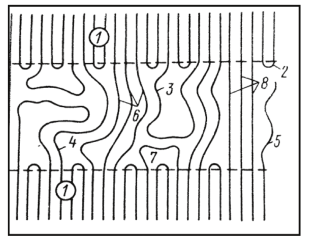
\includegraphics[width=0.6\textwidth]{figures/kinetic_units_scp}
	\caption{Schematic depiction of the kinetic units associated with relaxation transitions in lamellar PE. 1) between the crystalline cores of the lamellas; 2) regular folds with suppressed mobility; 3) irregular loops; 4) folded tie-chains; 5) free ends of macromolecules coming out of lamellas; 6) slightly curved tie-chains; 7) folds the mobility of which is significantly limited by crystallites; 8) fully straightened tie-chains, the ends of which are fixed by neighbouring lamellas. Taken from \cite{arzhakovRelaxationPhysicalMechanical2019}.}
\label{fig:kinetic_units_relax_scp}
\end{figure}

Bowden and Young \citep{bowdenDeformationMechanismsCrystalline1974} provide an early description of the deformation mechanisms in a semi-crystalline polymer not associated with relaxation transitions.
These may include structural changes and lead to permanent deformation.
Drozdov et al. \citep{drozdovViscoelasticityViscoplasticityCreep2009} provide a fairly comprehensive list of such microstructural changes.
In the amorphous phase, orientation of macromolecules along the direction of maximum stress can be observed, as can changes in the concentration of entanglements between chains (junctions in the polymer network), and the formation and growth of micro-voids.
In the crystalline phase, there can be formation and motion of dislocations in the crystallites, rotation and twist of lamellae in spherulites, fine (homogeneous shear of crystal blocks) and coarse (heterogeneous inter-lamellar sliding) slip of lamellar blocks and their fragmentation, micro-necking of lamellae, rotation of lamellar stacks, or rearrangement of the spherulitic structure into a fibrilar structure, among others.
At the interface between the amorphous and crystalline phases, phenomena such as chain slip through the crystals, sliding of tie chains and detachment of chain folds and loops from lamellar block surfaces, diffusion of micro-voids from the amorphous into the crystalline phase, and creation and annihilation of dislocations at lamellae surfaces can all be observed.

Based on several works, e.g., \cite{petersonThermalInitiationScrew1966} and \cite{linRateMechanismPlasticity1994}, Argon \citep{argonPhysicsDeformationFracture2013a} identifies three different interlamellar slip deformation mechanisms in semi-crystalline polymer crystallites: nucleation of a monolithic screw dislocation from the thin edge of the lamella into (100) plane; nucleation of a screw dislocation half loop from the narrow edge; and nucleation of an edge-dislocation half loop from the large flat surface of the wide face of a lamella.

Relevant to the behavior of the amorphous phase, Boyce et al. \citep{boyceLargeInelasticDeformation1988} mention that for glassy polymers, flow is only observed after the segments of the polymer molecules rotate sufficiently to allow it.
It follows the molecular alignment of the polymer chains, resulting in entropy change and increased resistance to the loading.

The nature of the deformation associated with each of these mechanisms is of interest, i.e. whether it is elastic or plastic, recoverable or irrecoverable.
After all, if they lead to flow, it may appear at first glance that the corresponding deformation is always permanent.
Consider this simplified picture: the mechanisms are parallel combinations of dashpots and springs in series, as described in \cite{kellerIdentificationStructuralProcesses1971}.
The differences in the viscosity and stiffness of the springs in this model allow for both permanent deformation and recovery \citep{fotheringhamRoleRecoveryForces1978}.
If some of the mechanisms remained elastic, i.e., the viscosity of the corresponding dashpot is very large, they could even allow for complete recovery.
Physically, it means that the kinetic units responsible for a given flow mechanism may be components of a composite overall structural element whose behavior remains elastic.
Even intralamellar slip in the crystalline part of a semi-crystalline polymer can show some recovery due to the polymer crystallite structure, e.g., when the slip planes cut across fold planes \citep{kellerIdentificationStructuralProcesses1971}.
The deformation split into recoverable/irrecoverable, elastic/plastic is discussed based on mechanical experiments in Section~\ref{sec:reversible_and_irreversible_deformation}.

Regarding the modeling of the deformation behavior connected to each of these phenomena, some of them accept numerically feasible descriptions, e.g., the plastic flow rule corresponding to the nucleation of dislocation in the crystalline part of the polymer or the strain hardening due to the molecular alignment of the amorphous part of the polymer.
However, there are some hurdles to practical application of these models.
Since semi-crystalline polymers are heterogeneous, the descriptions for the deformation mechanisms may not be directly applicable to the bulk material.
Also the structure of the material changes with deformation and hence the relative importance of each mechanism in the overall deformation behavior.
More details on some of these models are supplied in Chapter~\ref{ch:modeling_semi_crystalline_polymer}.

To better understand how the micro and mesostructure evolve with mechanical loading, consider the split of the stress-strain curve proposed by Strobl and coworkers \citep{hissNetworkStretchingSlip1999, hobeikaTemperatureStrainRate2000, hongModelTreatingTensile2004, hongModelTreatmentTensile2004, naViscousForceDominatedTensileDeformation2006}.
It is based on free shrinkage and step-cycle tests, as well as x-ray scattering experiments on deformed samples.
The results were obtained for PE's with different degrees of crystallinity and molecular weight above the glass transition temperature.

At small strains, below a true strain of approximately \num{0.025}, deformation manifests itself mainly through the soft amorphous layers \citep{patlazhanStructuralMechanicsSemicrystalline2012}.
In fact, according to Nikolov and co-workers  \citep{nikolovMicroMacroConstitutive2000, nikolovMultiscaleConstitutiveModeling2002}, experiments show that interlamellar shear is the dominant deformation mode at small strains for PE.

The onset of local flow processes at the end of the Hookean range through isolated slip processes begins at around a true strain of \num{0.025} \citep{hissNetworkStretchingSlip1999}.
Taking into account that local stresses in two-phase heterogeneous solids may strongly exceed the imposed stress, plastic flow of crystal lamellae may appear locally at fairly low strains \citep{patlazhanStructuralMechanicsSemicrystalline2012}.

A collective onset of sliding processes of the crystal blocks composing the crystal lamellae, which determines the yield point (point B in Figure~\ref{fig:stress_strain_curve_strobl}), at around a true strain of 0.1.

The beginning of a disintegration of the crystal blocks which is followed by fibril formation (point C in Figure~\ref{fig:stress_strain_curve_strobl}) at around a strain of 0.6.
Solid-state deformation of a semi-crystalline polymer normally results in the destruction of the crystallites belonging to the original morphology, followed by reordering to form new crystallites.
Newly formed crystallites are themselves subject to disruption at higher orientation levels, being replaced by a fibrillar morphology  \citep{peacockHandbookPolyethyleneStructures2014}.
According to G'Sell \citep{gsellEvolutionMicrostructureSemicrystalline1994}, it is conceivable that the crystallites begin to undergo fragmentation and unfolding at strains between 0.5 and 1.0.
Chain disentanglement (point D in Figure~\ref{fig:stress_strain_curve_strobl}) happens at around a true strain of 1.

\begin{figure}[htbp]
	\centering
	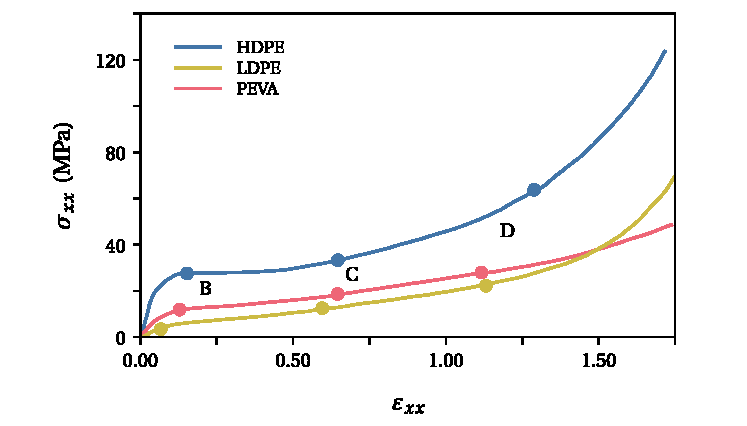
\includegraphics[width=\textwidth]{figures/stress_strain_curve_strobl}
	\caption{Locations of the transition points B-D along the stress-strain curve for HDPE, LDPE and PEVA. Adapted from \cite{hissNetworkStretchingSlip1999}.}
\label{fig:stress_strain_curve_strobl}
\end{figure}

\section{Mechanical response of semi-crystalline polymers}

The thermomechanical response of semi-crystalline polymers is reviewed in this section with the explicit goal of setting targets for constitutive modeling (see Chapter~\ref{ch:modeling_semi_crystalline_polymer} and \ref{ch:numerical_results}).
There are several factors affecting the mechanical response of semi-crystalline polymers.
Extrinsic factors, such as temperature, strain rate, hydrostatic pressure, chemical nature of the environment (the presence of water, oxygen, organic solvents, etc.) are key to describe the behavior of a polymer.
Other relevant elements in the characterization of semi-crystalline polymers are intrinsic.
Of crucial importance are the degree of crystallinity, the lamellar thickness, the mesoscopic structure, molecular weight, physical entanglement and cross-linking, as well as polymer aging \citep{ayoubEffectsCrystalContent2011, serbanTensilePropertiesSemicrystalline2013, callister2014materials, cundiffModelingViscoplasticBehavior2022}.

There are numerous experimental procedures that provide information about a material's mechanical response.
Constant strain rate tests, mostly in the form of uniaxial loading, whether tensile or compressive, but also simple shear and torsion, are among the most relevant for the characterization of semi-crystalline polymers.
Stress relaxation and creep experiments, as well as dynamic mechanical analysis (DMA), are also important tests that highlight the material's time-dependent response.
The polymer's behavior upon unloading must also be considered, using step-cycle and free-shrinkage tests.
The information gathered from these last two experiments will aid in an appropriate discussion of the permanent deformation in semi-crystalline polymers, which is not as easily defined as in most metals at room temperature.
The impact of the previously mentioned factors, such as temperature, strain rate, and hydrostatic pressure, on the mechanical response of the polymer in each type of experiment is thoroughly discussed in next paragraphs.

\subsection{Constant strain rate loading}

The mechanical response of a semi-crystalline polymer in a constant strain-rate experiment is determined by several factors, as discussed above; however, in the conditions typical for most applications, they exhibit the behavior of a plastic polymer, that is, a polymer with some structural rigidity under load suitable for general-purpose applications.
To be considered a plastic polymer, linear and branched polymers must be used below their glass transition temperature, $T_g$, which is supposed to be in the range from \SI{100}{\celsius} to \SI{400}{\celsius} and much higher than their service temperature, $T_\mathrm{ser}$, if amorphous, or below their melting temperature if semi-crystalline \citep{callister2014materials, arzhakovRelaxationPhysicalMechanical2019}.

The stress-strain curves of plastic polymers consistently show a few basic features (see Figure~\ref{fig:response_plastic_polymer}).
The material exhibits a relatively stiff initial response, followed by yielding.
It must be stressed, however, that in most polymers the development of permanent plastic strain is a continuous function of the applied strain, showing no discontinuity at the the nominal stress drop or extrapolated yield point \citep{wardReviewYieldBehaviour1971} (see Remark~\ref{rmrk:yield_polymer}).
After this transient behavior, it follows a steady-state where the stress stabilizes, after which strain hardening begins, intensifying dramatically at large strains \citep{hissNetworkStretchingSlip1999,callister2014materials,makradiTwophaseSelfconsistentModel2005}.
\begin{figure}[hbp]
	\centering
	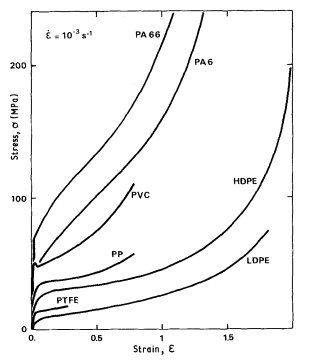
\includegraphics[width=0.9\textwidth]{figures/response_plastic_polymer}
	\caption{Stress-strain curves for different plastic polymers, including both glassy (PVC) and semi-crystaline (LDPE, HDPE, PTFE, PP, PA 6, PA 66) polymers in a constant strain rate uniaxial traction experiment. Adapted from \cite{gsellYieldTransientEffects1981}.}
\label{fig:response_plastic_polymer}
\end{figure}

\begin{remark}[Definition of yield in polymers]
	YYielding is commonly defined as the beginning of plastic flow, for example, when modeling  metals far from their melting temperature, coincides.
	It happens when a critical stress, the yield stress, is reached.

	Polymers, on the other hand, present a more complex situation.
	This is because for many polymers, there may be flow, i.e., "yielding", at any stress level.
	In fact, the initiation of plastic strain is mainly controlled by kinetic processes and appears to play no part in determining the yield point of the material \citep{fotheringhamRoleRecoveryForces1978}, commonly defined in one of three ways: \citep{wardReviewYieldBehaviour1971}
	\begin{itemize}
		\item the stress at the maximum observed load;
		\item the stress corresponding to the point of intersection of two tangent lines on the stress-strain curve;
		\item the stress obtained when offsetting the linear portion of the response by a pre-defined strain amount.
	\end{itemize}
	See a Figure~\ref{fig:yield_criteria} for the corresponding graphical depictions.
	\begin{center}
			\centering
								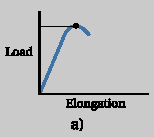
\includegraphics[width=0.3\textwidth]{figures/yield_criterion_a}
				\hfill
							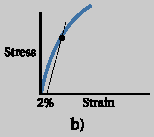
\includegraphics[width=0.3\textwidth]{figures/yield_criterion_b}
			\hfill
								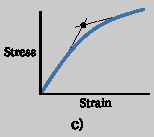
\includegraphics[width=0.3\textwidth]{figures/yield_criterion_c}
		\captionof{figure}{Yield criteria for polymers.}
		\label{fig:yield_criteria}
	\end{center}
\label{rmrk:yield_polymer}
\end{remark}

\paragraph{Pre-yield behavior}
Regarding the response of a semi-crystalline polymer pre-yield, an increase in temperature will lead to a more compliant response and a lower yield strength, as shown, for example, in the results reported in \cite{brownInfluenceMolecularConformation2007} and \cite{hobeikaTemperatureStrainRate2000} for PE's.
In fact, temperature is possibly the single most influential parameter dictating a polymer's mechanical response.
Some polymers may exhibit brittle fracture to necking or even homogeneous rupture during an uniaxial traction test depending on the temperature \citep{wardIntroductionMechanicalProperties2004}.
Moreover, whether the polymer is below or above its glass transition temperature results in markedly different behaviors in the case of amorphous polymers (see Figure~\ref{fig:scheme_effect_temperature} adapted from \cite{vanloockDeformationFailureMaps2018}).
An amorphous polymer in its glassy state behaves as plastic polymer, whereas in its rubbery state it has a much more compliant response, coinciding with very large deformations and a lack of a clear yield point.
On the other hand, even if a semi-crystalline polymer is above its glass transition temperature, the presence of a crystalline phase causes the polymer's response to be qualitatively similar to that of a plastic polymer, although less stiff than it would be at a lower temperature.
See Figure~\ref{fig:response_plastic_polymer} keeping in mind that the glass transition temperature for HDPE is \SI{-90}{\celsius}  \citep{callister2014materials} and the experiment was performed at \SI{22}{\celsius}.
\begin{figure}[hbtp]
	\centering
	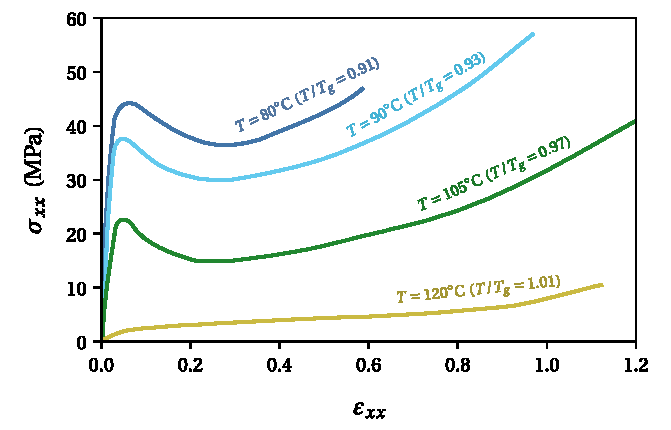
\includegraphics[width=0.9\textwidth]{figures/scheme_effect_temperature}
	\caption{Stress-strain response for poly(methyl methacrylate), an amorhpous polymer, at temperatures very close to its glass transition temperature. Adapted from \cite{vanloockDeformationFailureMaps2018}.}
\label{fig:scheme_effect_temperature}
\end{figure}

The strain rate and the hydrostatic pressure, have the opposite effect, such that their increase will lead to a stiffer response and higher yield stresses, as gathered from the results in \cite{popelarViscoelasticMaterialCharacterization1990} (uniaxial traction) and \cite{trussEffectHydrostaticPressure1981} (torsion).
More specifically regarding the effect of the strain rate on the stress response, Walley and Field \citep{walleyStrainRateSensitivity1994} present experimental results for uniaxial compressive tests on a wide selection of polymers, including semi-crystalline polymers.
The HDPE samples display a linear relationship between the stress at different strain levels and the logarithm of the strain rate, while the PTFE's response shows a non-monotic relationship between the same quantities, which is however broadly increasing.
A linear relationhip between the maximum stress and the logarithm of the strain rate is found for PEEK, until a critical strain rate is reached, followed by a decrease in the stress response.

An increase in bulk crystallinity will lead to a stiffer response and increased strength as evident in the results of Ayoub et al. \citep{ayoubEffectsCrystalContent2011} and Bedoui et al. \citep{bedouiMicromechanicalModelingIsotropic2006} for polyethylenes with degrees of crystallinity by weight at room temperature ranging from 15 to 72\% (see Figure~\ref{fig:deg_cryst_stiff}).
However, the relationship between stiffness and crystallinity appears to be nonlinear.
\begin{figure}
	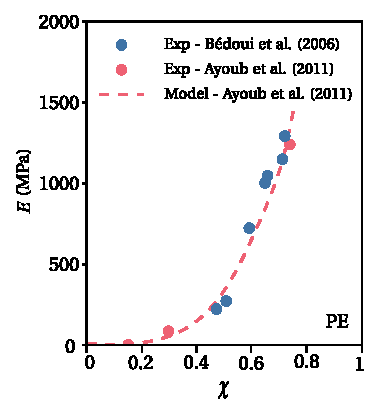
\includegraphics[width=0.6\textwidth]{figures/deg_cryst_stiff}
  \caption{Young modulus of polyethylene as a function of the degree of crystallinity. Results taken from \cite{bedouiMicromechanicalModelingIsotropic2006} and \cite{ayoubModellingLargeDeformation2010}.}
\label{fig:deg_cryst_stiff}
\end{figure}
That said, Schrauwen et al. \citep{schrauwenIntrinsicDeformationBehavior2004} tests in uniaxial compression samples of both PET and PE containing more similar degrees of crystallinity among the samples, 0, 21.7, and 29.7\% and 68.4, 72.3, and 76.6\%, respectively, and no differences in the stiffness are visible in the results.
Clear increases, in the yield strength are, however, noticeable.
The results of Kurtz et al. \citep{kurtzThermomechanicalBehaviorVirgin2002} on UHWPE also support a positive correlation between the degreee of crystallinity and the stiffness as well as the yield strength.
The same authors \citep{kurtzMiniatureSpecimenMechanical1999, kurtzThermomechanicalBehaviorVirgin2002} also explore the effect of cross-linking due radiation combined with changes in crystallinity due to thermal treatments.
A decrease in the elastic modulus and the yield stress with the irradiation dose and the temperature of the thermal treatment is reported.

Schrauwen et al. \citep{schrauwenIntrinsicDeformationBehavior2004} further report that the yield stress is proportional to the lamellar thickness.
However, Argon \citep{argonPhysicsDeformationFracture2013a} mentions, based on results for PE, that this linear dependence is only observed for lamellae of conventional thickness in the range of \SIrange{10}{15}{\nano\meter}.
This dependence eventually breaks down with the yield strength remaining constant for thicknesses from \SIrange{20}{170}{\nano\meter}.
Also, for some polymers, an increase in molecular weigth leads to an increase in the their tensile strength.
This behavior is explained by an increase in chain entanglements with rising molecular weight \citep{callister2014materials}.

Regarding the effect of the mesostructure on the response of a semi-crystalline polymer, when comparing of the stress-strain curves of isotropic and oriented PE, the latter resists deformation more vigorously in the results concerning uniaxial traction presented in \cite{naViscousForceDominatedTensileDeformation2006}.

Finally, the critical strains at which the Hookean range ends or yield is observed are independent of the temperature and strain rate in the ranges considered by Hobeika et al. \citep{hobeikaTemperatureStrainRate2000}, i.e., \SIrange{23}{100}{\celsius} and \SIrange{10e-4}{10e-2}{\per\second}, in PE and PEVA.
In addition, both bulk crystallinity and molecular weight appear to have no impact in the location of these transition points.

\paragraph{Post-yield}
There may be some intrinsic strain softening after yielding, i.e., a decrease in stress with strain.
The results in \cite{schrauwenIntrinsicDeformationBehavior2004} show that after yield is reached, there is a sharp decrease in stress for completely amorphous PET above its glass transition temperature.
The drop becomes broader and less pronounced as crystallinity increases to values of 21.7 and 29.1\%.
The same authors present PE results that show no strain softening for a degree of crystallinity of 76.6\%.
Minor strain softening is visible at lower crystallinity values for the same polymer.
PP softens mildly as well, despite having a crystallinity of around 70\% in the samples studied.
These results were obtained under uniaxial compression, however, no softening is visible after yield in the results of Truss et al. \cite{trussEffectHydrostaticPressure1981} obtained for PE in torsion.
G'sell et al. \citep{gsellApplicationPlaneSimple1983} present results of pure shear experiments in which HDPE exhibit mild strain softening at \SI{23}{\celsius} while PP and PA66 show none.

The presence of strain softening can however change with the strain.
G'sell and Jonas \citep{gsellYieldTransientEffects1981} present the results of an experiment where the strain rate alternates between \SI{1e-3}{\per\second} and \SI{1e2}{\per \second}.
This makes possible the observation of stress transients at different strain levels, when the strain rate switches between the predetermined strain rates.
An unusual behavior is detected in semi-crystalline polymers below the glass transition temperature, such that for lower strains a "normal" transient, i,e,. corresponding to no strain softening, is observed, while at higher strains an "inverse" transient, i.e., coinciding with strain softening, is detected.
The latter type of transient is observable in glassy polymers when the same experiment is performed at any strain level.
The results of Nanzai \citep{nanzaiTransitionMechanismElastic1990} for poly(methyl methacrylate) (PMMA) support this claim regarding the transient behavior of glassy polymers.
According to G'sell and Jonas \citep{gsellDeterminationPlasticBehaviour1979}, an "inverse" transient happens when there are different conditions necessary for the initiation and the propagation of yielding.
Frost and Ashby \citep{frostDeformationmechanismMapsPlasticity1982} mention that such transients are observed in "hard" materials, where dislocations are not readly available, such as lithium floride crystals \citep{gilmanDislocationSourcesCrystals1959, johnstonYieldPointsDelay1962} or diamond \citep{alexanderDislocationsPlasticFlow1969}.

Despite the existence of intrinsic strain softening, its experimental observation is made difficult by two different phenomena: thermal softening and plastic instabilities.
The results presented thus far were obtained at strain rates slow enough to allow for isothermic evolution.
However, as the strain rate increases, a phenomenon known as temperature softening occurs, causing a similar decrease in stress with strain due to an increase in temperature.
This is rise in temperature is a result of the difficulty in offloading the heat generated by the plastic work in such a short period of time, making the process adiabatic.
According to Furmanski et al. \citep{furmanskiTimeTemperatureEquivalence2013}, this effect should be considered at strain rates greater than \SI{0.01}{s^{-1}} and strains greater than 15\%.
Cundiff et al. \citep{cundiffModelingViscoplasticBehavior2022}, for example, reports uniaxial compressive tests for PA 6 where temperature induced strain softening may be observed.

Plastic instabilities, i.e., the growth of a locally thinned region in a material upon application of stresses, must also be considered when the intrinsic response of the material is sought.
They are a function of the geometry and loading conditions of the loaded body, in addition to its intrinsic constitutive behavior \citep{wardIntroductionMechanicalProperties2004}.
While uniaxial compressive loading, in general, doesn't lead to heterogeneous deformation, this is not the case for uniaxial traction experiments, which often, but not always, lead to necking (see the comparison between isotropic and oriented PE in \cite{naViscousForceDominatedTensileDeformation2006}), or simple shear experiments, which may lead to shear banding \citep{gsellApplicationPlaneSimple1983}.
There are however experimental methods which allow for the use of uniaxial traction tests in the determination of intrisic material behavior.
The video-controlled technique in \citep{gsellVideocontrolledTensileTesting1992} is one example, as is the SEÉ method \citep{lauroSEEMethodDetermination2010, balieuDamageHighStrain2015} which uses the full-field data from digitial correlation measurements of heterogeneous displacement fields.

For a material whose stress response depends only on the strain, a maximum in the nominal stress implies the formation of a neck \citep{wardIntroductionMechanicalProperties2004}.
There are also other equivalent criteria, such as Considère's criterion for necking.
Polymers, however, exhibit a strain rate dependence and thus, because necking is associated with a local increase in strain rate, a strong such dependence, can inhibit necking even when the nominal stress reaches a maximum.
For these materials, the existence of a maximum in the nominal stress is only a necessary condition \citep{wardIntroductionMechanicalProperties2004}.
In fact, according to Brooks et al. \citep{brooksModelingDoubleYield1995}, a double yield phenomenon is observed in polyethylenes ranging from LDPE to HDPE.
Lucas et al. \cite{lucasDoubleYieldTensile1995} report similar results for linear polyethylenes and well-characterized ethylene copolymers of narrow molecular weight and composition distributions.
Hao et al. \citep{haoRatedependentConstitutiveModel2022} mention that this phenomenon has also been observed on polyamide (PA), polytrimethyleneterephthalate (PTT) and polybutyleneterephthalate (PBT).
The force maximum observed at the first yield point under certain conditions is therefore to be associated with a homogeneous strain-softening process within the materials and not with the development of the neck (i.e., a geometrical instability) which occurs at the second yield point (see Figure~\ref{fig:double_yield}).
These experimental results make clear that such complex yielding processes are not always observed, being more likely to occur with low crystallinity ratios and low strain rates \citep{zengConstitutiveModelSemicrystalline2010}.
\begin{figure}[htbp]
	\centering
	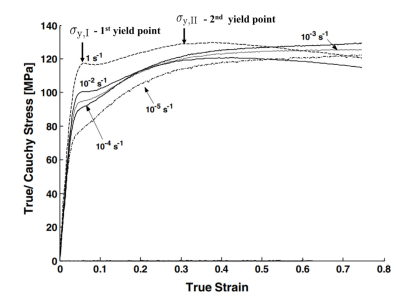
\includegraphics[width=0.7\textwidth]{figures/double_yield}
	\caption{Stress-strain curve for polyethylenes exhibiting double yield. Adapted from \cite{haoRatedependentConstitutiveModel2022}.}
\label{fig:double_yield}
\end{figure}

\cite{yeKinematicStudyNecking2015} reports that for HDPE even with measurements made on a relatively small strain rate range (smaller than 1 decade), the necking phenomenon depends on the strain rate.
In particular, they found that, around the yield point, the strain localization is more pronounced with higher strain rates.

After necking occurs—usually at the maximum load, but not always, as in the case of double yield—the material resists by reorienting the polymer chains, so that the deformation is not limited to the necking zone, as in ductile materials \citep{callister2014materials}.
As the specimen thins from the initial cross-section to the drawn cross-section, the shoulders of the neck travel along it, in what is called cold drawing (see Figure~\ref{fig:natural_draw_ratio}).
The existence of a finite or natural draw ratio, i.e., a strain deformation corresponding to the stable propagation of the neck, is an important aspect of polymer deformation because a stabilized neck is not always formed \citep{wardIntroductionMechanicalProperties2004}.
The neck's stable propagation occurs when the neck area has hardened sufficiently, allowing other sections of the specimen to meet the necking criteria.
If this is the case, Considéré's criterion for necking can be used to determine it.
\begin{figure}[hbtp]
	\centering
	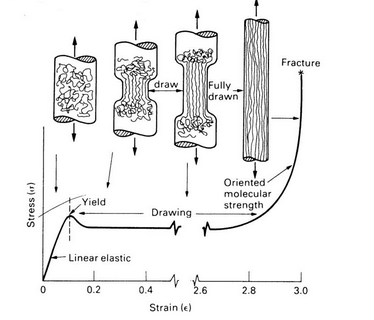
\includegraphics[width=0.6\textwidth]{figures/natural_draw_ratio}
	\caption{Schematic depiction of cold drawing.}
\label{fig:natural_draw_ratio}
\end{figure}

Another important aspect regarding the plasticity of semi-crystalline polymers is that, in contrast to metals, permanent volumetric strains can be detected in addition to elasticity-related volumetric strains.
These effects found both in tension and compression cannot be explained by Hooke's elasticity and correspond to an irreversible contraction or dilation of the material \citep{cangemiTwoPhaseModelMechanical2001,polanco-loriaConstitutiveModelThermoplastics2010}.

Cangemi and Meimon \citep{cangemiTwoPhaseModelMechanical2001} report the existence of plastic dilation in compression for semi-crystalline polymers.
In contrast, for glassy polymers show a very weak contraction.
According to the same authors' results for PA11, the effect of plasticity on volumetric strain is felt when a strain of \num{0.03} is reached.
Until then, the material contracts, after which a significant volume increase is observed.
An increase in confining pressure was also investigated, and the authors discovered that it resulted in a qualitatively similar evolution of the volumetric strain, though it was more pronounced in magnitude, before attaining approximately the same value after a strain of \num{0.16} is reached.
Tensile tests were also performed by the authors, during which the volume strain increases globally, due to the elastic response of the material.
As the material approaches the plastic domain, the total volume strain reduces slightly and then increases again at the end of the test.
Qualitatively identical results were obtained by other authors for PA11 \citep{marchalInfluenceCheminChargement1996}.

Damage, or void growth, is one obvious mechanism responsible for these observations.
However, Polanco-Loria et al. \citep{polanco-loriaConstitutiveModelThermoplastics2010} mention that an increase in volume in semi-crystalline polymers may also be associated with crystalline deformation.
This is because in the crystalline phase the molecules are organized in a rather dense manner, thus the specific volume is likely to increase when the crystalline lamellae break up.
In fact, after a compression test in which the specimens showed net plastic expansion for the majority of the test, Kitagawa and Yoneyama \citep{kitagawaPlasticDilatationDue1988} made thin cuttings of semi-crystalline polymer samples (PP, POM, and PE) for observations in a polarized light microscope.
There were no cracks or crazes found.
This point expresses the peculiarity of plastic volume expansion in semi-crystalline polymers, which may be related to the complexity of their microstructures as well as their two phase nature \citep{cangemiTwoPhaseModelMechanical2001}.

\paragraph{Steady state flow}

After the transient described is cleared and before strain hardening starts to become noticeable there is a period of steady state flow, in which the polymer flows at constant stress function of the temperature and the strain rate.
Both Kurtz et al. \citep{kurtzThermomechanicalBehaviorVirgin2002}, for UHWPE, and G'sell and Jonas \citep{gsellDeterminationPlasticBehaviour1979}, for HDPE, found a reduced strain rate dependendence coinciding with a small coefficient fiting a power law relationship between the stress and the strain rate comparable to metals.
The first authors point out, however, based on their results for UHWPE, that the strain rate sensitivity increases significantly with temperature.

\paragraph{Strain hardening}
Semi-crystalline polymers, if ductile enough, will exhibit strain hardening, which can be quite dramatic at higher strains.
Orientation hardening at large deformation due to molecular alignment is the main source of strain hardening \citep{ahziModelingDeformationBehavior2003}.
In addition to molecular alignement, crystal orientation may also contribute to the strain hardening observed in semi-crystalline polymers \citep{abdul-hameedTwophaseHyperelasticviscoplasticConstitutive2014}.

The results presented by G'Sell and Jonas \citep{gsellYieldTransientEffects1981} at constant strain rate clearly show that at \SI{22}{\celsius} and a strain rate of \SI{1e-3}{\per\second} semi-crystalline polymers such as HDPE, LDPE, PA6 and PA66 show marked strain hardening.
Based on the previously mentioned compressive tests, Schrauwen et al. \citep{schrauwenIntrinsicDeformationBehavior2004} conclude that crystallinity and lamellar thickness have no effect on the strain hardening of semi-crystalline polymers, however the melt cooling procedure and subsequent heat treatments do.
This suggests that the mesostructure may have an effect on the polymer's strain hardening behavior.

\paragraph{Failure}
The maximum strain at rupture for semi-crystalline polymers can be very large, as evidenced by the results of G'Sell and co-workers \citep{gsellYieldTransientEffects1981, gsellApplicationPlaneSimple1983}.
HDPE can reach strains of more than 2 in tensile tests and more than 10 in shear tests.
This is significantly greater than what glassy polymers like PVC and PC can achieve.

\paragraph{Experimental results}

Table~\ref{tab:exp_res_cnst_strain_rate} compiles a sample fo the available experimental results in the literature concerning constant strain rate experiments on semi-crystaline polymers.

\begin{landscape}
\begin{table}[!ht]
\caption{Experimental results concerning constant strain rate experiments.}
\label{tab:exp_res_cnst_strain_rate}
		\small
    \centering
		% \sisetup{range-phrase=--, round-mode=places, round-precision=1, table-format = 1.2e1, table-number-alignment =center, table-figures-exponent=1}
    \begin{tabular}{
		l
		S[round-mode=places, round-precision=0, table-format = 1e1]
		c
		c
		c
		l
		p{8em}
		% p{3em}
		}
		\hline
        Author\vphantom{\Big |} & {Strain rate (\si{\per\second})} & Temperature (\si{\celsius}) & Pressure (\si{\mega\pascal})  & Max strain & Loading mode & Material
				% & Obs
				\\ \hline \hline
        \cite{gsellYieldTransientEffects1981}\vphantom{\Big |} & \SIrange{2e-4}{.9e-1}{} & 22 & Ambient & 1.5 - 2 & Uniaxial traction & HDPE
				% & Transient dip and relaxation-reload curves also included.
				\\
        \cite{gsellYieldTransientEffects1981} & 1e-3 & 22 & Ambient & 1.7 & Uniaxial traction & LDPE, HDPE, PA6, PA66, PTFE
				% & Transient dip and relaxation-reload curves also included.
				\\
        \cite{trussEffectHydrostaticPressure1981} & 9.4e-4 & 20 & \SIrange{1e-1}{4e2}{} & 0.16 & Torsion & Rigidex xxx
				% & ~
				\\
        \cite{popelarViscoelasticMaterialCharacterization1990} & \SIrange{1e-5}{1e-1}{} & 23, 77 & Ambient & 0.25 & Uniaxial traction & MDPE, HDPE
				% & Includes unloading
				\\
        \cite{gsellEvolutionMicrostructureSemicrystalline1994} & 5e-4 & 25 & Ambient & 2 & Uniaxial traction & HDPE
				% & Includes also shear
				\\
        \cite{hissNetworkStretchingSlip1999} & \SIrange{1e-4}{1e-2}{} & Room & Ambient & 2 & Uniaxial & HDPE
				% & ~
				\\
        \cite{hissNetworkStretchingSlip1999} & 5e-3 & Room & Ambient & \SIrange{1.75}{2}{} & Uniaxial traction & HDPE, LDPE, PEVA
				% & Step-cycle tests are also presented.
				\\
        \cite{hobeikaTemperatureStrainRate2000} & \SIrange{1e-4}{1e-2}{} & \SIrange{23}{110}{} & Ambient & 1.8 & Uniaxial traction & HDPE, LDPE, PEVA
				% & The strain split is also analysed.
				\\
        \cite{beijerModellingCreepBehaviour2000} & \SIrange{3.16e-7}{1e-1}{} & 43 & Ambient & 0.25 & Uniaxial & HDPE
				% & ~
				\\
        \cite{schrauwenIntrinsicDeformationBehavior2004} & 3e-3 & Room & Ambient & 0.9 & Uniaxial compression & PE
				% & Comparison between samples with different crystallinity and lamellar thickness.
				\\
        \cite{naViscousForceDominatedTensileDeformation2006} & \SIrange{1e-3}{1e-2}{} & Room & Ambient & 1 & Uniaxial & Oriented HDPE
				% & Step-cycle tests are also included.
				\\
        \cite{drozdovFiniteViscoelasticityViscoplasticity2007} & \SIrange{5e-4}{3e-2}{} & Room & Ambient & 0.2 & Uniaxial traction & LDPE
				% & Tensile
				\\
        \cite{drozdovFiniteViscoelasticityViscoplasticity2007} & \SIrange{5e-4}{1e-1}{} & Room & Ambient & 0.2 & Uniaxial compression & LDPE
				% & ~
				\\
        \cite{brownInfluenceMolecularConformation2007} & \SIrange{1e-4}{2.6e3}{} & \SIrange{-75}{100}{} & Ambient & 0.5 & Uniaxial compression & HDPE, PEX, UHWPE
				% & ~
				\\
        \cite{ayoubModellingLargeDeformation2010} & \SIrange{5e-4}{1e-2}{} & Ambient & Ambient & 2.5 & Uniaxial & HDPE
				% & Includes reloading at different prestrains
				\\
        \cite{zengConstitutiveModelSemicrystalline2010} & \SIrange{2.77e-2}{1.11e-1}{} & 90 & Ambient & 1.5 & Uniaxial traction & PE, PA6
				% & Tensile; includes reloading at different prestrains. Biaxial results are also included.
				\\
        \cite{ayoubEffectsCrystalContent2011} & \SIrange{1e-4}{1e-2}{} & Ambient & Ambient & 1.8 & Uniaxial traction & PE copolymers
				% & Each material has different crystallinity (15\% to 72\%)
				\\
        \cite{furmanskiTimeTemperatureEquivalence2013} & \SIrange{1e-3}{1}{} & \SIrange{-80}{20}{} & Ambient & 0.6 & Uniaxial compression & HDPE, UHMWPE
				% & ~
				\\
        \cite{bergstromMechanicsSolidPolymers2015} & \SIrange{2e-3}{1e-2}{} & - & Ambient & 0.5 & Uniaxial traction & PTFE \\
        \cite{bergstromMechanicsSolidPolymers2015} & \SIrange{2e-4}{2e-2}{} & - & Ambient & 0.35 & Uniaxial & HDPE
				% & ~
				\\
        \cite{ariebyAnisotropicMechanicalBehavior2017} & 1e-3 & Ambient & Ambient & 1.6 & Uniaxial traction & HDPE
				% & Volumetric strain included. Anisotropy also studied.
				\\ \hline \hline
    \end{tabular}
\end{table}
\end{landscape}

\subsection{Stress relaxation, creep  and dynamic mechanical analysis experiments}
\label{sec:relax_creep_dma}

The stress relaxation, creep and dynamic mechanical analysis experiments are all pertinent experiments to characterize the time-dependent behavior of a material.
In particular, the semi-crystalline polymers exhibit a time-dependent behavior that sets them apart, for example, from metals at temperatures far below their melting point.
This section will first focus on isothermic measurements, then on isochronal measurements.

The stress relaxation experiment involves applying a constant strain to the material.
Typically for polymeric systems, the resulting stress response, that is, the so-called relaxation modulus, decreases with time.
A sharp drop is however not noticeable in highly semi-crystalline and glassy polymers, which exhibit stress relaxation moduli in the order of gigaPascals, as depicted in Figure~\ref{subfig:relax_modulus_scp}.
Semi-crystalline polymers with a lower crystalline content exhibit a primary viscoelastic transition from a glasslike to a leathery consistency as a decrease in the stiffness from the order of \SIrange{10e9}{10e7}{\pascal}, as shown in Figure~\ref{subfig:relax_modulus_scp}.
These polymer with a degree of crystallinity between ~5 to 10\% are termed by Tobolsky \citep{tobolskyPropertiesStructurePolymers1960} as very slightly crystalline polymers.
This is similar to the behavior of cross-linked amorphous polymers, since individual molecules may thread in and out of crystalline regions which act as multiple cross-links \citep{ferryViscoelasticPropertiesPolymers1980, gsellYieldTransientEffects1981}.
See, for example, the results of Faucher \citep{faucherViscoelasticBehaviorPolyethylene1959} comparing the relaxation behavior of amorphous and crystalline polypropylene.


This change in the material's response with time is commonly referred to as a transition from a glasslike to a rubberlike (or leatherlike, if a stiffer response is observed) behavior.
However, it is a viscoelastic transition, not the transition verified at the glass transition temperature in which the thermodynamic state of the material changes.
The thermodynamical state of the material remains unchanged in this case, with this particular behavior traceable to the manner in which the kinetic units flow.
Their flow can be described as a thermally activated process where the energetic barriers preventing their motion are cleared with the help of random thermal fluctuations.
The kinetic units have to "wait" until a large enough thermal variation puts them over the hump and they begin moving.
Thus, for very short times the response of the material will be stiffer, as the kinetic units do not have enough time to flow.
As time goes on more and more kinetic units will be able to move leading to a softer response.
Hence, in time dependent materials, the ratio of the time it takes for a material to adjust to applied stresses or deformations, the relaxation time, $t_c$, and the characteristic time scale of an experiment (or a computer simulation), $t_p$, probing the response of the material is especially important.
The Deborah number is the dimensionless quantity defined as this ratio, such that flow will happen when \citep{wardIntroductionMechanicalProperties2004, arzhakovRelaxationPhysicalMechanical2019}
\begin{equation}
	\mathrm{De}=\frac{t_c}{t_p}\approx 1\text{, or  }t_c\approx t_p.
\end{equation}

A constant stress is imposed in a creep experiment, for example, by dead-loading \citep{wildingCreepRecoveryUltra1981}, and an increase in strain is expected over time.
This strain response is the so-called creep compliance of the material.
Glassy polymers and highly crystalline polymers exhibit similar behaviors, with very slow increases in creep compliance with time at the longest times of observation, as do low crystallinity polymers and crosslinked polymers, which exhibit a viscoelastic transition via an increase in compliance as time progresses \citep{ferryViscoelasticPropertiesPolymers1980} (see Figure~\ref{subfig:creep_compliance_scp}).
\begin{figure}[hbtp]
	\centering
	\begin{subfigure}[b]{0.45\textwidth}
							\centering
							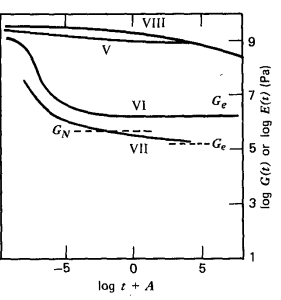
\includegraphics[width=\textwidth]{figures/relax_modulus_scp}
							\caption{}
							\label{subfig:relax_modulus_scp}
			\end{subfigure} \hfill
			\begin{subfigure}[b]{0.45\textwidth}
							\centering
							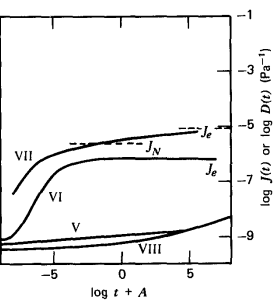
\includegraphics[width=\textwidth]{figures/creep_compliance_scp}
							\caption{}
							\label{subfig:creep_compliance_scp}
			\end{subfigure}
	\caption{\subref{subfig:relax_modulus_scp} Relaxation modulus and \subref{subfig:creep_compliance_scp} creep compliance of a highly and slightly crystalline polymer, as well as a glassy polymer. Adapted from \cite{ferryViscoelasticPropertiesPolymers1980}.}
\label{fig:relax_creep_scp}
\end{figure}

A dynamic mechanical analysis (DMA) employs either a strain or stress driven steady state harmonic oscillation and records the corresponding stress or strain response, respectively.
For a strain driven experiment, the quantities of interest are the storage and loss moduli, defined as the stress response in phase and out phase relative to the strain divided by the strain amplitude, and the loss tangent, which is the tangent of the phase shift between the strain and the stress.
The loss and storage compliances can be defined in a similar way when considering a stress driven experiment.
Their physical interpretation is suggested by their respective names, as they are measures of the energy stored and lost per cycle.
For a perfectly elastic material one would expect no loss, and thus for the stress and the strain to be in phase.
On the other hand, a completely viscous material would exhibit a 90° degree phase shift, dissipating all the energy supplied to the system as heat.
A real material will display an intermediate behavior depending on the frequency.
When $\omega\ t_c \approx 1$, i.e., $\mathrm{De} \approx 1$, for some deformation mechanism with a relaxation time of $t_c$, there will be an increase in the viscous character of the material, hence leading to a drop in  the storage modulus, and maxima in loss modulus and loss tangent (often, not exactly at the same frequency) \citep{ferryViscoelasticPropertiesPolymers1980}.

The storage modulus and compliance are approximately mirror images of the stress relaxation modulus and creep compliance, since a dynamic measurement at frequency $\omega$ is qualitatively equivalent to a transient one at $t=1/\omega$.
The glassy and crystalline polymers have values in the general neighborhood of 0.1 for the tangent loss, and may present several maxima associated with various deformation mechanisms \citep{ferryViscoelasticPropertiesPolymers1980}.
See Figure~\ref{fig:dma_scp} for the loss and storage modulus of highly and lightly crystalline polymers.
\begin{figure}
\centering
\begin{subfigure}[b]{0.45\textwidth}
		\centering
						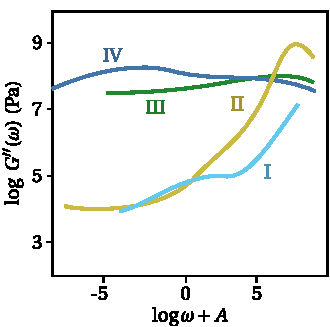
\includegraphics[width=\textwidth]{figures/loss_modulus_scp}
						\caption{}
						\label{subfig:loss_modulus_scp}
		\end{subfigure} \hfill
		\begin{subfigure}[b]{0.45\textwidth}
						\centering
						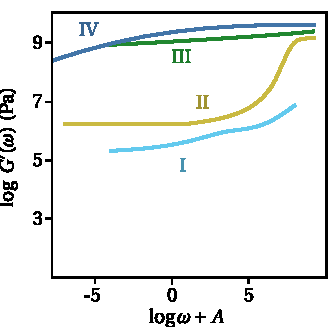
\includegraphics[width=\textwidth]{figures/storage_modulus_scp}
						\caption{}
						\label{subfig:storage_modulus_scp}
		\end{subfigure}
	\caption{Loss \subref{subfig:loss_modulus_scp} and storage \subref{subfig:storage_modulus_scp} modulus of a highly and a lightly crystalline polymer, as well as a glassy polymer. Adapted from \cite{ferryViscoelasticPropertiesPolymers1980}.}
\label{fig:dma_scp}
\end{figure}

Ferry \citep{ferryViscoelasticPropertiesPolymers1980} collects some experimental results illustrating the nonlinear behavior of semi-crystalline polymers.
For a more thorough discussion on what is the expected linear behavior for a time-dependent material see Section~\ref{sec:infinitesimal_thermo_viscoelasticity}.
In a stress relaxation experiment, a linear behavior implies coinciding curves when relaxation modulus divided by the strain is ploted for different strains levels.
However, for tensile stress relaxation of PE single crystal mats, the ratio of stress to strain decreases more rapidly with time at higher extensions, in the range of $\epsilon = \SIrange{0.0003}{0.003}{}$; the degree of nonlinearity increases markedly with decreasing temperature in the range of \SIrange{40}{10}{\celsius}.
Nonlinear creep recovery of polyethylene has also been reported.
It is demonstrated that after a partial stress relaxation at constant strain for various times and strain magnitudes, recovery is much slower at large strains but somewhat faster for shorter durations of the initial straining.
In this system, strains less than 0.01\% appear to be required for a linear behavior.
Nonlinear behavior when subject to sinusoidal deformations with large amplitudes has also been investigated.
Finally, Ben Hadj Hamouda et al. \citep{benhadjhamoudaViscoplasticBehaviourMedium2007} report the existence of two regimes of creep deformation for medium density ethylene-butene copolymer (MDPE).

\begin{remark}[Types of non-linear behavior]
	AAccording, to Malkin \citep{malkinNonlinearityRheologyEssay1995} there are three types of non-linearity in the constitutive response of a material.
	\begin{enumerate}
		\item \textit{geometrical, stationary or weak non-linearity:} characterized by permanent material constants and unchanging relaxation properties. The neo-Hookean behavior of rubbers is one such example;
		\item \textit{physical, kinetic or strong non-linearity:} explained by changes in the inherent structure of a material due to deformation and characterized by changing material constants and relaxation properties with deformation. The hysteresis in repeated deformations of rubbers (Mullins effect) and crystalline polymers;
		\item \textit{phase, thermodynamic or rupture non-linearity:} explained by phase or relaxation transitions induced by deformation and characterized by change in the physical state of the material and radical changes in its relaxation spectrum. The transition of linear polymers from a rubbery to a glassy state is one example.
	\end{enumerate}
\end{remark}

The results previously discussed were obtained at a constant temperature, and are thus isothermal.
Running the tests at different temperatures it is often possible to extend the time/frequency range of the experimental results employing the method of reduced variables, also known as the time-temperature superposition principle, or the thermorheological simple postulate \citep{ferryViscoelasticPropertiesPolymers1980, christensen2013theory}.
It consists in an appropriate horizontal and vertical shift of experimental results obtained at different temperatures to construct a single isothermal master curve.
A physical justification for the applicability of this procedure regarding the horizontal shift can be given in terms of the thermally activated processes that underlie the deformation mechanisms responsible for the relaxation transitions \citep{arzhakovRelaxationPhysicalMechanical2019}
There are several models for the horizontal shift, perhaps the most well known being the site model theory and the Williams, Landel and Ferry (WLF) equation \citep{wardIntroductionMechanicalProperties2004, furmanskiTimeTemperatureEquivalence2013}
A more detailed discussion of the models is given in Section~\ref{sec:viscous_elements}.
A suitable vertical shift can be achieved through the multiplication by $T_0\rho_0/T\rho$, where the subscript 0 denotes a reference state and $T$ and $\rho$ are the temperature and the density, respectively.
Its use is justified due to the entropy-spring nature of the stored elastic energy in the flexible chain theory \citep{ferryViscoelasticPropertiesPolymers1980}.
An application of the time-temperature superposition principle can be found in \cite{popelarViscoelasticMaterialCharacterization1990}, where a master curve is built for a polyethylene employing both horizontal and vertical shifts.

Isochronal results are obtained when the mechanical experiments described in this section are performed at different temperatures and plotted for the same time or frequency.
These are in fact the most common type of available data on semi-crystalline polymers \citep{ferryViscoelasticPropertiesPolymers1980}.
It should be noted that the system's structure changes with temperature, and thus an isothermal plot is, in some respects, more closely and simply related to the distribution of relaxation times than an isochronal plot \citep{hoffmanAnalysisRelaxationsPolychlorotrifluoroethylene2007}.
For example, there are relaxation behaviors that cannot be measured in low crystallinity samples of PCTFE, as it begins to crystallize before the corresponding temperature is reached \citep{hoffmanAnalysisRelaxationsPolychlorotrifluoroethylene2007}.

Focus is given here to results obtained through DMA, although most observations apply to stress relaxation results as well as creep results.
The most important information gathered from these experiments is the temperature of the relaxation transition at a given frequency.
Starting with low crystallinity polymers helps clarify the discussion of relaxation transitions in semi-crystalline polymers.
In fact, for a completely amorphous polymer glass, there will be two important transitions: the alpha and beta transitions.
The alpha transition is tightly connected to the glass transition\footnote{The glass transition is a thermodynamic transition which also implies a structure change in terms of a decrease in the free volume in addition to the cooperative motion of the polymer molecules associated with the alpha viscoelastic transition}, and it is the main viscoelastic transition, while the beta transition is another transition happening at a lower temperature \citep{arzhakovRelaxationPhysicalMechanical2019}.
Which of these happens at higher temperature may change at high enough frequencies \citep{matsuokaThermodynamicTheoryViscoelasticity1996}.
According to Arzhakov \citep{arzhakovRelaxationPhysicalMechanical2019}, the elementary kinetic unit responsible for these transitions is a macromolecule segment, with the beta transition being linked to the quasi-independent, localized displacement of the segments (intramolecule), and the alpha transition, to these quasi-independent modes acquiring a cooperative, coorelated character (intermolecule) \citep{bershteinGeneralMechanismTransition1985, matsuokaThermodynamicTheoryViscoelasticity1996}.
As the extent of crystallinity decreases and amorphous domains large enough to allow configurational rearrangements of longer chain segments appear in semi-crystalline polymers, the motions responsible for these two transitions presumably gradually resemble those seen in the amorphous state in the transition zone of viscoelastic behavior \citep{ferryViscoelasticPropertiesPolymers1980}.

The previously used notation for alpha and beta transitions applies only to amorphous polymers.
In general, semi-crystalline polymer transitions are also classified using the Greek alphabet, but without taking into account the character of the molecular motions corresponding to the transition or the phase in the polymer where it occurs.
The transitions are named alphabetically beginning with alpha in descending order of temperature, resulting in a sometimes confusing literature in which naming is not standardized.
Here, the naming convention will follow the suggestion in \cite{arzhakovRelaxationPhysicalMechanical2019}, using increasing Roman numerals for relaxations verified at increasing temperatures.

Starting at the lowest temperatures, increasing the crystal content of the polymer has little effect on the temperature at which the Relaxation I is verified, resulting in similar loss moduli and loss tangent profiles.
See the results for:
\begin{itemize}
	\item PET ($\beta$ relaxation) by Takayanagi presented in \cite{wardIntroductionMechanicalProperties2004} with degrees of crystallinity of 5, 34 and 50\%, corresponding to \SI{-60}{\celsius} at \SI{138}{\hertz};
	\item for PCTFE ($\gamma$ relaxation) in \cite{mccrumVariationInternalFriction1962} with degrees of crystallinity of 27, 42 and 80\%, corresponding to \SI{-40}{\celsius} at \SI{1}{\hertz};
	\item for PE in \cite{khannaDynamicMechanicalRelaxations1985} with degrees of crystallinity of ~50\% (LDPE) and ~65\% (HDPE), corresponding to \SI{-110}{\celsius} at \SI{1}{\hertz};
	\item for PP in \cite{mccrumStudyInternalFriction1959} with different unspecified degrees of crystallinity, corresponding to \SI{-30}{\celsius} at \SI{1}{\hertz}.
\end{itemize}

However, the temperature at which the next transition, Relaxation II, is verified varies with crystallinity.
For example, for the PE samples studied in \cite{khannaDynamicMechanicalRelaxations1985}, it varied between \SI{-27}{\celsius} and \SI{-10}{\celsius}.
With increasing crystallinity, this relaxation becomes broader and less pronounced.
Relaxation I and II happen in the bulk amorphous phase of the semi-crystalline polymers and the corresponding motions of the kinetic units are the ones responsible by the $\beta$ and $\alpha$ transitions in the completely amorphous polymers.
The disappearance of the relaxations II with the increase in crystallinity is tied to the shrinking of the amorphous domains, and decrease in the number of longer kinetic units responsible for the relaxation.
On the other hand, the relaxations I are connected to motions of smaller kinetic units like the $\beta$ transition in the amorphous polymers, and hence are not affected in the same way by the increase in crystallinity.

The appearance and increase in the size of the crystalline phase will lead to the appearance of a third transition, Relaxation III, at higher temperatures.
This transition is connected to motions on the surface of the crystal lamellae, and the temperature at which is verified vary with their thickness \citep{khannaDynamicMechanicalRelaxations1985, hoffmanAnalysisRelaxationsPolychlorotrifluoroethylene2007}.
Hoffman et al. \citep{hoffmanAnalysisRelaxationsPolychlorotrifluoroethylene2007} present a detailed model of the motions connected to each of the transitions in PCTFE and PE.
Ward and Sweeney \citep{wardIntroductionMechanicalProperties2004} also provide an explanation based on the deformation mechanism available with increasing crystallinity for the "disappearance" of Relaxation II in PE.

According to Arzhakov \citep{arzhakovRelaxationPhysicalMechanical2019}, employing etching techniques that remove the amorphous phase, it can be gathered that the relaxation transitions described so far originate in kinetic units found in the amorphous phase of the polymer.
There is however sometimes a fourth relaxation, connected to the kinetic units in the crystalline phase, and may imply the melting of some of the crystallites.
This transition appears to be visible in the results of Panowicz et al. \citep{panowiczPropertiesPolyethyleneTerephthalate2021} for PET.
It seems, however, not to be noticeable in the other experimental results mentioned so far.
Hoffman et al. \citep{hoffmanAnalysisRelaxationsPolychlorotrifluoroethylene2007} also mention the existence of a cryogenic transition, present in some polymers, such as isotactic propylene (iPP).

As an example of a semi-crystalline polymer that doesn't fit exactly into the classification scheme just provided see the results of McCrum \cite{mccrumStudyInternalFriction1959} for PTFE with crystallinities ranging from 48 to 92\%.
The relaxation observed at the lower temperatures ($\approx$\SI{-100}{\celsius}) disappears with the increase in crystallinity.
In addition, there is a crystalline first order transition ($\approx$\SI{25}{\celsius}), corresponding to the change in crystalline structure of the polymer and a third relaxation at higher temperatures (\SI{125}{\celsius}) that merges with the second when the crystallinity increases.
According to Calleja et al. \citep{callejaWhereGlassTransition2013}, the two relaxations observed at the lowest and highest temperatures correspond to the relaxation of kinetic units in the amorphous phase of the polymer.
The first is the "mobile amorphous fraction," which can relax at low temperatures, and the second is the rigid amorphous fraction, which is composed of macromolecular segments found at the boundaries between crystalline and amorphous domains.
Because of the close proximity of the crystallites, these macromolecular segments have more restricted mobility, and mechanical relaxation occurs at higher temperatures.

%| Author                                                          | Material      | Frequency (Hz) | Temperature (°C) | Crystallinity (%) |
%|:--------------------------------------------------------------- | ------------- |:--------------:| ---------------- | ----------------- |
%| [[mccrumStudyInternalFriction1959\|McCrum (1959)]]              | Polypropylene |       1        |                  |                   |
%| [[mccrumStudyInternalFriction1959\|McCrum (1959)]]              | TFE-HDP copolymers |       1        |                  |                   |
%| [[mccrumVariationInternalFriction1962\|McCrum (1962)]]          | PCTFE         |                |                  |                   |
%| [[wardIntroductionMechanicalProperties2004\|Takayanagi (1963)]] | PET           |      128       |                  |                   |
%| [[khannaDynamicMechanicalRelaxations1985\|Khanna (1985)]]       | Polyethylene  |       1        |                  |                   |


\subsection{Reversible and irreversible deformation}
\label{sec:reversible_and_irreversible_deformation}

The decomposition of the deformation in semi-crystalline polymers into elastic and plastic portions remains to be discussed.
When applied to metals at temperatures far from their melting points, an elastic deformation pertains to the seemingly instantaneous part of the deformation that is recovered upon unloading.
If the metal yields, there will be some plastic deformation that remains after unloading, which is irreversible.
This decomposition is not as clear in the case of time-dependent materials, such as polymers, because there may be deformation that is not immediately recovered upon unloading but is recovered as time passes.
It results in a definition of the irreversible part of the deformation, which is dependent on the observation time, i.e., some deformation may be irreversible during the experiment but potentially reversible if the observation was extended in time.

To clarify which part of the deformation is recoverable and which is irrecoverable the most useful mechanical experiments are the free shrinkage and step cycle tests.
The former consists in straining the sample employing a constant strain rate, and releasing the load as some predefined strain is reached.
The latter also begins as constant strain rate experiment, but after a prescribed time interval has passed the strain rate is reversed until the stress response reaches zero.
Once it does the strain rate is reversed again and enforced for the same time interval as before.
The cycle is repeated until failure or a maximum strain is reached.
During the unloading phases of an applied cyclic deformation process, the response is characterized by nonlinear recovery driven by the release of stored internal energy \citep{bergstromConstitutiveModelingUltrahigh2002}.

Strobl and coworkers \citep{hissNetworkStretchingSlip1999, hobeikaTemperatureStrainRate2000, hongModelTreatingTensile2004, hongModelTreatmentTensile2004, naViscousForceDominatedTensileDeformation2006} performed a very detailed study on polyethylenes which includes the results of both free shrinkage and step cycle experiments.
The decomposition of the constant strain rate stress-strain curve already mentioned above in the text is based on the recoverable and irrecoverable part of the deformation as gathered from these experiments.

Consider the results of step cycle experiments first.
For strains less than 0.025, the polymer is perfectly elastic, and all deformation is immediately recovered.
As the strain exceeds this limit, some deformation will not be recovered immediately.
Reaching 0.1 the proportion of recoverable strain increases relative to the irrecoverable strain.
The former, on the other hand, plateaus once the strain exceeds 0.6 and begins to decrease once the strain reaches 1.
% Unloading behavior studies and permanent plastic deformations in UHMWPE have revealed that classical plasticity theory vastly overpredicts the permanent strains upon unloading \citep{bergstromConstitutiveModelingUltrahigh2002} \colorbox{BurntOrange}{(Maybe add this sentence in the next chapter)}.

So far, only near-immediate recovery has been considered using data from step cycle tests.
To gain a better understanding of the recoverable/irrecoverable deformation decomposition in semi-crystalline polymers, consider the results of free shrinkage experiments.
In the results described in \cite{hissNetworkStretchingSlip1999}, where the deformation was observed for 10 minutes, the amount recovered for the same prestrain is greater than in a step-cycle experiment, as expected.
Similarly, recoverable deformation appears to peak around a strain of 0.6, with low density polyethylene (LDPE) exhibiting a plateau until a strain of 1 is reached.
A distinct plateau is not as visible in high density polyethylene (HDPE) and poly(ethylene-co-vinyl acetate) (PEVA).
However, above strains of 0.6, all experiments show an increase in the amount of irreversible strain.
Bartczak et al. \citep{bartczakEvolutionCrystallineTexture1992} also report that HDPE samples deformed under uniaxial compression showed large amounts of strain recovery upon releasing the load.
They were partly instantaneous and partly over a period of a few hours (<\SI{24}{\hour}).

Finally, Hiss et al. \citep{hissNetworkStretchingSlip1999} report that increasing the temperature in a free shrinkage experiment allows for the recovery of more deformation.
In fact, if the strain does not reach 1 and the temperature used is close to the melting point, almost all of the deformation is recovered.
If the deformation exceeds one, some permanent deformation will remain even after this treatment.
Similarly, Arridge et al. \citep{arridgeSelfhardeningHighlyOriented1977} report that ultra-oriented polyethylene fibers obtained by drawing to approximately 30 times their original length contract on heating to a length near the original.
Furthermore, the same authors investigated the forces that cause this contractile behavior by monitoring the stress in the fiber while keeping its length constant.
Between room temperature and 110°C, the stress decreases as the temperature rises, and this behavior is reversible.
At \SI{120}{\celsius}, there is an irreversible increase in stress, followed by a reversible linear dependence of stress on absolute temperature, indicating elastic entropic forces.
Finally, there are two or three small irreversible stress jumps between \num{124} and \SI{130}{\celsius}, as well as a large irreversible stress increase at around \SI{132}{\celsius}, corresponding to the region of large-scale retraction.
As the fiber relaxes and eventually melts, there is a decay in the stress response.
A fiber allowed to relax in this manner below the melting point differs from a drawn fiber in that it does not exhibit contractile behavior on subsequent heating over a similar temperature range.
Furthermore, despite having a lower tensile modulus after cooling, the modulus and density will rise to values close to their initial counterparts during storage.

% \subsection{Stress dip transient experiment}
%
% Fotheringham and Cherry \citep{fotheringhamRoleRecoveryForces1978} employ a stress dip transient experiment to compute the recovery forces in a semi-crystaline polymer.
% The experiment consists in loading the sample employing a constant strain rate, followed be an unloading which is stoped at a prescribed strain.
% The initial time evolution of the stress is then tracked.
% If it remains constant it signals that the measured stress is equal to the recovery stress.
% Otherwise, if creep, i.e., a stress decrease, or recovery, i.e., a stress increase, are verified it means that the corresponding stress is \colorbox{BurntOrange}{higher} or \colorbox{BurntOrange}{lower} than the recovery stress.
% Multiple attempts with different stoping strains must be attempted to determine the value of the recovery stress.

\section{Thermal analysis techniques}

To fully characterize the thermomechanical behavior of semi-crystalline polymers information about its thermal behavior must be gathered.
This can be obtained from experiments such a dilatometry, differential scanning and laser flash tests \citep{blummCharacterizationPTFEUsing2010}.
The dilatometry experiment consists in tracking the change in volume in a range of temperatures, furnishing the linear thermal expansion of the material.
In principle, the glass transition can be observed in these experiments as a change in the slope of the thermal expansion versus temperature curve.
This is not, however, the case for the results of \cite{blummCharacterizationPTFEUsing2010} concerning PTFE.
What is readily apparent in the results of the same author is the transition in the crystal structure of the polymer, visible a step in the curve.
The evolution of the thermal expansion in the remainder of the temperature range is approximately linear.

The thermal expansion coefficient can also be found through pressure volume temperature (PVT) experiments, as shown in \cite{olaszViscoelasticModelCrossLinked2005} for cross-linked polyethylene (XLPE).
The sample is immersed in mercury and enclosed in a piezometer cell for the experiment.
The cell is contained within a pressure vessel in which hydrostatic pressure can be applied.
After reaching equilibrium at any constant temperature and pressure, the change in specific volume relative to a reference state is recorded.
Measurements were performed from \SI{10}{\mega\pascal} to \SI{200}{\mega\pascal} at \SI{10}{\mega\pascal} increments at temperatures ranging from \SI{25}{\celsius} to \SI{250}{\celsius} at approximately \SI{10}{\celsius} increments, allowing for the determination of the linear expansion coefficient and the bulk modulus as a function of the temperature.

Differential scanning calorimetry is an experimental method of thermal analysis that is widely used to study thermal transitions, i.e., solid-solid transitions as well as solid-liquid and various other transitions and reactions.
The experiment is performed supplying the necessary heat to a test sample as well as a calibrated sample so that a given temperature rate of change is achieved for both.
Excluding the temperatures at which transitions happen, a material with larger heat capacity will require more energy.
If exothermic heat flow is considered the glass transition will appear as a step, cold crystallization as a dip and the melting of crystalline structures as a peak, with the heat capacity of the material being what is measured if these features are removed \citep{lukasDifferentialScanningCalorimetry2009}.

Pope \citep{popeCharacterizationOrientedLowdensity1976} obtains three types of endotherms corresponding to primary melting of the lamellae, to melting of the reorganization products during the scan, and to melting of material crystallized during cooling from the original annealing temperature when studying the melting behavior of samples of oriented low-density polyethylene (LDPE) as a function of annealing temperature and time, subsequent heat treatment, and irradiation dose.
The effect of ionizing radiation on the melting behavior of high-density and low-density
polyethylene is also examined with data obtained by differential scanning calorimetry by Zoepfl et al. \citep{zoepflDifferentialScanningCalorimetry1984}.
The data provided by Blumm et al. \citep{blummCharacterizationPTFEUsing2010} for PTFE makes apparent the solid-solid transition at \SI{23.5}{\celsius} connected to change in crystalline structure of the polymer and the melting of the crystalline phase at \SI{337.3}{\celsius} both as peaks in the results.
In experimental results provided by Panowicz et al. \citep{panowiczPropertiesPolyethyleneTerephthalate2021} for PET in the form of exothermic heat flow the glass transition is apparent as a step around \SI{90}{\celsius} and the melting of crystallites formed during secondary and primary crystallization as dips, the latter much larger than the former.

Finally, \cite{blummCharacterizationPTFEUsing2010} also supplies the thermal diffusivity of PTFE found employing laser flash techniques.
In addition to the change in crystalline of the material already mentioned, the glass temperature is also detectable as a step.
The authors combining the heat capacity, density and thermal diffusivity measurements are able to compute the thermal conductivity of the polymer which is approximately constant across the range of temperatures studied except for the moment when the aforementioned solid solid transition occurs.

\colorbox{BrickRed}{Say something about variation of properties with temperature.}

\chapter{State of the art in thermomechanical semi-crystalline polymer modeling} \label{ch:modeling_semi_crystalline_polymer}

The main goal of this chapter is to report on the semi-crystalline polymer modelling state of the art.
The departure point is infinitesimal thermoviscoelasticity, as it is one of the simplest models available to describe time-dependent materials.
A thorough exposition of its ineadquacies in the description of semi-crystalline polymers is supplied, motivating the introduction of more complex models.

Nonlinear generalizations are considered specifying nonlinear laws for the elastic and viscous elements in rheological models originating from infinitesimal viscoelasticity.
Only properties of a homegenized single phase are taken into account in these models, employed mostly in the description of plastic polymers.
The caveats regarding the generalization to three-dimensions and large deformation are explained, as well as, how to introduce the thermo field into that description.
These are the most commonly available models in the literature and a detailed overview is provided in this chapter.

Following that is a description of models that distinguish between the crystalline and amorphous phases while only considering bulk crystallinity and no additional geometrical information.
Finally, multiscale models with micro and mesostructure considerations are described.

\section{Infinitesimal thermo-viscoelasticity}
\label{sec:infinitesimal_thermo_viscoelasticity}
Given the modeling objectives specified in Chapter~\ref{ch:thermomechanical_behavior_semi_crystalline_polymer}, infinitesimal viscoelasticity presents itself as a satisfactory starting point.
This is because, depending on the model, it can capture strain recovery, creep, stress relaxation, and a transient under monotonic loading, all of which are important features of semi-crystalline polymer mechanical behavior.

Infinitesimal thermo-viscoelasticity, as presented in \cite{christensen2013theory}, fits into the framework of materials with fading memory framework under some restrictions on the material properties (see Section~\ref{sec:thermomechanical_constitutive}).
It is assumed that strains, $\bm \varepsilon$, are small as well as the temperature difference with respect to some reference temperature, $\Delta T=T-T_0$.
Employing the Stone-Weierstrass and Riesz representation theorem, the expression found for the free energy, discarding third order effects, is
\begin{multline}
  \rho\psi(t) = \int_{-\infty}^t \mathbf D(t-\tau):\frac{\partial \bm\varepsilon(\tau)}{\partial \tau}d\tau + \int_{-\infty}^t \beta(t-\tau)\frac{\partial \Delta T(\tau)}{\partial \tau}d\tau\\ + \frac{1}{2}\int_{-\infty}^t\int_{-\infty}^t \frac{\partial \bm\varepsilon(\eta)}{\partial \eta}:\mathbf G(t-\tau, t-\eta):\frac{\partial \bm \varepsilon(\tau)}{\partial \tau}d\tau d\eta + \\
  -\int_{-\infty}^t \int_{-\infty}^t \bm\varphi(t-\tau, t-\eta):\frac{\partial \bm\varepsilon(\tau)}{\partial \tau} \frac{\partial \Delta T(\eta)}{\partial \eta} d \tau d \eta\\
  -\frac{1}{2} \int_{-\infty}^t \int_{-\infty}^t m(t-\tau, t-\eta) \frac{\partial \Delta T(\tau)}{\partial \tau} \frac{\partial \Delta T(\eta)}{\partial \eta} d \tau d \eta,
  \end{multline}
where $\mathbf D$, $\beta$ , $\mathbf G$, $\bm \varphi$ and $m$ are appropriate functions describing  material properties.
In particular, the last three quantities are the counterparts in infinitesimal thermoviscoelasticity to the stiffness tensor, the coefficient of thermal stress and the specific heat at constant deformation, respectively, in infinitesimal thermoelasticity.

The constitutive relations found concerning the stress and the entropy are
\begin{gather}
  \bm \sigma(t) = \int_{-\infty}^t \mathbf G(t-\tau, 0):\frac{\partial\bm\varepsilon}{\partial \tau} d\tau-\int_{-\infty}^t \bm\varphi(0, t-\tau)\frac{\partial \Delta T(\tau)}{\partial \tau},\\
  \rho s(t) = \int_{-\infty}^t \bm\varphi(t-\tau, 0):\frac{\partial \bm \varepsilon}{\partial \tau} + \int_{-\infty}^t m(t-\tau, 0)\frac{\partial \Delta T(\tau)}{\partial \tau}.
\end{gather}

Regarding the dissipation, its magnitude is of second order and as such can be discarded in this infinitesimal theory.
This implies a small perturbation away from thermodynamic equilibrium.

The stress-strain relationship for the isothermal case is given by a convolution integral, coinciding with the description of linear time invariant system (LTI), as
\begin{equation}
\label{eq:stress_constitutive_infinitesimal_viscoelasticity}
	\bm \sigma(t) = \int_0^t \mathbf G(t-\tau):\frac{\partial \bm \varepsilon(\tau)}{\partial \tau}\ d\tau,
\end{equation}
where $\mathbf{G}$ is the relaxation modulus of the material.

Furthermore, in some cases, this description is equivalent to an ordinary differential equation involving stress, strain, and their corresponding time derivatives.
Often, these can be identified with the behavior of linear rheological models, which provide a visual counterpart and help in the interpretation of the model.
These are one-dimensional mechanical models containing diverse arrangements of linear springs and dashpots.
For an in depth discussion on the connection between LTIs and ordinary differential equations see \cite{ciampaLinearDifferentialEquations2019}.

In general, the relaxation modulus can also be written as \citep{malkinRheologyConceptsMethods2017}
\begin{equation}
\label{eq:relax_mod_decomp}
	G(t) = G_\infty + \varphi(t),
\end{equation}
where $G_\infty$ is the equilibrium modulus and $\varphi$ is the relaxtion function.
From its physical meaning, the latter is a decreasing function of time having zero limit at $t\to\infty$.
The functions of such type can always be presented by the following integral
\begin{equation}
  \label{eq:relax_time_spectrum}
	\varphi(t) = \int_0^\infty H(\theta) e^{-t/\theta}\ dT,
\end{equation}
where $\theta$ denotes the relaxation time, and $H$ is a function of the distribution of the relaxation times, the so-called, relaxation time spectrum.

For example, considering the so-called Burgers material, the relaxation modulus, $G$, is given by \citep{malkinRheologyConceptsMethods2017}
\begin{equation}
\label{eq:relaxation_modulus_burgers}
  G(t)=G_{1} e^{-t / \theta_{1}} + G_2 e^{-t/\theta_2},
\end{equation}
where $\theta_i$ is the $i$th relaxation time, so that the constitutive relation in the one-dimensional case is also given by
\begin{equation}
  \sigma + \left(\frac{\eta_1}{G_1} + \frac{\eta_2}{G_2}\right) \dot \sigma + \frac{\eta_1\eta_2}{G_1G_2}\ddot \sigma = (\eta_1 + \eta_2)\dot\varepsilon + \frac{\eta_1\eta_2(G_1 + G_2)}{G_1G_2}\ddot\varepsilon,
\end{equation}
where $\eta_i$ is the viscosity of the $i$th dashpot, $G_i$ is the stiffness of the $i$th spring, and $\dot{\bullet}$ denotes the derivative with respect to time.
Given the definition in Equation~\eqref{eq:relax_time_spectrum}, the relaxation time spectrum for the Burgers material is given by
\begin{equation}
  H(\theta) = G_1 \delta(\theta - \theta_1) + G_2 \delta(\theta - \theta_2),
\end{equation}
where $\delta$ is the $\delta$-Dirac function.
See Figure~\ref{fig:burgers_mat} for the corresponding rheological model.

The ordinary differential equations describing these models can also be transformed into a state space representation, where the description of the systems state is made through state variables.
Also, for Burgers material, an equivalent description can be found as
\begin{align}
\label{eq:state_var_desc_burgers}
	\sigma &= G_1\varepsilon_{e,1} + G_2\varepsilon_{e,2},\\
	\dot \varepsilon_{e,1} &= -\frac{\eta_1}{G_1}\varepsilon_{e,1} + \dot \varepsilon,\\
	\dot \varepsilon_{e,2} &= -\frac{\eta_2}{G_2}\varepsilon_{e,2} + \dot \varepsilon,\\
\end{align}
where $\varepsilon_{e,i}$, $i=1,2$, is the strain in the $i$th spring, as well as, an internal variable of the constitutive model.
Their evolution can be tied to transient effects, such as the ones observed at the beginning of monotonic loading at a constant strain rate in the case of a Burger material (see Figure~\ref{subfig:burgers_cnst_strain_rate}).
Figures~\ref{subfig:burgers_stress_relax} and \ref{subfig:burgers_creep_plus_recov} illustrate the response of the Burgers material to a constant strain and a constant stress followed by release, respectively, illustrating the ability of the model to capture the phenomena of strain recovery, creep and recovery.
\begin{figure}
\centering
\begin{subfigure}[b]{0.30\textwidth}
            \centering
            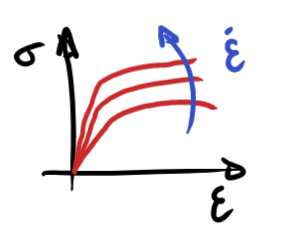
\includegraphics[width=\textwidth]{figures/burgers_cnst_strain_rate}
            \caption{}
            \label{subfig:burgers_cnst_strain_rate}
    \end{subfigure} \hfill
    \begin{subfigure}[b]{0.30\textwidth}
            \centering
            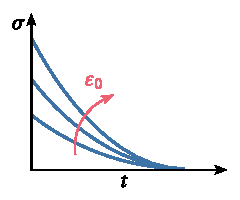
\includegraphics[width=\textwidth]{figures/burgers_stress_relax}
            \caption{}
            \label{subfig:burgers_stress_relax}
    \end{subfigure}
    \hfill
    \begin{subfigure}[b]{0.30\textwidth}
      \centering
      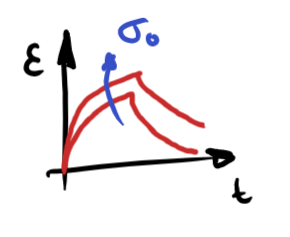
\includegraphics[width=\textwidth]{figures/burgers_creep_plus_recov}
      \caption{}
      \label{subfig:burgers_creep_plus_recov}
    \end{subfigure}
  \caption{Respnse of the Burgers material in \subref{subfig:burgers_cnst_strain_rate} constant strain rate experiment, \subref{subfig:burgers_stress_relax} a stress relaxation experiment and a \subref{subfig:burgers_creep_plus_recov} creep experiment with recovery.}
\label{fig:burgers_mat_res}
\end{figure}

\begin{remark}[Choice of internal variables]
  A state variable is one of the set of variables that are used to describe the mathematical "state" of a dynamical system. Intuitively, the state of a system describes enough about the system to determine its future behaviour in the absence of any external forces affecting the system.
  In general, they can be identified with the rheological elements able to storage energy, i.e., with the springs.
  To see may the strain in the viscous element, may not be an appropriate choice consider, in the case of the Burgers material (see Equation~\eqref{}), a relaxation experiment where the strain is unknown and the external force is the strain rate which is zero.
  Knowing the strain on the springs the the stress can be easily found and from these the evolution of the elastic strain from the flow rule.
  If it was the viscous strains knwon not much could be done.
  \colorbox{BurntOrange}{Include also stuff about structure.}
\end{remark}

\paragraph{Linearity}
It is worth noting that infinitesimal thermoviscoelasticity is linear, in the sense that the response to the sum of two inputs is the sum of the responses to each of the inputs (see Figure~\ref{fig:linearity}).
In the context of viscoelasticity, this principle is called the Boltzmann-Volterra superposition principle \citep{wardIntroductionMechanicalProperties2004}.
Thus in the one-dimensional case, for discrete increases in strain $\Delta \varepsilon_i$ at instants $\tau_i$, $i=1,2,3,\dots$, the stress is given by
\begin{equation}
	\sigma (t) = \Delta \varepsilon_1 G(t - \tau_1) + \Delta \varepsilon_2 G(t - \tau_2) + \Delta \varepsilon_3 G(t - \tau_3) + \cdots
\end{equation}
If the increases in strain considered are rendered infinitesimal, the constitutive law found for the stress is the convolution integral in Equation~\eqref{eq:stress_constitutive_infinitesimal_viscoelasticity}.
This is entimately connected to the fact that the rate equations for the state variables are ordinary differential equations (see Equation~\eqref{eq:state_var_desc_burgers} for the Burgers material) and that as a material property, the relaxation modulus is only a function of time and not of strain, strain rate or stress (see Equation~\eqref{eq:relaxation_modulus_burgers} for the Burgers material).
The consequences of this linear behavior for the response of the material in relevant mechanical experiments are discussed shortly.
\begin{figure}[hbtp]
  \centering
  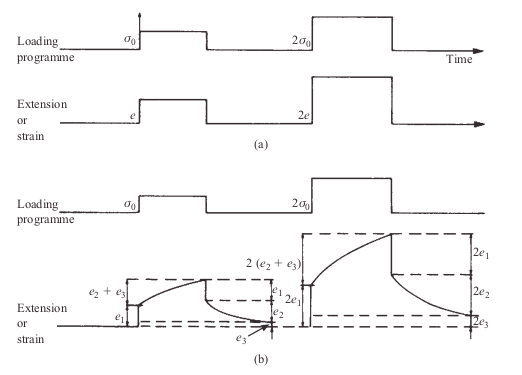
\includegraphics[width=0.6\textwidth]{figures/linearity}
  \caption{Linearity in the deformation of an elastic, a viscous, and a viscoelastic material. Adapted from \cite{wardIntroductionMechanicalProperties2004}.}
\label{fig:linearity}
\end{figure}

\paragraph{Limitations of infinitesimal viscoelasticity}
Infinitesimal viscoelasticity has however some major limitations, first among them the use of infinitesimal strains in the constitutive description of the material.
Semi-crystalline polymers, such as HDPE, can frequently achieve true strains in axial tests that exceed 1.5, far surpassing what could be considered small deformations \citep{gsellYieldTransientEffects1981}.

Furthermore, the Boltzmann superposition principle is frequently violated, and there is energy exchange between the different relaxation modes, implying that the relaxation modulus depends on strain, strain rate, and/or stress.
Semi-crystalline polymers exhibit nonlinear behavior that can be detected in a variety of mechanical experiments.
References to experimental results depicting this behavior can be found in Section~\ref{sec:relax_creep_dma}.
A comparison between a linear response and possible non-linear responses to the most common mechanical experiments is provided in what follows to understand the deficits of infinitesimal viscoelasticity.

Firstly, consider constant strain rate experiments ran at different strain rates.
At some point (see Equation~\eqref{eq:relax_mod_decomp}), a steady state will be reached, meaning $\dot \alpha = 0,$ and the corresponding response in an infinitesimal viscoelastic model is either constant (liquid) or linear (solid) in the strain.
At any rate, for a given strain, the stress varies linearly with the strain rate and is proportional to the relaxation time, corresponding to so-called Newtonian viscosity \citep{matsuokaThermodynamicTheoryViscoelasticity1996} (see Figure~\ref{subfig:constant_strain_rate_expected}).
Neither of these two facts is always observed in practice.
For example, HDPE displays a strong hardening, as shown in the experimental results of, e.g., \cite{gsellYieldTransientEffects1981}, which is not linear in the strain, i.e., its stiffness varies with the strain (see Figure~\eqref{subfig:constant_strain_rate_nonlinear}).
Also, the stress corresponding to the steady state as a function of the strain rate often follows a power law (see e.g.,  \cite{gsellDeterminationPlasticBehaviour1979}) coinciding with so-called non-Newtonian viscosity (see Figure~\ref{fig:constant_strain_rate_expected}).
Besides this, Matsuoka \citep{matsuokaThermodynamicTheoryViscoelasticity1996} emphasizes that for infinitesimal viscoelasticity, the steady state stress grows unbounded with the strain rate according to the model of infinitesimal viscoelasticity, which makes no physical sense.
Also, some semi-crystalline polymers exhibit more or less abrupt changes in flow behavior at a given stress, which is akin to plastic yield in rate-independent plasticity \citep{bergstromMechanicsSolidPolymers2015}.
\begin{figure}
\centering
  \begin{subfigure}[b]{0.45\textwidth}
            \centering
            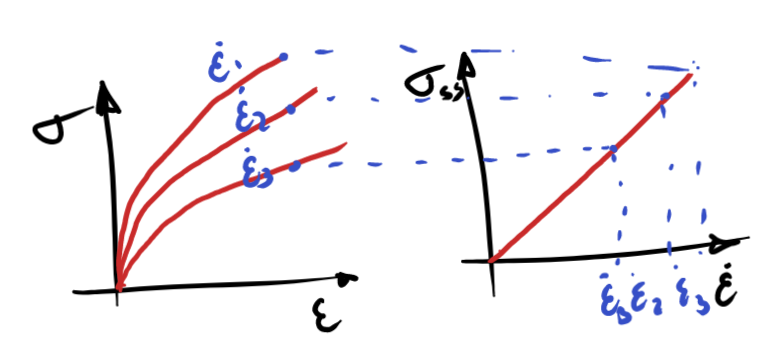
\includegraphics[width=\textwidth]{figures/constant_strain_rate_expected}
            \caption{}
            \label{subfig:constant_strain_rate_expected}
    \end{subfigure} \hfill
    \begin{subfigure}[b]{0.45\textwidth}
            \centering
            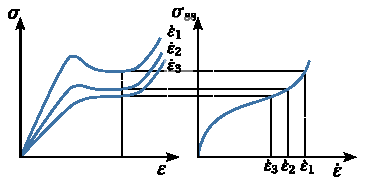
\includegraphics[width=\textwidth]{figures/constant_strain_rate_nonlinear}
            \caption{}
            \label{subfig:constant_strain_rate_nonlinear}
    \end{subfigure}
  \caption{Stress-strain curve and Steady state stress-strain rate curve for a \subref{subfig:constant_strain_rate_expected} an infinitesimal viscoelastic material (linear) and a \subref{subfig:constant_strain_rate_nonlinear} nonlinear material.}
\label{fig:constant_strain_rate_results}
\end{figure}

Another nonlinear feature observed in semi-crystalline polymers is the dependence of the relaxation modulus and creep compliance on the strain and stress, in addition to time.
The expected linear behavior in a stress relaxation experiment is to obtain the same stress response up to a multiplicative constant, which is the initial strain.
Likewise, in a creep experiment the strain response divided by the stress is equal for experiments at different stress levels.
See Figure~\eqref{fig:relax_creep_expected} for a depiction of the expected linear and possible nonlinear behaviors.
The recovery may also display nonlinear features, that is, the strain recovered $\varepsilon_r$ will also depend on the initial strain $\varepsilon_0$ and how long the sample was strained, $t_0$, yielding completly different $\varepsilon/\varepsilon_0$ versus $\log t/t_0$ curves \citep{ferryViscoelasticPropertiesPolymers1980}.
\begin{figure}
  \includegraphics[width=0.9\textwidth]{example-image-a}
  \caption{Expected behavior of a infinitesimal viscoelastic material and nonlinear alternatives in a) stress relaxation experiment, b) in a creep experiment. }
\label{fig:relax_creep_expected}
\end{figure}


\section{Finite linear viscoelasticity}
The infinitesimal viscoelatic model can be derived assuming that the stress depends only on the "magnitude" of the deformation history to the first order (see \cite{colemanFoundationsLinearViscoelasticity1961} or \cite{christensen2013theory}).
This is automatically satisfied if only small strains are considered.
However, Coleman and Noll \citep{colemanFoundationsLinearViscoelasticity1961} point out that finite deformations can also be considered, as long as the motion is slow enough when compared with the material's rate of "forgeting".
The stress strain constitutive relation is still described as a convolution integral (see Equation~\eqref{eq:stress_constitutive_infinitesimal_viscoelasticity}), and may be frequently described by ordinary differential equations, where instead of the infinitesimal strain tensor, a strain measure compatible with finite strains, e.g., the Green-Lagrange strain tensor, can be employed.
This approach to viscoelasticity allows for finite strains, however it is still linear with respect to the strain measure,--not the displacement, since the former are nonlinear functions of the latter--, thus, respecting the Boltzman superposition principle and keeping the relaxation spectrum depending only on time.
As such, this model won't display most of the required nonlinear effects observed in semi-crystalline polymers and described in the previous chapter.
In addition, since the dissipation is a second order effect, the state of the material remains close to thermodynamical equilibrium, so that the dissipation will not contribute as a source in the energy equation (Equation~\eqref{eq:heat_conduction}).

\section{Single integral models}
Another set of approaches that seeks to generalize the results of infinitesimal viscoelasticity is based on the integral constitutive equation for the stress as a function of the strain in Equation~\eqref{eq:stress_constitutive_infinitesimal_viscoelasticity}.
These models include nonlinear phenomena while considereing only small strains \citep{wardIntroductionMechanicalProperties2004}.
For example, the model of Pipkin and Rogers is given by \citep{wardIntroductionMechanicalProperties2004}
\begin{equation}
	\sigma(t) = \int_{-\infty}^t R(t-\tau, \varepsilon(\tau))\frac{\partial \varepsilon}{\partial \tau}\ d\tau,
\end{equation}
where $R$ is a nonlinear stress relaxation modulus depending on both time and strain, incorporating nonlinear effects into the material's infinitesimal viscoelastic constitutive description.

A list of models of this type, including the models of Leaderman, Pipkin and Rogers, Schapery, and Bernstein, Kearsley and Zapas (BKZ) can be found in \cite{wardIntroductionMechanicalProperties2004} and \cite{malkinRheologyConceptsMethods2017}.
According to Ward and Sweeney \citep{wardIntroductionMechanicalProperties2004}, Smart and Williams \citep{smartComparisonSingleintegralNonlinear1972} assessed the three models' performance when applied to tensile stretching of polypropylene and poly(vinyl chloride) fibers, but only up to modest strains (4\%).
At these strains, the BKZ model proved to be of limited interest, while the Pipkin and Rogers model, albeit being simpler than Schapery's theory, yielded a somewhat inferior result.
Moreover, Turner \citep{turnerStrainResponsePlastics1966} concludes about single integral models that viscoelastic behavior in general cannot be discussed simply in terms of a stress-strain-time relationship and a modified superposition integral.

With particular relevance to the modeling of semi-crystalline polymers, Popelar \citep{popelarViscoelasticMaterialCharacterization1990} modeled MDPE and HDPE employing Schapery's nonlinear viscoelasticity with good results.
The experimtal test used for vaidation included constant strain rate uniaxial traction tests with strain rates ranging from \SIrange{10e-5}{10e-1}{\per\second} and temperatures from \SIrange{23}{77}{\celsius} and a maximum strain of 0.25.
Regarding the free energies corresponding to these stress-strain constitutive relationhips, Gurtin and Hrusa \citep{gurtinEnergiesNonlinearViscoelastic1988} present a discussion on the topic.
This class of models will not be discussed further in the text since, due to their formulation in terms of convolution integrals, they are not particularly appropriate for application in computational mechanics.

\section{Descriptions based on rheological models wiht nonlinear elements}

A viscoelastic constitutive model fit for large strains and capable of capturing the required nonlinear behaviors can often be achieved by specifying nonlinear laws for the behavior of the elements in a rheological model.
It is by far the most common approach, and to introduce it, the laws available for viscous elements are presented first, followed by the corresponding laws for elastic elements.
The necessary kinematic decomposition to produce a large strain three-dimensional  is discussed as well as the changes needed for the introduction of the thermal field.
Finally, the most relevant models available in the literature that follow this approach.

% \begin{remark}[Phenomenological vs. First principles]
% 	A phenomenological model rests on fitting parameters and empirical assumptions.
% 	A first principle rests on reasoning from first principles.
% 	What are first principles? It depends on the chosen abstraction level.
% 	We have continuum mechanics, kinetic theory/statistical mechanics, molecular dynamics and quantum mechanics.
% 	Here only continuum mechanics and kinetic theroy are considered.
% 	Give examples? What moves from one to the other? \colorbox{BrickRed}{Complete this!!!!}
% \end{remark}

\subsection{Viscous elements}
\label{sec:viscous_elements}

Plastic flow is a kinetic process, as pointed out by Frost and Ashby \citep{frostDeformationmechanismMapsPlasticity1982}, therefore, the strength of a solid depends on both strain and strain-rate, in addition to the temperature.
This runs counter to the useful concept of a yield strength, below which there is no flow and above which flow is fast.
According to the same authors, this would only be strictly true at absolute zero.
The corresponding theoretical flow stress is often called the mechanical threshold or athermal strength.
Furthermore, flow below that mechanical threshold is due to thermally activated kinetic processes, i.e., their rate depends on the thermal fluctuations of the kinetic units.
For the sake of completeness, it should be mentioned that there are kinetic processes that become relevant when the loading exceeds the mechanical threshold, coinciding with very high strain rates, and which do not necessitate thermal activation to occur \citep{kocks1975thermodynamics}\footnote{In the context of polycrystalline materials, where slip is the main deformation mechanism the former correspond to so-called jerky glide and the latter to continuous glide \citep{kocks1975thermodynamics}.}.
These are beyond the scope of the present work.

To better understand how thermal fluctuations allow for flow, consider that at a given temperature in a solid, the kinetic units perform thermally driven oscillations of random magnitude near an equilibrium position.
If the motion of the kinetic units coincides with their permanence near that equilibrium state the behavior of the solid will be elastic.
On the other hand, flow happens when the energetic barrier $\Delta H$ bounding the equilibrium state and corresponding to a transition state, is cleared.
This is the energy of activation at \SI{0}{\kelvin} when no force is acting on the material \citep{kocks1975thermodynamics}.
Employing the Boltzmann distribution from statistical mechanics to calculate the probability of a thermal fluctuation providing enough energy to overcome the energy barrier, the rate of transition between states is given in the form of the Arrhenius equation, written in this context as
\begin{equation}
	k = A\exp\left(-\frac{\Delta H}{k_BT}\right),
\end{equation}
where $k_B$ is Boltzmann's constant, $A$ is the pre-exponential factor, $\varepsilon_0$ is the height of the energy barrier.
The pre-exponential term can be interpreted as the rate of attempts to move over the transition state \citep{atkins2010atkins}.
According to Kocks et al. \citep{kocks1975thermodynamics}, it is related to one of two extreme frequencies: either the "atomic" frequency, i.e., the frequency of uncorrelated atomic motions, or the kinetic unit ground frequency, correlated with the overcoming of many of obstacles at the same time.
The inverse of the this rate, i.e.,
\begin{equation}
	\theta = \frac{1}{A}\exp\left(\frac{\Delta H}{k_B T}\right),
\end{equation}
is the relaxation time of the process.

To consider the effect of applying a stress to the material, take into account that the work provided by that stress will be discounted from the total energy required to overcome the kinetic unit's obstacle to motion.
The free Gibbs energy, also known as free enthalpy, is that missing portion of energy that must be supplied by a thermal oscillation.
Without factoring in the thermal fluctuations, the motion would occur only if the work supplied by the stress was larger than the energy barrier.
Moreover, if the free energy of the kinetic unit is greater after crossing the barrier, some of the plastic work was not dissipated, some energy remaining latent in the material.
On the other hand, the free enthalpy of the kinetic unit is always lower after crossing the barier; otherwise, there would be no greater probability of crossing in one direction than the other (see Figure~\ref{fig:site_model_theory}).
For more details see \cite{kocks1975thermodynamics}.
\begin{figure}
	\centering
	\includegraphics[width=0.9\textwidth]{example-image-a}
	\caption{Transition of a kinetic unit between two states. a) Free energy. b) Free enthalpy.}
\label{fig:site_model_theory}
\end{figure}

Thus, following the procedure outlined by Eyring \citep{eyringViscosityPlasticityDiffusion1936}, the shearing force acting on the system and its effect on the flow of the kinetic units can be considered.
Its presence will lead to a different rate of jumps in the forward and backward directions, which in energetic terms means lowering the energy of the final state and increasing the energy of the initial state.
Assuming similar activation volumes, and subtracting the rate of kinetic units moving against the shearing force from those moving along with the shearing force, $\tau$, the strain rate obtained is
\begin{equation}
	\label{eq:eyring_model}
	\dot \gamma = \dot\gamma_0 \exp\left(-\frac{\Delta H}{k_BT}\right)\sinh\left(\frac{v\tau}{k_BT}\right),
\end{equation}
where $v$ is the so-called activation volume, and it can be identified with the product of the area swept out by the mobile unit in moving from one local free energy minimum to the next and the resolved component in the direction of the applied stress of the distance moved by the kinetic unit.

According to the same author, for ordinary flow, $v\tau$ is much smaller than $k_B T$, thus, the expression for Newtonian viscous flow is recovered as
\begin{equation}
  \label{eq:newton_fluid_flow_rule_scalar}
	\dot \gamma = \frac{\dot \gamma_0 v}{k_B T}\exp\left(-\frac{\Delta H}{k_BT}\right)\tau=\frac{1}{\eta}\tau,
\end{equation}
where $\eta$ is the viscosity.
On the other hand, for plastic flow, when $\tau$ is large, the flow rule comes out to be
\begin{equation}
\label{eq:flow_rule_thermally_activated}
	\dot\gamma = \dot \gamma_0 \exp\left(-\frac{\Delta H - v \tau}{k_B T}\right)=\dot \gamma_0 \exp\left(-\frac{\Delta G(\tau)}{k_B T}\right),
\end{equation}
which coincides with a negligible rate in the backwards direction.
The contribution of hydrostatic pressure can also be accounted for in this framework in a similar way to the shearing force, i.e.,
\begin{equation}
	\dot\gamma = \dot\gamma_0 \exp\left(-\frac{\Delta H - v \tau + \Omega p}{k_B T}\right),
\end{equation}
where $\Omega$ is the activation volume corresponding to the hydrostatic pressure.
This can be justified in terms of experimental results, where the stress response of polymers shows a pressure dependence, in part due to the low bulk moduli of polymers (~\SI{5}{\giga\pascal}, compared with metals ~\SI{100}{\giga\pascal}) \citep{wardIntroductionMechanicalProperties2004}.
A suitable expression for the effective stress on the kinetic units is found to be a linear combination of shear stress and hydrostatic pressure, similar to the Mohr-Coloumb yield criterion.
From the expressions, it is clear that higher shear stresses lead to higher flow rates, with the hydrostatic pressure having the reverse effect.

According to Fotheringham and Cherry \citep{fotheringhamRoleRecoveryForces1978} it is not clear that the activation volumes in the forward and backward direction are the same.
However, note that when the expression is employed to describe plasticity this is not relevant, as only one activation volume has to be considered.
In fact, more general rate equations for thermal activated flow can be found in \cite{brinkmanMechanicalThermodynamicalTheory1957} or \cite{kocks1975thermodynamics}.

The experimental determination of the parameters in these models are discussed, e.g., in \cite{evansThermallyActivatedDeformation1969}, \cite{conradAthermalComponentFlow1970} and \cite{kocks1975thermodynamics}, through the use of differential tests, changes of strain-rate in a constant strain-rate test, or stress level steps in a creep experiment.

% \colorbox{BrickRed}{Zhurkov \citep{s.n.zhurkovKineticConceptStrength1965} found good results employing the Eyring model to predict the time to failure for uniaxial tensile specimens of some 50 materials, measured in some cases over ten decades of time, has suggested a universal rate relation between lifetime, stress, and temperature of said form.
% The constant 'r 0 is essentially the reciprocal of the natural oscillation frequency of atoms in the solid, Uo is the binding energy on the atomic scale, and y is proportional to the disorientation of the molccular structure.
% Assuming the kinetic nature of bond destruction through the thermofluctuation mechanism, dircct experimental verification of the phenomenon for polymers has been obtained using electron paramagnetic resonance.}

Roberston \citep{robertsonTheoryPlasticityGlassy1966} presents an alternative to the Eyring model applicable to glassy polymers.
The author considers a molecular model in which the shear-stress field is introduced as a bias on the rotational conformation of backbone bonds.
The temperature at which the maximum fraction of flexed bonds is observed is estimated, and pluged into the WLF equation to compute the corresponding viscosity, and hence the equation for the strain rate.
Comparisons with results for PS and PMMA are provided.
Duckett et al. \citep{duckettStrainrateTemperaturePressure1970} also employ this models to fit the responses of PMMA and PET.

El-Qoubaa and Othman \citep{el-qoubaaStrainRateSensitivity2016} provide an implicit flow rule, while seeking to model the yield stress of PEEK as a function of the strain rate and the temperature.
The equation proposed is
\begin{equation}
	\label{eq:elquobaa_ree_eyring_stress}
	\tau = \frac{k_B T}{v(\dot \gamma, T)}\ln\left(\frac{\dot\gamma}{\dot\gamma_0}\right),
\end{equation}
where the activation volume, $v$, on the strain rate and the temperature according to
\begin{gather}
	v(\dot\gamma, T) = v_0(T)\exp\left(-\sqrt{\frac{\dot\gamma}{\dot \gamma_c(T)} }\right),\\
	v_0(T) = v_1 + v_2 \left(\frac{T}{T_g}\right)^n,\\
	\dot \gamma_c (T) = \dot \gamma_1 \exp(q T),
\end{gather}
$T_g$ is the glass transition temperature, and $\tau_1$, $m$, $r$, $v_0$, $v_1$, $n$, $\dot\gamma_1$ and $q$ are material constants.
The authors find a good agreement between the model and experimental data.
An implicit law for the strain rate $\dot \gamma$ can be written using Equation~\eqref{eq:elquobaa_ree_eyring_stress}.

The models described so-far are often termed velocity-controlled, as they assume that yield (see Remark~\ref{rmrk:yield_polymer}) will occur when the strain rate of the viscous element, identified with the movement of kinetic units, is equal to the impressed rate of deformation \citep{fotheringhamRoleRecoveryForces1978}.
These models can also be thought of as specifying that the presence of stress causes an increase in pre-existing flow processes in the material, such that the stress corresponding to their flow equals the loading stress \citep{wardIntroductionMechanicalProperties2004}.

Notice that despite mentioning the existence of deformation mechanisms corresponding to the motion of kinetic units, the models presented in the previous paragraphs do not attempt to model the specific physical events directly.
Alternatively, in the case of nucleation-controlled models for polymer plastic flow, the free enthalpy is directly modeled to determine the energy required in the nucleattion and motion of the kinetic units \citep{fotheringhamRoleRecoveryForces1978, wardIntroductionMechanicalProperties2004}.

Argon \citep{argonTheoryLowtemperaturePlastic1973} proposes a model for plastic deformation of glassy polymers where the deformation mechanism is the buckling of the polymer chains via the action of a pair of opposed kinks.
The expression found for the free enthalpy is
\begin{equation}
	\label{eq:argon_model_free_enthalpy}
	\Delta G(\tau)=\frac{3 \pi \mu \omega^2 a^3}{16(1-\nu)}\left[1-\left(\frac{\tau}{\hat \tau}\right)^{5 / 6}\right],
\end{equation}
where $\mu$ and $\nu$ are the shear modulus and Poisson coefficient, $\hat \tau$ is the athermal strength defined as
\begin{equation}
	\hat \tau = \frac{0.077 \mu}{1-\nu},
\end{equation}
$\omega$ the net angle of rotation of the molecular segment between the initial configuration and the activated configuration, and $a$ the mean molecular radius.

In the case of amorphous polymers, however, Ward and Sweeney \citep{wardIntroductionMechanicalProperties2004} mention that computer simulations of polymer chains at the atomic level on both glassy atactic polypropylene and polycarbonate did not yield a dominant deformation mechanism that should be the target of modeling.

In the case of semi-crystalline polymers, the picture changes in the sense that, as reviewed in the previous chapter (Chapter~\ref{ch:thermomechanical_behavior_semi_crystalline_polymer}), the plastic behavior of the material is tightly linked to deformation mechanisms in the crystalline phase.
There is extensive modeling of plastic behavior in polycrystalline solids with direct identification of the kinetic units as dislocations in the crystal\footnote{A dislocation loop can be defined as the demarcation line, in one slip plane, between an area that has splipped and a surrounding area that has not.}.
Their motion can be modeled, according to Kocks et al. \citep{kocks1975thermodynamics}, as in Equation~\eqref{eq:flow_rule_thermally_activated} where
\begin{equation}
	\label{eq:pre_exponential_def}
	\dot \gamma_0 = b\rho_m L \nu_G,
\end{equation}
where $b$ is the Burgers vector\footnote{The Burgers vector is a vector that represents the magnitude and direction of the lattice distortion resulting from a dislocation in a crystal lattice.} with dimensions of length, $\rho_m$ is the mobile dislocation densitiy with dimensions of dislocation length per volume, $L$ the mean path of a mobile dislocation between inception and arrest at an obstacle and $\nu_G$ the frequency factor associtated with the attempt rate of the nucleation process.
At still moderate stresses the average velocity is mainly controlled by thermally activated processes where the dislocations wait until a thermal fluctuation allows them to clear the obstacle.

Argon \citep{argonPhysicsDeformationFracture2013a} presents the three relevant modes of dislocation nucleation in polymer lamellae as the nucleation of a monolithic straight screw-dislocation line from the edge of a lamella (mode A), nucleation of a screw-dislocation half loop from the narrow edge of a lamella (mode B), and nucleation of an edge-dislocation half loop from the wide face of a lamella (mode C).
The respective free enthalpies for each mode are
\begin{align}
	\Delta G_A(\tau)&=\frac{\mu b^2}{4 \pi} \ln\left(\frac{\tau_c}{\tau}\right),\\
	\Delta G_B(\tau)&=\frac{\mu b^2}{4 \pi} \frac{1-(\tau/\tau_c)^{2 / 3}}{(\tau/\tau_c)^{1.25} },\\
	\Delta G_C(\tau)&=\frac{\mu b^3}{1-v} \frac{1-(\tau/\tau_c)^{1 / 3}}{(\tau/\tau_c)^{1.15} },
\end{align}
where $\tau_c$ is the ideal shear force.
Expressions for the mobile dislocation density are also presented by the same author as
\begin{equation}
	\rho_m = \frac{\chi p N \lambda}{\lambda \Lambda^2},
\end{equation}
where $\lambda$ is the length of the dislocation produced, $p$ the probability of a successful nucleation event at a site, $\chi$ is the level of crystallinity and $N = 2\Lambda/h$ is the number of possible nucleation sites in the representative volume $\lambda \Lambda^2$ allocated to a lamella, and $h$ is the interplanar spacing.
The mobile discolation densitiy, $\rho_m$, or the ideal shear force, $\tau_c$, can also be taken as an internal variable and made to evolve according to a rate equation.
See \cite{klahn1970strain} and \cite{kocks1975thermodynamics} for thorough discussions on the modeling of the deformation mechanisms in crystalline solids.

For an amorphous or semi-crystaline polymer,  Equations~\eqref{eq:flow_rule_thermally_activated} and \eqref{eq:pre_exponential_def} can still be employed, with a slightly different interpretation for the quantities involved and keeping in mind that the kinetic units are not as precisely defined as the in case of crystalline solids.
Thus, the strain rate is still given by
\begin{equation}
  \label{eq:plaston_formula}
  \dot \gamma = b \rho_m \bar{v}_m,
\end{equation}
i.e., by the product of the density of kinetic units responsible for the deformation, $\rho_m$, the amount of displacement per kinetic unit, $b$, and their average velocity, $\bar v_m$.
This velocity is approximately given by
\begin{equation}
  \bar v_m = L \nu_G \exp\left(-\frac{\Delta G(\tau)}{k_B T}\right),
\end{equation}
where $L$ is the mean free path of the kinetic unit, $\nu_G$ is the rate of attempts to move over the obstacle impeding its motion, and the Arrhenius term is the probability that the thermal fluctuations will supply the energy necessary to overcome said obstacle \citep{gsellYieldTransientEffects1981, gilmanPLASTICWAVEMYTH1992}.

Finally, one must keep in mind that both the nucleation and velocity controlled models produce similar expressions, but their interpretations differ \citep{fotheringhamRoleRecoveryForces1978}.

The deformation mechanism discussed so far concerned the motion of kinetic units by themselves.
However, some kinetic processes are cooperative in nature, occurring only when several kinetic units act in unison.
In fact, Cherry and Holmes \citep{cherryYieldAdhesiveJoints1969} mention that the fited values to the activation volume in Eyring's model are to large to agree with their corresponding physical interpretation (see Equation~\eqref{eq:eyring_model}.)
To model this situation, Fotheringham and Cherry \citep{fotheringhamCommentCompressionYield1976, fotheringhamRoleRecoveryForces1978} assume that $n$ kinetic units all following the Eyring model are needed to substantiate a deformation mechanism.
The expression found for the flow rate is
\begin{equation}
	\dot{\gamma}=\dot \gamma_0 \sinh ^n\left(\frac{v \tau}{2 k T}\right) \exp \left(-\frac{n \Delta H}{k T}\right),
\end{equation}
where the notation employed retains its meaning from previous paragraphs and a temperature below the glass transition temperature is assumed.
Richeton et al. \citep{richetonFormulationCooperativeModel2005} look to model the yield stress of amorphous polymers, extending the cooperative model to temperatures above the glass transition temperature.
They achieve this proposing
\begin{equation}
		\dot{\gamma}=\dot \gamma_0 \exp\left(\frac{\ln 10\cdot c_1^g(T - T_g)}{c_2^g + T - T_g}\right) \sinh ^n\left(\frac{v \tau}{2 k T}\right) \exp \left(-\frac{\Delta H}{k T_g}\right),
\end{equation}
for temperatures above $T_g$, where $c_1^g$ and $c_2^g$ are the WLF parameters \citep{wardIntroductionMechanicalProperties2004}.
Some of the same authors \citep{richetonThermodynamicInvestigationYieldstress2007} compare the models of Eyring (see Equation~\eqref{eq:eyring_model}), Argon (see Equation~\eqref{eq:argon_model_free_enthalpy}) and their cooperative model in the prediction of PMMA's and PC's yield stress.

Other models, however, do not fit neatly into the scheme outlined above.
% \colorbox{BrickRed}{See \cite{kellyInfluenceLimitingDislocation1974} and gen with $n$ for the exponential law.}
Power laws are fairly common empirical laws for the flow rule \citep{brownPowerlawCreepEquation1980}.
They are given, for example, as \citep{bergstromMechanicsSolidPolymers2015}
\begin{equation}
	\label{eq:flow_rule_power_law}
	\dot \gamma = \dot \gamma_0 \left(\frac{\tau}{\hat \tau}\right)^m,
\end{equation}
where $m$ is a material parameter and $\hat \tau$ a reference stress.
Another law available for the strain rate is \citep{kellyInfluenceLimitingDislocation1974, bodnerLargeDeformationElasticViscoplastic1972}
\begin{equation}
	\dot \gamma = \dot \gamma_0 \exp\left(-\left(\frac{\hat \tau}{\tau}\right)^n\right),
\end{equation}
where $n$ is a material parameter.
According to Bodner and Partom \citep{bodnerLargeDeformationElasticViscoplastic1972}, they are suggested by both direct measurements and theoretical consideriations of the average velocity of mobile discolations as a function of the applied stress (see Equation~\eqref{eq:pre_exponential_def}).

Another model available in the literature, based on reptation \citep{doiDynamicsConcentratedPolymer1978a}, is described by Bergström and Boyce \citep{bergstromConstitutiveModelingLarge1998, bergstromConstitutiveModelingTimedependent2001}.
The flow is due in part to the Brownian motion of the polymer chains, in addition to thermally activated events, yielding the following flow rule
\begin{equation}
	\label{eq:bb_reptation_model}
	\dot \gamma = C_1(\lambda_\text{chain} -1 + \xi)^{C_2}\left(\frac{\tau}{\hat\tau}\right)^{m},
\end{equation}
where $\lambda_\text{chain}$ is the chain stretch and $C_1$, $C_2$, $m$ and $\hat \tau$ are material parameters.
The constant $\xi\approx 0.01$ is introduced to eliminate the the singularity at $\lambda_\text{chain}=1$.

According to de Souza Neto et al. \citep{desouzanetoComputationalMethodsPlasticity2008}, more flow rules can be generated by multiplying several simpler laws, including those already provided.
For example, assuming that $\dot \gamma$ is a function of the stress, time and temperature, one can write
\begin{equation}
	\dot \gamma = \dot \gamma(\tau, t, T) = f_\sigma (\tau) f_t(t) f_T(T),
\end{equation}
where $f_\tau$, $f_t$ and $f_T$ are possibly experimentally defined functions.

% Table~\ref{tab:flow_rules} summarizes the different flow rules discussed so far.
% It includes the application domain of each and some authors who have used them in the context of polymer modeling.
% \begin{landscape}
% \begin{table}[!ht]
% \caption{Summary of the flow rules employed in the modeling of polymers.}
% \label{tab:flow_rules}
%   \begin{tabular}{lcccl}
%   \hline
%   Model\vphantom{\Big\vert} & Equation  & Domain of application & Observations \\ \hline\hline
%   Newton viscosity & $\displaystyle	\dot \gamma = \frac{\dot \gamma_0 v}{k_B T}\exp\left(-\frac{\Delta H}{k_BT}\right)\tau=\frac{1}{\eta}\tau,$  (Eq.~\eqref{eq:newton_fluid_flow_rule_scalar}) & $v\tau \ll k_B T$  & Describes ordinary flow.  \\
%   Eyring's model & $\displaystyle\dot \gamma = \dot\gamma_0 \exp\left(-\frac{\Delta H}{k_BT}\right)\sinh\left(\frac{v\tau}{k_BT}\right)$ (Eq.~\eqref{eq:eyring_model}) & $\tau < \Delta H/v$   &  \\
%   Argon's model &  &   & \\
%   Cooperative model &  &  &    \\
%   Richeton's model & & &  \\
%   \hline\hline
%  \end{tabular}
% \end{table}
% \end{landscape}

\paragraph{Structure variables}
So far all the constitutive descriptions provided for the strain rate neglect to consider the material's thermomechanical history.
As already discussed in Section~\ref{sec:constitutive_modeling}, a set of appropriate internal variables, in this context also called structure variables (see \cite{kocks1975thermodynamics} and \cite{frostDeformationmechanismMapsPlasticity1982}), is employed to capture the contribution of said history to the thermomechanical response of the material.
Thus, the implicit assumption so far is either that the structure remains constant during flow, i.e.,
\begin{equation}
  \bm \alpha = \bm \alpha_0,
\end{equation}
or that it has reached as a steady state, i.e.,
\begin{equation}
  \dot{\bm \alpha} = \bm 0.
\end{equation}

Either of these hypothesis is often unreasonable, and fails to explain the nonlinear behavior of polymers.
This shortcoming is especially visible in the ability to capture the shape of the transient in a constant strain rate test, be it the characteristic strain softening of many glassy polymers or the double yield of various semi-crystalline polymers.
The most common targets of modeling are the athermal strength, $\hat \tau$, and the mobile dislocation density, $\rho_m$, (see Equations~\eqref{eq:flow_rule_thermally_activated} and \eqref{eq:pre_exponential_def}).

Regarding the athermal strength $\hat \tau$, two natural assumptions are that it may depend on both the plastic strain $\gamma$ and time, thus, by the chain rule, one finds
\begin{equation}
  \dot{\hat \tau} = h \dot\gamma - r,
\end{equation}
where $h\equiv \partial \hat \tau/\partial \gamma |_t$ corresponds to a hardening rate and $r\equiv - \partial \hat \tau/\partial t|_\gamma$ denotes a recovery or, in the case of polymers, also aging rate.
Hardening is expected if there is an increase in the number of obstacles to the motion of the kinetic unit \citep{kocks1975thermodynamics, hasanConstitutiveModelNonlinear1995}.
The minus sign in the definition of the recovery/aging rate is introduced to enforce a decrease in the athermal strength connected to either recovery or aging.
That said, Boyce et al. \citep{boyceLargeInelasticDeformation1988} concludes that aging in PVC may increase its athermal strength.

Bodner and Partom \citep{bodnerConstitutiveEquationsElasticViscoplastic1975} propose
\begin{equation}
  \hat \tau = {\hat \tau}_1 + ({\hat \tau}_0 - {\hat \tau}_1)\exp\left(-\frac{m}{{\hat \tau}_0}w^p\right),
\end{equation}
where ${\hat \tau}_0$ and ${\hat \tau}_1$ are the initial and final athermal strengths, respectively, and $m$ a material property.
Comparing with the original text, a multiplicative factor $((n+1)/n)^{1/n}$ is neglected as it tends to 1 for large $n$.
The plastic work, $w^p$, is defined as $\int \tau\dot \gamma\ dt$, in the one-dimensional case.
The corresponding rate equation can be written as \citep{zairiElastoviscoplasticConstitutiveEquations2007}
\begin{equation}
  \label{eq:bodner_partom_rate_eq}
  \dot{\hat \tau} = m\left(\frac{{\hat \tau}_1 - {\hat \tau}}{{\hat \tau}_0}\right)\dot w^p.
\end{equation}

Zaïri et al. \citep{zairiElastoviscoplasticConstitutiveEquations2007} propose similar rate equations for partial contributions, $\hat \tau^{(1)}$ and $\hat \tau^{(2)}$, to the athermal strength, $\hat \tau$, when modeling glassy polymers.
The former concerns the hardening effect of the network aligniment, such that the corresponding rate equation is defined as
\begin{equation}
  \dot{\hat\tau}^{(1)} = m\left(\frac{\hat\tau^{(1)} - (1 - \alpha)\hat\tau^{(1)}_0}{\hat\tau^{(1)}_0}\right)\dot w^p,
\end{equation}
where $m$ is material parameter, $\hat\tau^{(1)}_0$ is the initial athermal strength and $\alpha$ a hardening parameter.
In turn, the latter accounts for the effect of strain softening, with the corresponding rate equation given as
\begin{equation}
  \dot{\hat\tau}^{(2)} = p\left(\frac{\hat\tau^{(2)}_1 - \hat\tau^{(2)}}{\hat\tau^{(2)}_1}\right)\dot w^p.
\end{equation}
where $p$ is a material parameter and $\hat\tau^{(2)}_1$ is a final partial athermal strength, such that
\begin{equation}
  \label{eq:rate_eq_zairi}
  \dot{\hat \tau} = \dot{\hat\tau}^{(1)} + \dot{\hat\tau}^{(2)}.
\end{equation}
The solution to both equations can be found substituting the appropriate values into Equation~\eqref{eq:bodner_partom_rate_eq}.

Note that, despite the use of the plastic work instead of the plastic strain in the definition of the rate equations just discussed, their use is often equivalent.
This is because the mapping between the two can be made one-to-one such that $\hat \tau(\gamma)=\tilde{\hat \tau}(w^p)\equiv \hat\tau(w^p(\gamma))$.
See \cite{desouzanetoComputationalMethodsPlasticity2008} for the full derivation.

Boyce et al. \cite{boyceLargeInelasticDeformation1988} propose an entirely similar rate equation for the athermal strength in a glassy polymer.
The corresponding strain softening is described as
\begin{equation}
  \label{eq:rate_equation_bpa}
	\dot{\hat \tau}=h \left(1-\frac{\hat \tau}{\hat \tau_{1} \left(T, \dot{\gamma}\right)}\right)\dot{\gamma}
\end{equation}
employing however the strain rate as the "driving force" behind its change.
The initial structure is represented by the value of $\hat \tau$ at the upper yield point, $\hat \tau_0$, $h$ is the slope of the yield drop with respect to the strain, $\hat \tau_1$ is the value $\hat \tau$ reaches at steady state, i.e., the "preferred" structure, and, as indicated, $\hat \tau_1$ may depend on temperature and strain rate.
This choice for the rate equation of the athermal strength enables the modeling of the distinctive glassy polymer strain softening.

Seeking to model the effect of manufacturing-induced voids in polymer-based composites, Chowdhury et al. \citep{chowdhuryEffectsManufacturingInducedVoids2008} present an extension of Equation~\eqref{eq:rate_equation_bpa}.
It describes the transition from a pre-defined initial yield stress, $\hat\tau_0$, to a peak yield stress, $\hat\tau_1$, followed by strain softening to a saturated state, $\hat\tau_2$.
The corresponding rate equation is
\begin{equation}
	\label{eq:two_athermal_strength_evo}
	\dot{\hat\tau}=H_1(\gamma)\left(1-\frac{\hat\tau}{\hat\tau_1}\right) \dot{\gamma}+H_2(\gamma)\left(1-\frac{\hat\tau}{\hat\tau_2}\right)\dot{\gamma},
\end{equation}
with the smooth Heaviside-like functions $H_i$, $i=1,2$ given by
\begin{equation}
	H_1(\gamma)=-h_1\left\{\tanh \left(\frac{\gamma-\gamma^p}{f \gamma^p}\right)-1\right\} ; \quad H_2(\gamma)=h_2\left\{\tanh \left(\frac{\gamma-\gamma^p}{f \gamma^p}\right)+1\right\},
\end{equation}
where $h_1$ and $h_2$ are the hardening (softening) parameters, $f$ the smoothing factor and $\gamma^p$ the plastic strain at the peak yielding point.
This approach is also pursued by Hao et al. \citep{haoUnifiedAmorphousCrystalline2022}, where however a fourth athermal shear stress $\hat \tau_3$ is considered, connected to the yield of the crystalline phase in a semi-crystalline polymer.
According to the authors, this property can depend on the temperature, the strain rate, the crystallinity and humidity.
The rate equation for the athermal strength $\hat\tau$ is given similarly to Equation~\eqref{eq:two_athermal_strength_evo} as
\begin{equation}
	\dot{\hat\tau}=H_1(\gamma) \left(1-\frac{\hat\tau}{\hat\tau_1}\right)  \dot{\gamma}+H_2(\gamma) \left(1-\frac{\hat\tau}{\hat\tau_2}\right)  \dot{\gamma}+H_3(\gamma) \left(1-\frac{\hat\tau}{\hat\tau_3}\right)  \dot{\gamma},
\end{equation}
The corresponding smooth functions, $H_i$, $i=1,2,3$, are given by
\begin{align}
	H_1(\gamma)&=-h_1\left\{\tanh \left(\frac{\gamma-\gamma^{p,1}}{f \gamma^{p,1}}\right)-1\right\}, \\
	H_2(\gamma)&=h_2\left\{-\tanh \left(\frac{\gamma-\gamma^{p,1}}{f \gamma^{p,1}}\right) \tanh \left(\frac{\gamma-\gamma^{p,2}}{f \gamma^{p,2}}\right)+1\right\}, \\
	H_3(\gamma)&=h_3\left\{\tanh \left(\frac{\gamma-\gamma^{p,2}}{f \gamma^{p,2}}\right)+1\right\},
\end{align}
where $h_1, h_2$ and $h_3$ are the hardening (softening) parameters, $f$ is the smoothing factor, as before, and it is chosen as $0.3$, $\gamma^{p,1}$ is the plastic strains at the peak yielding point and $\gamma^{p,2}$ is the low yield point just before the yielding of the crystal structure takes place.

% Figure~\ref{fig:rate_equations_for_athermal_strength} collects some of the different evolutions of the athermal strength.

In \citep{gsellYieldTransientEffects1981}, the authors discuss modeling of density of kinetic units instead of the strength of the obstacles impeding their motion.
Their goal is too capture the changes inverse transient in glassy polymers, also verified for semi-crystaline polymer at large strains.
They propose that whenever a polymer experiences a strain rate increase or decrease, the density of kinetic units changes linearly over a particular strain interval until it reaches the new equilibrium value characteristic of the new strain rate.

\paragraph{Multiple groups of kinetic units}

The motion of several different kinetic units contributes to the flow behavior of the material, as discussed in the previous chapter (Chapter~\ref{ch:thermomechanical_behavior_semi_crystalline_polymer}).
Ree and Eyring \citep{reeTheoryNonNewtonian1955} assume that they can be classified based on an average relaxation time that varies significantly between them.
A single group is also made up of many different types of kinetic units that have different relaxation times but can be adequately described by an average value for the group.
Assuming that each group behaves according to the previously described Eyring model, the shear stress is expressed as follows
\begin{equation}
	\tau=\sum_{k=1}^n x_k \tau_k = \sum_{k=1}^n x_k\frac{k_B T}{v_k} \sinh^{-1}\left(\frac{\dot\gamma}{\dot\gamma_0}\exp\left(\frac{\Delta H}{k_B T}\right)\right),
\end{equation}
where $x_k$ is the fraction of area swept by the $k$th kinetic unit during its movement.
Considering only two groups of kinetic units, one of them such that \colorbox[BurntOrange]{expression}

Roetling mentions that the Ree-Eyring model with two flow groups describes the tensile yield strength of PMMA, below the glass transition temperature \citep{roetlingYieldStressBehaviour1965}, and iPP, above the glass transition temperature \citep{roetlingYieldStressBehaviour1966}, well in the strain rate range of \num{1e-5} to \num{1}.
The author suggests a connection between the $\alpha$ and $\beta$ relaxation transitions and these two flow groups.
Other authors have found success in capturing the strain rate and temperature dependence of the yield strength of glassy polymers using the Ree-Eyring model and variations thereof \citep{bauwensTensileYieldstressBehavior1969, bauwensRelationCompressionYield1972, bauwens-crowetCompressionYieldBehaviour1973, haussyThermodynamicAnalysisPlastic1980}.
% Bauwens-Crowet considers the relaxation spectra of the beta.

This approach of Ree and Eyring allows for the inclusion of the different deformation mechanics in the model.
It can be thought of as if the deformation mechanisms correspond to dashpots arranged in parallel, coinciding with rheological models, such as those discussed in Section~\ref{}.
Also the use of the fraction of area swept by each kinetic unit to weigh their contribution to the total stress is similar to popular approaches in the modeling of semi-crystalline polymers where crystallinity is incorporated into the model in a similar way (see Section~\ref{}).

\paragraph{Generalization to three-dimensions}
The models discussed so far concern one-dimensional flow, i.e., laws concerning the scalar $\dot \gamma$.
For three-dimensional models apt to describe large deformations, it is necessary to provide a macroscopic flow rule, i.e., a law prescribing the spatial velocity gradient $\mathbf L$.

Consider the flow rule for the Newtonian fluid without the pressure term to see how this might be accomplished in the isotropic situation
\begin{equation}
	\label{eq:newton_fluid_flow_rule}
	\mathbf D = \bm{\mathsf S}: \bm \sigma,\quad \mathbf W = \bm 0,
\end{equation}
where $\bm{\mathsf S}$ is the appropriate compliance tensor, defined as
\begin{equation}
	\bm{\mathsf S} = \frac{1}{2\eta} \left(\bm{\mathsf I}_S - \frac{1}{3} \mathbf I\otimes\mathbf I\right) + \frac{1}{9\kappa} \mathbf I\otimes \mathbf I,
\end{equation}
where $\eta$ and $\kappa$ are the dynamic and bulk viscosity, and $\bm{\mathsf I}_S$ is the fourth-order symmetric identity tensor.
Equation~\eqref{eq:newton_fluid_flow_rule} can be rewritten as
\begin{equation}
	\label{eq:newton_fluid_flow_rule_norm}
	\mathbf D = \frac{\|\mathbf s\|}{2 \eta} \frac{\mathbf s}{\|\mathbf s\|} + \frac{\sigma_m}{3\kappa} \mathbf I.
\end{equation}
To establish the connection with the one-dimensional flow rules already presented, consider a pure shear flow, with a strain rate equal to $\dot \gamma$.
The shear stress found from Equation~\eqref{eq:newton_fluid_flow_rule_norm} is
\begin{equation}
	\tau = \eta \dot\gamma.
\end{equation}
To generalize from pure shear to a three-dimensional stress state $\tau$ is idendified with $\|\mathbf s\|$.
Thus one can substitute $\|\mathbf s\|/\eta = \dot\gamma_\text{dev}$, and $\sigma_m /\kappa = \dot\gamma_\text{vol}$, found employing a similar logic, yielding
\begin{equation}
	\mathbf D = \frac{\dot \gamma_\text{dev} }{2} \mathbf N_\text{dev} + \frac{\dot\gamma_\text{vol} }{3} \mathbf N_\text{vol},
\end{equation}
where
\begin{equation}
	\label{eq:flow_rule_directions}
	\mathbf N_\text{dev} = \frac{\mathbf s}{\|\mathbf s\|},\quad \mathbf N_\text{vol} = \mathbf I,
\end{equation}
and $\dot \gamma_\text{dev}$ is found from the laws described in previous paragraphs, with $\tau=\|\mathbf s\|$ and $p = \operatorname{tr}(\bm \sigma)$.
No laws were hinted at so far for the volumetric strain rate, $\dot \gamma_\text{vol}$.
When included, it is often chosen to coincide with the Newtonian fluid (see Equation~\eqref{eq:newton_fluid_flow_rule_norm}).
Most often the factors $1/2$ and $1/9$ in Equation~\eqref{eq:newton_fluid_flow_rule} are neglected, perhaps because the flow rule contains a leading term that absorbs the missing elements during calibration.

% \colorbox{BrickRed}{See if the consideration in \cite{louchetAndradeCreepRevisited2009} make sense as a flow rule.}

\subsection{Yield criteria}

The yield phenomenon is not as clearly defined for polymers as it is for metals far below their melting point.
This is because for many polymers flow is detected at all stress levels, and does not start at some characteristic yield stress.
See Remark~\ref{rmrk:yield_polymer} for a more detailed clarification.

Notwithstanding, the available yield criteria, $\Phi$, can still be used to set the flow rule, defining the flow potential $\Psi$ appropriately.
Choosing the dissipation potential equal to the yield surface, the flow will be perpendicular to it, i.e.,
\begin{equation}
	\mathbf D = \dot \gamma \mathbf N = \dot \gamma \frac{\partial \Phi}{\partial \bm \sigma}.
\end{equation}
The choice of $\dot \gamma$ in rate-independent plasticity is made to satify the loading-unloading conditions
\begin{equation}
	\dot\gamma \geq 0,\quad \Phi(\bm \sigma, \mathbf A) \leq 0,\quad \Phi(\bm \sigma, \mathbf A) \dot \gamma = 0,
\end{equation}
however, in the present context, an explicit expression for $\dot \gamma$ like the ones presented in Section~\ref{sec:viscous_elements} should be used.

Ghorbel \citep{ghorbelViscoplasticConstitutiveModel2008} provides a detailed description of the yield criteria employed to describe polymers.
The most common criteria are the von Mises, Mohr-Coloumb, Drucker and Raghava yield \citep{balieuNonassociatedViscoplasticityCoupled2014} criteria.

% The Prandtl-Reuss flow rule is obtained when the von Mises criteria is used as the dissipation potential and given by
% \begin{equation}
% 	\mathbf N_\text{von Mises} = \sqrt{\frac{3}{2}}\frac{\mathbf s}{\|\mathbf s\|},
% \end{equation}
% which is similar to the choice described above (see Equation~\eqref{eq:flow_rule_directions}).
% However, in this scenario, the $\dot \gamma$ loses its simple physical interpretation.
% Other yield criteria can also be used.
%
% \begin{equation}
% 	\label{eq:von_mises_criterion}
% 	\varphi_\text{von Mises} = ...
% \end{equation}

\subsection{Elastic elements}

The elastic elements employed in the models under discussion typically fit into two classes: linear elasticity and rubber-like elasticity.
The former are based on the equation for isotropic linear elasticity in small deformations, given by
\begin{equation}
	\bm \sigma=\bm{\mathsf D}:\bm \varepsilon,
\end{equation}
where $\bm{\mathsf D}$ is the isotropic elastic moduli given by
\begin{equation}
\bm{\mathsf D}\equiv 2 G \bm{\mathsf I}_S+\left(K-\frac{2}{3} G\right) \mathbf I \otimes \mathbf I ,
\end{equation}
where $G$ is the shear modulus, $K$ is the bulk modulus, $\mathbf I$ is the second order identity tensor and $\bm{\mathsf I}_S$ is the symmetric identity\footnote{The symmetric identity $\bm{\mathsf I}_S$ is defined as $(\bm{\mathsf I}_S)_{ijkl} =\frac{1}{2}(\delta_{ik}\delta_{jl} + \delta_{il}\delta_{jk})$ where $\delta_ij$ is the Kronecker symbol, such that $\bm{\mathsf I}_S: \mathbf A = \mathbf A: \bm{\mathsf I}_S = \operatorname{sym} (\mathbf A)$, with $\mathbf A$ a second order tensor.}.
A possible way to extend this model to large deformations is to use, for example, the Hencky strain (Equation~\eqref{} with $m=0$), instead of the infinitesimal strain tensor.
Taking into account that the respective conjugate is the Kirchhoff stress tesnor, $\bm \tau$, the so-called Hencky model defines the following stress-strain constitutive relation
\begin{equation}
	\label{eq:hencky_model}
	\pmb \tau=\bm{\mathsf D}:\mathbf E^{(0)}.
\end{equation}
This can also be achieved employing as the strain measure the Green-Lagrange strain tensor (Equation~\eqref{} with $m=2$). the so-called Saint-Venant-Kirchhoff model
\begin{equation}
	\label{eq:saint_venant_kirchhoff}
	\mathbf S = \bm{\mathsf D}: \mathbf E^{(2)},
\end{equation}
taking into account that the appropriate stress conjugate the second Piola-Kirchhoff stress tensor, $\mathbf S$.

In the modeling of plastic polymers, models based on non-Gaussian statistical theory for rubber-like elasticity are the most common choice \citep{holzapfelNonlinearSolidMechanics2000}.
Even so, for reference, the Neo-Hookean model's expression for stress is
\begin{equation}
	\bm \sigma = \lambda_0 J^{-1}\ln J \mathbf{I}+\mu_0\left(\mathbf{b}-\mathbf{I}\right),
\end{equation}
where $\lambda_0$ and $\mu_0$ are material properties.

The most widely used model is the eight-chain model of Arruda and Boyce \citep{arrudaEvolutionPlasticAnisotropy1993, arrudaEffectsStrainRate1995}, which takes into account the deformation behavior of elastomer microstructures.
It is assumed that the macromolecules, or chain molecules, on average are located along the diagonals of a unit cell located in principal strecth space.
The expression found for the stress is
\begin{equation}
	\label{eq:eigth_chain_model}
	\bm \sigma = \frac{Nk_BT}{3J} \frac{\lambda^\text{lock}}{\overline{\lambda^*}}\mathcal L^{-1}\left(\frac{\overline{\lambda^*}}{\lambda^\text{lock}}\right)\operatorname{dev} [\mathbf b^*] + \kappa [J-1]\mathbf I,
\end{equation}
where $N$, $\lambda^\text{lock}$ and $\kappa$ are material parameters, $\mathbf b^*\equiv (J)^{-2/3}\mathbf b$, $\overline{\lambda^*}\equiv [\operatorname{tr}(\mathbf b^*)/3]^{1/2}$ and the Langvin function is defined by
\begin{equation}
	\mathcal L(\beta) = \coth \beta - \frac{1}{\beta}.
\end{equation}
As the chain stretch hits its limiting value, this choice for the functional dependency will cause asymptotically increasing stress.

A three chain model, as presented by Wang and Guth \citep{wangStatisticalTheoryNetworks1952}, can also be formulated.
The expression for the principal components of the stress is
\begin{equation}
	\label{eq:three_chain_model}
	\sigma_i=\frac{Nk_B T}{3J} \lambda^\text{lock} \left[\lambda_i \mathcal L^{-1}\left(\frac{\lambda_i}{\lambda^\text{lock}}\right) - \frac{1}{3} \sum_{j=1}^3 \lambda_j \mathcal L^{-1}\left(\frac{\lambda_j}{\lambda^\text{lock}}\right)\right].
\end{equation}

Another alternative is presented by Edward and Vilgis \citep{edwardsEffectEntanglementsRubber1986}, postulating the free energy as
\begin{multline}
	\psi_{EV}(\lambda_1, \lambda_2, \lambda_3) = \frac{1}{2} N_c\left\{\frac{\sum_{i=1}^3\left(1-\alpha^2\right) \lambda_i^2}{1-\alpha^2 \bar{Z} \lambda_i^2}-\log \left(1-\alpha^2 \sum_{i=1}^3 \lambda_i^2\right)\right\}+ \\
	+\frac{1}{2} N_s\left[\sum_{i=1}^3\left\{\frac{\lambda_i^2(1+\eta)\left(1-\alpha^2\right)}{\left(1+\eta \lambda_i^2\right)\left(1-\alpha^2 \sum_i \lambda_i^2\right)}+\log \left(1+\eta \lambda_i^2\right)\right\}-\log \left(1-\alpha^2 \Sigma \lambda_i^2\right)\right],
\end{multline}
where $\lambda_i$ are the principal stretches, $\alpha$ is a measure of the inextensibility and $\eta$ of the slippage, $N_c$ is the number of crosslinks and $N_s$ the number of slip links.
The stress is found from the constitutive relation in Equation~\eqref{eq:constitutive_equation_stress_thermoelasticity}.

\paragraph

\subsection{Caveats regarding the generalization to three-dimensions and large deformations}
\label{sec:generalization_large_strains_3d}

Before proceeding, a word about developing a fully three-dimensional large strain model based on a one-dimensional rheological model.
When conserind only infinitesimal strains, the strains applied to elements in series are added together, whereas elements in parallel are subjected to the same strain.
For example, for the model in Figure~\ref{fig:gradient_decomp}, the strain across the elements A and B is decomposed additively, $\varepsilon = \varepsilon_A + \varepsilon_B$, while it is the same for elements C and D, $\varepsilon_C = \varepsilon_D$.
To achieve an appropriate generalization to three dimensions and large deformations, a suitable kinematic decomposition must be chosen.
The basis for this choice is the the multiplicative elastoplastic decomposition of the deformation gradient \citep{desouzanetoComputationalMethodsPlasticity2008}
\begin{equation}
	\label{eq:mult_gradient_decomp}
\mathbf F = \mathbf F^e \mathbf F^p,
\end{equation}
where $\mathbf F$ is the deformation gradient and superscripts $e$ and $p$ correspond to the elastic and plastic parts.
In practice, elements in parallel will experience the same strain gradient, whereas elements in series will divide the deformation using a multiplicative decomposition.
See Figure~\ref{fig:gradient_decomp} for reference, where $\mathbf F = \mathbf F^A \mathbf F^B$ and $\mathbf F^C = \mathbf F^D$.
Since, in general, the deformation gradients are not commutative the choice for the order is relevant.
\begin{figure}
	\centering
	\includegraphics[width=0.9\textwidth]{example-image-a}
	\caption{Additive and multiplicative strain decomposition corresponding to small and large strains, respectively.}
\label{fig:gradient_decomp}
\end{figure}

Focusing on a decomposition between an elastic, denoted here by $e$, and a viscous element, denoted here by $p$, the application of the decomposition in Equation~\eqref{eq:mult_gradient_decomp} to the definition of the spatial velocity gradient yields
\begin{equation}
	\mathbf L = \mathbf L^e + \mathbf F^e \mathbf L^p (\mathbf F^e)^{-1},
\end{equation}
where $\mathbf L^e$ and $\mathbf L^p$ are defined as
\begin{align}
	\mathbf L^e =&  \do{\mathbf F}^e(\mathbf F^e)^{-1},\\
	\mathbf L^p =&  \do{\mathbf F}^p(\mathbf F^p)^{-1}.
\end{align}
The constitutive description is most often supplied as a law for $\mathbf D^p$ and $\mathbf W^p$, where
\begin{equation}
	\mathbf D^p = \operatorname{sym}(\mathbf L^p),\quad \mathbf W^p = \operatorname{skew}(\mathbf L^p).
\end{equation}
A common approach is \citep{desouzanetoComputationalMethodsPlasticity2008}
\begin{align}
	\bar{\mathbf D}^p &\equiv  {\mathbf R^e}^T \mathbf D^p \mathbf R^e  = \dot\gamma_\text{dev} \mathbf N_\text{dev} + \dot\gamma_\text{vol} \mathbf N_\text{vol},\\
	\bar{\mathbf W}^p &\equiv {\mathbf R^e}^T \mathbf W^p \mathbf R^e = \bm 0,
\end{align}
with $\mathbf R^e$ defined by the polar decomposition theorem as $\mathbf F^e = \mathbf R^e\mathbf U^e$.
This yields for the plastic spatial velocity gradient
\begin{equation}
	\mathbf L^p = {\mathbf R^e}^T(\dot\gamma_\text{dev} \mathbf N_\text{dev} + \dot\gamma_\text{vol} \mathbf N_\text{vol})\mathbf R^e,
\end{equation}
and for elastic spatial velocity gradient
\begin{equation}
	\mathbf L^e = \mathbf L - (\dot\gamma_\text{dev} \mathbf N_\text{dev} + \dot\gamma_\text{vol} \mathbf N_\text{vol}).
\end{equation}
An alternative description can be given as
\begin{equation}
	\frac{1}{2}£_v \mathbf b^e = -(\dot\gamma_\text{dev} \mathbf N_\text{dev} + \dot\gamma_\text{vol} \mathbf N_\text{vol})\mathbf b^e,
\end{equation}
where $£_v \mathbf b^e$ is the Lie derivative of $\mathbf b^e$ with respect to the velocity field $v$.

One can also and prescribe $\mathbf D^p$, directly, \citep{boyceLargeInelasticDeformation1988},
\begin{align}
\label{eq:d_w_directly}
	\mathbf D^p & = \dot\gamma_\text{dev} \mathbf N_\text{dev} + \dot\gamma_\text{vol} \mathbf N_\text{vol},\\
	\mathbf W^p & = \bm 0,
\end{align}
or follow Bergström \citep{bergstromMechanicsSolidPolymers2015}
\begin{align}
	\label{eq:d_w_bergstrom}
	\tilde{\mathbf D}^p &\equiv \operatorname{sym}((\mathbf F^e)^{-1}\mathbf L^p \mathbf F^e) = \dot\gamma_\text{dev} \mathbf N_\text{dev} + \dot\gamma_\text{vol} \mathbf N_\text{vol},\\
	\tilde{\mathbf W}^p &\equiv \operatorname{skew}( (\mathbf F^e)^{-1}\mathbf L^p \mathbf F^e) = \bm 0,
\end{align}
which is equivalent to Equations~\eqref{eq:const_rate_plast} assuming elasto-plastic isotropy, due to the coaxiallity of the flow rule and the right stretch tensor \citep{desouzanetoComputationalMethodsPlasticity2008}.

\subsection{Inclusion of the thermal field}
\label{sec:inclusion_thermal_field}

Regarding the inclusion of the thermal field in constitutive descriptions based on rheological models, the mere inclusion of temperature dependent material parameters is not enough.
The first missing feature of such a model would be that a change in temperature, with null stress would not lead to a contraction or dilation, and by the same token a change in temperature with no deformation enforced would lead to zero stress.
To improve this situation, an additional thermal configuration can be considered.
For example,
\begin{equation}
	\mathbf F = \mathbf F^\text{mech}\mathbf F^\text{th}.
\end{equation}
Note that the reverse order for the deformation gradients can be considerd, as well as, decompositions where the thermal deformation gradient is applied between elastic and plastic deformation gradients \citep{arrudaEffectsStrainRate1995}.

Reasoning about the models described so far, in a situation where the temperature increases, there is no stress response from the "mechanical part", thus its corresponding deformation gradient will be unitary, making the total deformation gradient equal to the thermal deformation gardient, $\mathbf F = \mathbf F^\text{th}$.
Taking inspiration from infinitesimal thermoelastic theory, one can write
\begin{equation}
	\label{eq:thermal_expansion_simple}
	\mathbf F^\text{th} = (1 + \alpha(T)\Delta T)\mathbf I.
\end{equation}
Lu and Pister \citep{luDecompositionDeformationRepresentation1975} suggest, however,
\begin{equation}
	\mathbf F^\text{th} = \upsilon(T)\mathbf I,
\end{equation}
where $\upsilon$ is a scalar-valued function of temperature, reflecting intrinsic thermal expansion characteristics of the material of the body
\begin{equation}
	\label{eq:expansion_function}
	\upsilon(T) = \exp\left[\int_{T_0}^T \alpha(T^*)\ dT^*\right],
\end{equation}
where $\alpha$ is coefficient of linear thermal expansion, allowed to depend on the temperature.
In particular, if $\alpha$ is independent of temperature, Equation~\ref{eq:expansion_function} reduces to
\begin{equation}
	\upsilon(\Delta T) = \exp(\alpha \Delta T).
\end{equation}
Furhter, if the conditions for infinitesimal thermal strain are satified, i.e., $\alpha\Delta T \ll 1$, one finds Equation~\eqref{eq:thermal_expansion_simple}.

Taking a look at the energy balance equation (Equation~\eqref{}), two elements are still missing from the present analysis: the internal dissipation and Gough-Joule effect.
In the one-dimensional rheological model, the dissipation is due to the linear dashpots,
\begin{equation}
	\mathcal D^i_\text{int} = \sigma^i {\dot\gamma}^i,
\end{equation}
where ${\dot \gamma}^i$ is the strain rate the dashpot $i$ is subject to and $\sigma^i$ is the stress across the same element.
In three-dimensions, this is rational yields
\begin{equation}
	\mathcal D_\text{int}^i = \chi\mathbf \sigma_i : \mathbf D^i,
\end{equation}
where $\bm \sigma^i$ is the Cauchy stress tensor across the $i$th viscous elements and $\mathbf D^i$ the corresponding rate of deformation tensor.
$\chi\in [0, 1]$ is a constant dissipation factor, commonly chosen in the range $\chi\approx 0.85$ to 0.95 for metals \citep{simoAssociativeCoupledThermoplasticity1992} \colorbox{BurntOrange}{See if you can find something about polymers}.
It materializes in the model the fact that some plastic work is stored in the material.

The thermoelastic Gough-Joule effect can be written as
\begin{equation}
	\mathcal H^\text{e} = -\rho_0T\frac{\partial \mathbf P}{\partial T}:\dot{\mathbf F},
\end{equation}
discarding the contribution from the dissipation, following Simo and Mihe \citep{simoAssociativeCoupledThermoplasticity1992}--compare with the full equation for the elatoplastic Gough-Joule effect (Equation~\eqref{eq:}).

The considerations given in this section are rendered useless if the model is formulated employing a free energy which depends also on the temperature, e.g., those models described in  \citep{anandThermomechanicallyCoupledTheory2009, amesThermomechanicallyCoupledTheory2009}.

\subsection{Models available in the literature}

% \colorbox{BrickRed}{See connection with rate independent plasticity. \citep{naghdiMechanicalBehaviorViscoelastic1963}}

% \colorbox{BrickRed}{Mention the work of Kauzmann an Eyring \citep{kauzmannViscousFlowLarge1940} and discussed constant structure.}

The next set of models corresponds to generalizations of various infinitesimal viscoelastic models through the use of the previously described non-linear elements in the corresponding rheological models.

The Maxwell model is given as
\begin{equation}
	\sigma + \frac{\eta}{E}\dot \sigma = \eta \dot \varepsilon,
\end{equation}
corresponding to the rheological model in Figure~\ref{fig:rheo_model_maxwell}.
\begin{figure}
	\centering
	\includegraphics[width=0.9\textwidth]{example-image-a}
	\caption{Rheological model corresponding to the Maxwell model.}
\label{fig:rheo_model_maxwell}
\end{figure}

Accordingly, Smith \citep{smithNonlinearViscoelasticResponse1962} presents a description for the large-strain
behaviour of elastomers based on the the Maxwell model.
The Bodner-Partom material model \citep{bodnerConstitutiveEquationsElasticViscoplastic1975} is another generalization of the same constitutive description.
It can simulate the behavior of a visco-elasto-plastic material under small strains and arbitrary loading history.
The elastic element obeys Hooke's law and the flow rule is given according to Equations~\eqref{eq:d_w_directly} and \eqref{eq:exp_flow_law} with the athermal strength evolving according to Equation~\eqref{eq:bodner_partom_rate_eq}.
% \begin{align}
% 	\dot\gamma_\text{dev} &= \sqrt{2} D_0 \exp\left(-\frac{1}{2}\left(\sqrt{2}\frac{\hat \tau}{\|\mathbf s\|}\right)^n\right),\\
% 	\dot\gamma_\text{vol} &= 0
% \end{align}
% where $\hat \tau$ is defined according to
% \begin{equation}
% 	{\hat \tau}^2 = \frac{1}{3}Z^2 \left(\frac{n+1}{n}\right)^{1/n},
% \end{equation}
% and $D_0$,  $n$ and $Z$ are material properties with the former taken as an internal variable following the rate equation
% \begin{equation}
% 	\label{eq:rate_equation_exp}
% 		\dot Z = m\left(\frac{Z_1 - Z}{Z_0}\right)\dot w_p,
% \end{equation}
% where $Z_0$, $Z_1$ and $m$ are also material properties and $w^p$ is the plastic work, i.e.,
% \begin{equation}
% 	w^p \equiv \int_0^t \bm \sigma : \mathbf D^p\ d\tau.
% \end{equation}
% Equation~\eqref{rate_equation_exp} can be integrated explicitly yielding
% \begin{equation}
% 	Z = Z_1 + (Z_0 - Z_1)\exp\left(-\frac{m}{Z_0}w^p\right).
% \end{equation}
% See Figure~\ref{fig:internal_var_exp} for the plot.
The model is capable of describing a rate sensitive response and hardening, however it cannot display strain recovery.
Based in this work, the rate equations in Equation~\eqref{eq:rate_eq_zairi} for $\hat \tau$ in a power law (see Equation~\eqref{eq:flow_rule_power_law}) have been used in models describing poly(methyl methacrylate) (PMMA), a glassy polymer, by Zaïri and co-workers \citep{zairiPhenomenologicalNonlinearModelling2005, zairiElastoviscoplasticConstitutiveEquations2007,zairiModellingElastoviscoplasticDamage2008}, to describe HDPE by Zhang and Moore \citep{zhangNonlinearMechanicalResponse1997}, and to describe PC by Frank and Brockman \citep{frankViscoelasticViscoplasticConstitutive2001}.
It has also been used to model the behavior of metallic alloys at high temperatures \citep{desouzanetoComputationalMethodsPlasticity2008}.
% \begin{figure}
% 	\centering
% 	\includegraphics[widht=0.9\textwidth]{example-image-a}
% 	\caption{Evolu}
% \end{figure}

In the same vein, Ben Hadj Hamouda et al. \citep{benhadjhamoudaViscoplasticBehaviourMedium2007} employ a model fitting into so-called Double Inelastic Deformation (DID) models---whose background is described in detail by Cailletaud and Saï \citep{cailletaudStudyPlasticViscoplastic1995}.
It is formulated in small strains and an additive split is assumed between a linear strain and two viscoplastic strains, corresponding to the different deformation mechanism in the amorphous and crystalline phases.
Each viscoplastic strain follows a power law (see Equation~\eqref{eq:flow_rule_power_law}) with a von Mises yield criterion (see Equation~\eqref{eq:von_mises_criterion}), accounting also for kinematic nonlinear hardening.
%  according to
% \begin{align}
% 	\bm \beta_i &= \bm \alpha_i\\
% 	\dot{\alpha}_i &= \bm \varepsilon_{vp,i} + \bm \beta_i\dot\gamma_{\text{dev},i},
% \end{align}
% where $\bm \beta$ is a backstress tensor, a $\bm \varepsilon_{vp}$ is a viscoplastic infinitesimal strain and the subscript $i=1,2$ corresponds to the different viscoplastic strain identified with each of the phases.
It is used by the authors to model the response of MDPE to constant strain rate uniaxial traction experiments, as well as stress relaxation and dip tests.
Balieu et al. \citep{balieuNonassociatedViscoplasticityCoupled2014} also present that can be interpreted as a non-linear Maxwell model.
It is formulated employing hypoelasticity, with the plastic flow rule deduced from Raghava's criterion modified to include an isotropic damage variable to represent the micro-voids and micro-cracks that develop in the material.
The law for the strain rate is a power law and the authors employ an integral-type nonlocal damage model to describe mineral filled semi-crystalline polymers.

The following set of models are generalizations of the so-called standard linear solid model.
In the context of infinitesimal viscoelasticity it can be expressed in equivalent ways in its Maxwell or its Kelvin-Voigt representation, as shown in Figure~\ref{} with the constitutive differential equations for the stress and the strain given as
\begin{gather}
	\sigma+\frac{\eta}{E_2} \dot{\sigma}=E_1 \varepsilon+\frac{\eta\left(E_1+E_2\right)}{E_2} \dot{\varepsilon},\quad\text{(Maxwell representation)},
	\label{eq:sls_maxwell_rep}\\
	\sigma+\frac{\eta}{E_1+E_2} \dot{\sigma}=\frac{E_1 E_2}{E_1+E_2} \varepsilon+\frac{E_1 \eta}{E_1+E_2} \dot{\varepsilon},\quad\text{(Kelvin-Voigt represenation)},
	\label{eq:sls_voigt_rep}
\end{gather}
where in both equations the terms containing the strain, $\varepsilon$, are the stress response in equilibrium.
\begin{figure}
	\centering
	\includegraphics[width=0.9\textwidth]{example-image-a}
	\caption{Rheological model for the standard linear solid. a) Maxwell representation. b) Voigt representation.}
\end{figure}

The viscoplasticity theory based on overstress (VBO) was introduced by Cernocky and Krempl \citep{cernockyTheoryViscoplasticityBased1980} and is based on the standard linear-solid.
The so-called overstress is the difference between the full stress and the equilibrium part, which is allowed to be a nonlinear function of the strain, $f$.
Thus, Equation~\eqref{eq:sls_maxwell_rep} and \eqref{eq:sls_voigt_rep} can be written as
\begin{equation}
	\sigma - f(\varepsilon) = M\dot\varepsilon - K\dot \sigma,
\end{equation}
where $M$ and $K$ are general functions of the stress, the strain and their derivatives.
It has been use to model successfully metals \citep{liuUniaxialViscoplasticModel1979, yaoViscoplasticityTheoryBased1985}, as well as, polymers, such as polypropylene \citep{kitagawaRatedependentNonlinearConstitutive1989}, polyethylene \citep{kitagawaNonlinearConstitutiveEquation1990}, Nylon 66, polyetherimide, poly(ether ether ketone) \citep{krempl2000overstress}, or polyphenylene oxide (PPO) \citep{colakModelingDeformationBehavior2005}.
More advanced versions of this approach including kinematic and isotropic hardening, as well as, strain softening through the use of appropriate internal variables \citep{krempl2000overstress, hoExtensionViscoplasticityTheory2002}.

The generalization to large strains and three dimensions of the Maxwell or the Voigt-Kelvin representation of the standard linear solid may not be equivalent.
Concerning the generalization of the Maxwell representation, Simo \citep{simoFullyThreedimensionalFinitestrain1987} and Reese and Govindjee \citep{reeseTheoryFiniteViscoelasticity1998} consider non-linear elastic elements in the rheological model.
The first author employs the analytical solution for the ordinary differential equations describing the standar linear solid model yielding a representation for the isochoric part of the stress as a convolution integral, i.e.,
\begin{align}
	\mathbf S &= Jp\mathbf C^{-1} + J^{-2/3}\operatorname{dev}[\mathbf H],\\
	\mathbf H &= \int_0^t (\gamma + (1-\gamma)e^{-(t-\tau)/T}) \frac{d}{d\tau}\left\{\operatorname{dev} \left[\frac{\partial {\bar\psi}_\text{EQ}(\bar{\mathbf E}(\tau))}{\partial \bar{\mathbf E}}\right]\right\}  d\tau,
\end{align}
where $\gamma$ is a parameter such that $\gamma=0$ coincides with the Maxwell model for the isochoric part of the stress and $\gamma=1$ to the elastic solid, $\theta$ is the relaxation time, $\bar{\bm E}$ is the Green-Lagrange strain tensor computed from the volume-preserving part of the deformation gradient $\bar{\bm F} \equiv J^{-1/3} \bm F$, and $\bar{\psi	}_\text{EQ}$ is the equilibrium term in the free energy.

On the other hand, Reese and Govindjee \citep{reeseTheoryFiniteViscoelasticity1998}, opt for a rate equation for the elastic left Chauchy-Green strain tensor coinciding with a Newtonian fluid (see Equation~\eqref{eq:New}), employing a multiplicative split (see Equation~\eqref{}).
Accordingly, the second Piola-Kirchhoff stress tensor is given as
\begin{equation}
	\mathbf{S}=\mathbf{S}_{E Q}+\mathbf{S}_{N E Q}=\underbrace{2 \frac{\partial \psi_{E Q}}{\partial \mathbf{C}}}_{\mathbf{S}_{E Q}}+\underbrace{2 (\mathbf{F}^i)^{-1} \cdot \frac{\partial \mathbf{\psi}_{N E Q}}{\partial \mathbf{C}^e} \cdot (\mathbf{F}^i)^{-T}}_{\mathbf{S}_{N E Q}}=2 \frac{\partial \psi}{\partial \mathbf{C}},
\end{equation}
where $\mathbf S_\text{EQ}$ and $\mathbf S_\text{NEQ}$ are the stresses corresponding to equilibrium and non-equilibrium, respectively.
The choice of the free energy $\Psi$ yieldS different nonlinear elastic elements.

Polanco-Loria et al. \citep{polanco-loriaConstitutiveModelThermoplastics2010} present their generalization which allows for hyperelastic-viscoplastic response due to intermolecular resistance and entropic hyperelastic response due to re-orientation of molecular chains.
The stress in the Maxwell arm is given according to the isotropic compressible Neo-Hookean material, while the flow in the dashpot is controled by Raghava's yield criterion, which is pressure sensitive.
A non-associative viscoplastic flow potential is employed, allowing for volumetric plastic strain.
Finally, the deviatoric part of the stress on the other arms is given by the eight-chain model, while the volumetric part is $\kappa \ln J\mathbf I$.
The authors validated their models against experimental results obtained with polypropylene.
The yield criterion is Raghava's yield criterion and the flow rule is thermally activated.

However, perhaps the most popular thermoplastic models are generalizations of the Voigt version of the standard solid.
Halsey et al. \citep{halseyMechanicalPropertiesTextiles1945} present one of the earliest contributions considering an Eyring dashpot as the viscous element in an attempt to model the behavior of fibers.
Likewise, Haward and Thackray \citep{hawardUseMathematicalModel1968} proposed one of the first models for thermoplastic polymers below the glass transition temperature.
The elastic element A is still a linear spring, however, the elastic element B is a Langevin spring, while the viscous element parallel to it is an Eyring dashpot.
The model is formulated assuming small strains and one-dimensional loading.

Later, Boyce et al. \citep{boyceLargeInelasticDeformation1988} generalized this model to three-dimensions, among other additions.
A multiplicative kinematic split between the elastic and inelastic deformation is enforced, as described in Section~\ref{sec:generalization_large_strains_3d}.
The elastic spring $A$ is generalized to three dimensions and large deformation employing the Hencky model (see Equation~\eqref{eq:hencky_model}), with shear and bulk modulus being temperature dependent.
The thermally activated process is now nucleation controlled employing the aforementioned model by Argon \citep{argonTheoryLowtemperaturePlastic1973} (see Equation~\eqref{eq:argon_model_free_enthalpy}) with the addition that the athermal strength $s_0$ is replaced by an internal variable, $\tilde s$, which is given by
\begin{equation}
	\tilde{s}=s+\alpha p,
\end{equation}
where $p=-\sigma_m$ and $\alpha$ is a material property.
The rate equation for the athermal strength, $s$, is chosen according to Equation~\eqref{eq:rate_equation_bpa}, such that the distinctive strain softening of glassy polymers, which is not observed in semi-crystalline polymers above the glass transition temperature, is captured.
The model does not account for volumetric flow.
Lastly, the stress in the elastic element $B$ is given by the three-chain model in (see Equation~\eqref{eq:three_chain_model}).
For other contributions exploring this model while employing different rubber-like elasticity models see, e.g., \cite{arrudaEvolutionPlasticAnisotropy1993, arrudaEffectsStrainRate1995, wuImprovedNetworkModels1993, buckleyGlassrubberConstitutiveModel1995, sweeneyRateDependentNetwork1995}.
In fact the most widely used model of this type is the so-called Arruda-Boyce model \citep{arrudaEvolutionPlasticAnisotropy1993, arrudaEffectsStrainRate1995}, which employs an eight-chain model for the elastic element $B$.

Also expanding on the model of Boyce et al. \citep{boyceLargeInelasticDeformation1988} (BPA model), Chowdhury et al. \citep{chowdhuryEffectsManufacturingInducedVoids2008} proposes in the context of manufacturing-induced voids in polymer-based composites a very similar model, formulated however hypoelastically.
The model was later, validated on epoxy resins, a plastic polymer by Poulain et al. \citep{poulainFinitestrainElastoviscoplasticBehavior2014}.
As in the BPA model, the athermal strength (Equation~\eqref{eq:argon_model_free_enthalpy}) is taken as an internal variable following, however, a different rate equation (Equation~\eqref{eq:rate_equation_chowdhury}).
Also the response, of the elastic element A is now a linear combination of the response obtained from a 3-chain model (Equation~\eqref{eq:three_chain_model}) and an 8-chain model (Equation~\eqref{eq:eigth_chain_model}).
Hao et al. \citep{haoUnifiedAmorphousCrystalline2022} propose a very similar model, where however the rate equation for the athermal strength is given by Equation~\eqref{eq:rate_equation_hao}, rendering a model able to capture the double yield phenomenon in semi-crystalline polymers.
The last authors also take into account the thermomechanical aspects of polymer modeling account for the self-heating and thermal softening.
They validate their model against experimental results obtained on epoxy, nylon10 and PA6.

Another common material model in infinitesimal viscoelasticity is the so-called Burgers material, which incorporates viscous flow into the standard linear solid model.
It also accepts two equivalent descriptions as
\begin{gather}
	\sigma+\left(\frac{\eta_1}{E_1}+\frac{\eta_2}{E_2}\right) \dot{\sigma}+\frac{\eta_1 \eta_2}{E_1 E_2} \ddot{\sigma}=\left(\eta_1+\eta_2\right) \dot{\varepsilon}+\frac{\eta_1 \eta_2\left(E_1+E_2\right)}{E_1 E_2} \ddot{\varepsilon}\quad \text{(Maxwell representation)},\\
	\sigma+\left(\frac{\eta_1}{E_1}+\frac{\eta_2}{E_1}+\frac{\eta_2}{E_2}\right) \dot{\sigma}+\frac{\eta_1 \eta_2}{E_1 E_2} \ddot{\sigma}=\eta_2 \dot{\varepsilon}+\frac{\eta_1 \eta_2}{E_1} \ddot{\varepsilon}\quad \text{(Kelvin-Voigt representation)},
\end{gather}
in the context of small strains.
Bardenhagen et al. \citep{bardenhagenThreedimensionalFiniteDeformation1997} propose a three-dimensional viscoplastic model for polymeric materials which is a generalization of the Maxwell representation of the Burgers material.
One of the arms is a three-dimensional large strain hypoelastic generalization of the Maxwell model.
The other arm employs a associatiave hypoelastic elasto-plastic model with the von Mises criterion as the yield criterion.
It includes isotropic hardening function of the plastic flow rate, and comparison with experimental results.

Boyce et al. \citep{boyceConstitutiveModelFinite2000} also present a model generalizing the Maxwell representation of the Burgers material.
One of the arms contains an elastic elements following Hencky's model (see Equation~\eqref{eq:hencky_model}) and an Eyring dashpot in the same way as the model already described found in \citep{boyceLargeInelasticDeformation1988}.
In other arm the elastic element follows the eight-chain model (see Equation~\eqref{eq:eigth_chain_model}), while the dashpot is similar to the Bergström-Boyce model (see Equation~\eqref{eq:bb_reptation_model}).
It is used by the authors to model poly(ethylene terephthalate) above the glass transition temperature accounting for strain-induced crystallization.
This is achieved neglecting dashpot 1 if the stretch is larger than a given value, which depends on the plastic strain rate and the temperature.

Kletschkowski et al. \citep{kletschkowskiEndochronicViscoplasticMaterial2002} present another description fitting into this class of material models.
One of the Maxwell hards is made of a linear elastic spring and its viscous element follows the cooperative model for the strain rate.
The other arm employs the endochronic viscoplasticity theory \citep{valanisTheoryViscoplasticityYield1970}.
It resembles viscoelasticity with the caveat that time is replaced by an "inner" time, function of the strain, hence the name endochronic.
The authors employ this model in the description of filled PTFE.

Pouriayevali et al. \citep{pouriayevaliConstitutiveDescriptionRatesensitive2013} present a constitutive model to describe the quasi-static and high strain rate, large deformation response of semi-crystalline polymers, which can be seen as generalization of the Kelvin-Voigt representation of the Burgers material.
The elastic elements are hyperelastic and their stress response is obtained from Equation~\eqref{eq:constitutive_equation_stress_thermoelasticity} given a suitable free energy potential.
Regarding the viscous elements, element A obeys von Mises yield criterion with the strain rate also given by Equation~\eqref{eq:perzyna} and element B obeys Newtons viscosity law (see Equation~\eqref{eq:newton_fluid_flow_rule}) neglecting the volumetric contribution.
The corresponding free energy, including the dependency on the temperature is also supplied.
The authors validate their model through comparisons with Nylon 6.

The dual network fluoropolymer model is presented in \cite{bergstromConstitutiveModelPredicting2005} as an extension of the Bergström and Boyce \citep{bergstromConstitutiveModelingLarge1998} and Arruda and Boyce model, generalizing the Kelvin-Voigt representation of the Burgers material.
The response of both springs is given by the Arruda-Boyce eight-chain model (see Equation~\eqref{eq:eigth_chain_model}), with the response of the element $B$ taken as a scalar factor $s_B$, a specified material parameter, times the expression employed to describe the response of the element $A$ evaluate according to the deformation gradient accross $B$.
The kinematic decomposition is as expected from the discussion in sections~\ref{sec:generalization_large_strains_3d} and \ref{sec:inclusion_thermal_field} including a thermal deformation gradient.
The rate equations for $\dot\gamma^C_\text{dev}$ and $\dot\gamma^C_\text{vol}$ in Equation~\eqref{eq:d_w_bergstrom} for the viscous element $C$ is given as
\begin{equation}
	\label{eq:dual_fluoro_visc}
	\dot{\gamma}^C_{\mathrm{dev}}=C_1\left[\overline{\lambda^v}-1\right]^{C_2} \cdot\left(\frac{\tau^e}{\hat\tau+\beta R\left(p^e\right)}\right)^m \cdot\left(\frac{T}{T_{\text {base }}}\right)^n,
\end{equation}
similarly to Equation~\eqref{eq:bb_reptation_model}.
The material parameters in Equaion~\eqref{eq:dual_fluoro_visc} are $C_1$, a pre-exponential factor, $C_2$, the strain exponent, $\hat \tau$, the flow resistance, $\beta$, the pressure dependence of flow, $m$, the stress exponent, $T_\text{base}$, the temperature factor and $n$, the temperature exponent.
The function $R$ is the ramp function, which can be computed as $R(x) = 1/2(x + |x|)$.
The volumetric strain rate is given according to Equation~\eqref{eq:newton_fluid_flow_rule_norm}.

The $\dot \gamma^D_\text{dev}$ is given by
\begin{equation}
	\dot{\gamma}_\text{dev}^D=\begin{cases}
	a b\left(\varepsilon-\varepsilon_0\right)^{b-1} \dot{\varepsilon} & \text { if } \tau>\sigma_0 \\
	0 & \text { otherwise }
	\end{cases},
\end{equation}
where $\varepsilon = \|\mathbf E^{(0)}\|$, $a >0$, $b>0$ and $\sigma>0$ are material parameters, $\tau = \|\mathbf s\|$, which is similar to a von Mises yield criterion.
% \colorbox{BrickRed}{Consider also the contribution of \cite{khanFiniteDeformationPolymer2001}}

A generalized Maxwell model is one that contains $n$ Maxwell arms in parallel.
In addition, a single arm with only a spring may also be considered.
See Figure~\ref{fig:rheo_model_gen_maxwell} for the corresponding rheological models.
This framework includes both Maxwell representations for the standard linear solid model and the Burgers material containing both two arms.
Models with more than two arms are considered in the following section.
\begin{figure}[htbp]
	\centering
	\includegraphics[width=.9\textwidth]{example-image-a}
	\caption{Rheological model for the generalized Maxwell model.}
\label{fig:rheo_model_gen_maxwell}
\end{figure}

Holmes et al. \citep{holmesConstitutiveModelLarge2006} present a large strain deformation elasto-viscoplastic material model for the modeling of semi-crystalline polymers.
According to the authors each of the arms in the model coincides with a mode of deformation, elastic, viscoelastic and viscoplastic.
The response of each the elastic elements follows from a free energy and the constitutive relation in Equation~\eqref{eq:constitutive_equation_stress_thermoelasticity}.
The suggestion left by the authors is to employ an Ogden potential for the elastic and viscoelastic arms, and a Saint Venant-Kirchhoff potential (see Equation~\eqref{eq:saint_venant_kirchhoff}) for the viscoplastic contribution.
The flow rule adopted follows the work of
% for viscoelastic arm of the model is given according to Equation~\eqref{eq:} with $\eta_\text{vol}=0$ and
% \begin{equation}
% 	\eta_\text{dev}=\frac{h_0-h_1 \exp \left\{h_2 \frac{\left|\vec{\varepsilon}^e\right|+3 \times 10^{-5}}{\left|\tilde{\varepsilon}^i\right|}\right\}-h_3 \exp \left\{h_4 \frac{\left|\dot{\varepsilon}^e\right|+3 \times 10^{-5}}{\left|\dot{\varepsilon}^i\right|}\right\}}{\left(\left|\dot{\varepsilon}^e\right|+3 \times 10^{-5}\right)^{n e}},
% \end{equation}
% where $h_{0,1,\dots,4}$ and $ne$ are material constants.
Brussele-Dupend et al. \citep{brusselle-dupendMechanicalBehaviorSemicrystalline2001 ,brusselle-dupendMechanicalBehaviorSemicrystalline2003} for semi-crystalline polypropylene, accounting for the inadequecis of the Eyring equation (see Equation~\eqref{eq:eyring_model}).
Regarding the viscoplastic arm of the model, the strain rate is given according to Equation~\eqref{eq:flow_rule_directions} and \eqref{eq:perzyna}.

% according to an associative description employing the von Mises criterion and strain rate given by
% \begin{equation}
% \label{eq:perzyna}
% \dot\gamma_\text{dev, vp} = R\left(\|\mathbf s_\text{vp} + \bm \beta\| - \sqrt{\frac{2}{3}}(\sigma_Y - q)\right),
% \end{equation}
% where $R$ is the ramp function, $\bm \beta$ is the backstress, $\sigma_Y$ is the yield strength and $q$ is an isotropic hardening internal variable.


% \colorbox{BrickRed}{Include a brief mention of the work of \cite{zerilliConstitutiveEquationDynamic2007}}


Zeng et al. \citep{zengConstitutiveModelSemicrystalline2010} developed an elastoplasticity constitutive model for semi-crystalline polymers in the framework of isothermal conditions, between the glass transition temperature and the melting temperature under low-level strain rates, neglecting viscous effects.
Each of the arms in the rheological model is based on physical considerations concerning the mesoscopic semi-crystalline structure.
The foundational idea is that of a three-phase morphology depending on the average distance between crystalline blocks.
When the distance is small the interaction is modeled as being elastoplastic with linear hardening.
For medium distances, the behavior is elastoplastic with perfect plasticity, and for large distance, the material is modeled as following the eight chain model (see Equation~\eqref{eq:eigth_chain_model}).
The authors validated the model against the results of uniaxial and biaxial experiments on polyamide 6 and polyethylene at different strain rates.
The model parameters are easily calibrated using these uniaxial stress–strain experimental curves.

% \colorbox{BrickRed}{See also \cite{buckleyGlassrubberConstitutiveModel1995}}
Okereke and Akpoyomare \citep{okerekeTwoprocessConstitutiveModel2019} propose a model based on an elastic-viscoelastic-viscoplastic framework, to predict the temperature and rate-dependent response of an incompressible semi-crystalline polymer.
It is materialized by three arms in a rheological model, two containing a viscous and an elastic element corresponding to the contribution of the mobile amorphous fraction; and the crystalline and rigid amorphous fractions, and another arm containing only an elastic element, representing the contribution of the entangled molecular network.
The basis of this model is a one-process glass-rubber model for amorphous polymers \citep{buckleyGlassrubberConstitutiveModel1995}, which is adapted to the description of semi-crystalline polymers considering the $\alpha$- and the $\beta$-processes, making it a two-process model.
These processes are connected by the authors to the glass transition of the crystalline and the amorphous phases, respectively.
The flow rule for both arms containing the viscous elements is given according to Equation~\eqref{eq:flow_rule_directions}, where the volumetric contribution is neglected and the deviatoric strain rate is given by
\begin{equation}
	\dot \gamma_\text{dev, i} = \dot \gamma_{T,j}\dot\gamma_{S,j}\dot\gamma_{\sigma,j}\dot\gamma_{0,j},\quad j=\alpha, \beta
\end{equation}
where $\dot \gamma_{T,j}$ captures the influence of the temperature as
\begin{equation}
	\dot \gamma_{T,j} = \exp\left(-\frac{\Delta H_j}{k_B T}\right),
\end{equation}
and $\dot \gamma_{\sigma,j}$ captures the influence of the stress as
\begin{equation}
	\dot\gamma_{\sigma,j} = \exp\left(\frac{\Omega\sigma_m}{k_B T}\right)\sinh\left(\frac{v\|\mathbf s\|}{2\sqrt{3}k_BT}\right),
\end{equation}
according to Eyrings theory (see Equations~\eqref{eq:eyring_model} and \eqref{}).
The influence of the structure is taken into account through a fictive temperature $T_f$ for each arm $j$ as
\begin{equation}
	\dot\gamma_{S,j} = \exp\left(\frac{C}{T_{f,j}-T_\infty}\right),
\end{equation}
where $C$ is the Cohen-Turnbull constant and $T_\infty$ is the Vogel temperature.
The pre-exponential factor is given by
\begin{equation}
	\dot \gamma_{0,j} = \frac{G}{\tau^*_{0,j}} \frac{v}{k_B T}\exp\left(\left[\frac{\Delta H}{R\Delta T}\right]\left[\frac{C}{\Delta T_{f,j} - T_\infty}\right]\right),
\end{equation}
where the superscript $*$ denotes a reference value and $\tau_0$ is a relaxation time.
The rate equation for the fictive temperature is given by
\begin{equation}
	\dot T_{f,j} = (T - T_{f,j})\dot\gamma_{S,j}\dot\gamma_{T,j}\dot\gamma'_{0,j} + \kappa \|\mathbf D^{p,j}\|,\quad j = \alpha, \beta,
\end{equation}
where $\kappa$ is a material parameter and
\begin{equation}
	\dot \gamma'_{0,j} = \frac{1}{\tau^*_{0,j}} \exp\left(\left[\frac{\Delta H}{R\Delta T}\right]\left[\frac{C}{\Delta T_{f,j} - T_\infty}\right]\right).
\end{equation}
This choice of the rate equation of the fictive temperature incorporates into the model significant post-yield strain-softening observed in high rate compression of propylene, according to the authors.
The elastic elements in the arms containing viscous elements according to the Saint-Venant-Kirchhoff model (see Equation~\eqref{eq:saint_venant_kirchhoff}), while the other elastic element follows the Edwards-Vilgis model (see Equation~\eqref{eq:edward_vilgis_model}).

The three network model is presented in \citep{bergstromMechanicsSolidPolymers2015}, being very similar to the models already presented based on a generalized Maxwell model.
The springs follow the Arruda-Boyce eight-chain model (see Equation~\eqref{eq:eigth_chain_model}) and the dashpots a power laws (simlar to Equation~\eqref{eq:flow_rule_power_law}).
The effective shear stress is taken as an internal variable with a corresponding rate equation.
A linear dependence on the temperature for the stress response of the elastic elements is also included.
The same author also explores a parallel network model which consists in adding more Maxwell arms to the model following similar constitutive equations.

Hao et al. \citep{haoRatedependentConstitutiveModel2022} propose a model containing three arms, to study double yield phenomenon as well as the rate- and temperature-dependent thermomechanical response below the glass transition temperature.
The arm A contains an elastic element whose stress response follows Hencky`s model (see Equation~\eqref{eq:hencky_model}).
The corresponding viscous element obeys Equations~\eqref{eq:eyring_model} and \eqref{eq:argon_model_free_enthalpy} following the work of Boyce et al. \citep{boyceLargeInelasticDeformation1988}.
The athermal strength is taken as an internal variables and its rate equation is shown in Equation~\eqref{eq:athermal_evolution_2}, following Chowdhury et al. \citep{chowdhuryEffectsManufacturingInducedVoids2008}.
The behavior of the elasto-plastic arm coincides with rate-independent plasticity and it is made up of an elastic element also following Hencky`s model (see Equation~\eqref{eq:hencky_model}) and a viscous element respecting a paraboloidal yield criterion.
The yield criteion describing the yield in the crystalline region is similar to the Drucker-Prager yield criteria with strain rate/plastic multiplier $\dot \gamma$ found taking into account the Kuhn-Tucker's loading-unloading consistency conditions.
The same law as Chowdhury et al. is adopted for the rubber-like elastic element C, combining a  four-chain model (see Equation~\eqref{eq:three_chain_model}) and an eight-chain model (see Equation~\eqref{eq:eigth_chain_model}).

The hybrid model has been developed to model UHWPE \citep{bergstromConstitutiveModelingUltrahigh2002, bergstromPredictionMultiaxialMechanical2003} and employs the rheological model shown in Figure~\ref{fig:hybrid_model}.
The spring E is linear following th Hencky model (Equation~\eqref{eq:hencky_model}), springs A and B follow the Arruda-Boyce eight-chain model (Equation~\eqref{eq:eigth_chain_model}), employing the same expression with exception of a multiplicative constant $s_B$.
This constant is treated in the model as an internal variable which evolves according to an equation similar to Equation~\eqref{eq:bodner_partom_rate_eq}.
The rate of viscoplastic flow in the element $P$, $\dot\gamma^P$, is given by a power law (Equation~\eqref{eq:flow_rule_power_law}), as is the flow rate in the element $B$.
\begin{figure}[hbtp]
	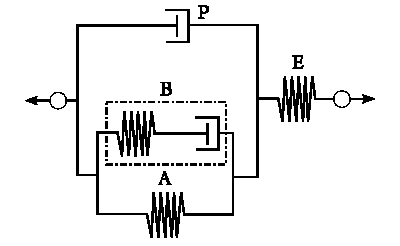
\includegraphics[width=0.6\textwidth]{figures/hybrid_model}
	\caption{Rheological representation of the Hybrid model.}
\label{fig:hybrid_model}
\end{figure}

\section{Based on free energy}

On the other hand, to describe the
deformation rate and temperature dependence of the deformation, a thermodynamics based
viscoplastic constitutive equation and a thermo-mechanically-coupled large-deformation theory have
been proposed (Ghorbel, 2008, Anand, 2009, Srivastava et al., 2010). \cite{uchidaMicroMesoMacroscopic2013}

\colorbox{BrickRed}{See about \cite{anandTheoryAmorphousSolids2003}. And also \cite{ghorbelViscoplasticConstitutiveModel2008,anandThermomechanicallyCoupledTheory2009, amesThermomechanicallyCoupledTheory2009, pouriayevaliConstitutiveDescriptionRatesensitive2013}}

\section{Models considering bulk crystallinity}

The following set of models considers different phases in the semi-crystalline polymers, a crystalline phase and an amorphous phase.
They do so through simple geometric considerations which mostly only include the bulk crystallinity.
The simplest results of this kind are the Voigt and Reuss mixture rules \citep{wardIntroductionMechanicalProperties2004}.
It is assumed that the two phases are disposed as layers, with the Voigt rule obtained assuming that the strain is the same in all composite layers, yielding
\begin{equation}
	\label{eq:voigt_mixture_rule}
	E_\text{mix} = E_A \chi + E_B (1 - \chi),
\end{equation}
for the modulus of the mixture, $E_\text{mix}$, with $E_A$ and $E_B$ the modulus of each phase, and $\chi$ the volume fraction of the phase $A$.
This rule sets an upper limit to the stiffness of the composite material.
If on the other hand, it is assumed that the stress is the same in all composite layers, the modulus found for the mixture is
\begin{equation}
	E_\text{mix} = \frac{E_A E_B}{E_A \chi + E_B (1-\chi)},
\end{equation}
according to the so-called Reuss mixture rule.
This choice corresponds to a lower bound for the stiffnes of the composite material.

Perhaps the work of Takayanagi and coworkers \citep{ takayanagiApplicationEquivalentModel1964} was the first to consider such an approach to model semi-crystalline polymers.
The mixture rule found is neither the Voigt or the Reuss mixture rule, since the phases are not arranged in layers.
Instead the amorphous phase is kept at the corner of the volume element considered, with dimensions $\varphi$ and $\lambda$, as depicted in Figure~\eqref{fig:model_takayanagi}.
The quantity $\varphi \lambda$ is equal to the volume fraction of amorphous polymer, supplying an extra degree of freedom that can be correlated to the distribution of one phase in the other.
A more homegeneous distribution of the phase with the lower volume fraction leads to similar values for $\varphi$ and $\lambda$, while inhomogeneities in either direction favor one or the other parameter.
In \citep{takayanagiMechanicalPropertiesFine1967}, the authors consider employing similar techniques to model drawn samples of polyethylene (PE), isotactic propylene (iPP), among other crystalline polymers.
\begin{figure}
	\centering
	\includegraphics[width=.9\textwidth]{example-image-a}
	\caption{Mixture model of Takayanagi et al. \citep{takayanagiApplicationEquivalentModel1964} for semi-crystalline polymers.}
\label{fig:model_takayanagi}
\end{figure}

G'sell, Dahoun and co-workers \citep{gsellEvolutionMicrostructureSemicrystalline1994, dahounPlasticBehaviorDeformation1995} employ a mixture model using the Voigt composite model to combine the contributions from the amorphous (rubber-like) and the crystalline (viscoplastic) portions of the polymer, assumed to be above the glass transition temperature to describe HDPE and PEEK subject to uniaxial traction and pure shear.
The response of the amorphous portion of the polymer is given according to the rubber elastic model in \citep{wuImprovedNetworkModels1993}, while the behavior of the crystalline phase is modeled following Parks and Ahzi \citep{parksPolycrystallinePlasticDeformation1990}.
It is based on a local-global interaction model established for polycrystalline metal \citep{molinariSelfConsistentApproach1987}, taking into account the kinematically indeterminate component of the stress in a rigid-viscoplastic crystal due the locally inextensible direction.
They consider a fully crystalline HDPE and make predictions regarding the large deformation texture developed, as well as the macroscopic stress-strain response.

% See about \cite{raoStudyStraininducedCrystallization2001}
% The model by Rao et al. \citep{raoStudyStraininducedCrystallization2001}, where the Helmholtz free energy free energy is divided according to the crystallinity, considered as an internal variable.

Ahzi et al. \citep{ahziModelingDeformationBehavior2003} model PET at large strains including strain-induced polymer crystallization, at temperatures above the glass transition temperature.
The model is based on \citep{boyceConstitutiveModelFinite2000}, considering to distinct resistances, an intermolecular and network resistance.
As in the basis model, the network stress, $\pmb\sigma_B$, is given by the Arruda-Boyce eight-chain model (see Equation~\eqref{eq:eigth_chain_model}), and the viscous element follows the Bergström-Boyce model (see Equation~\eqref{eq:bb_reptation_model}).
The intermolecular resistance, however, is treated in a composite framework where the crystalline and amorphous phases are considered as two separate resistances coupled through either a Voigt or a Reuss like mixture rule, which yields an upper bound and lower bound for the stiffness, respectively.
The elastic elements corresponding to the crystalline and amorphous phases follow the Hencky model (see Equation~\eqref{eq:hencky_model}), and the viscous elements a model similar to the one proposed by Argon (see Equation~\eqref{eq:argon_model_free_enthalpy}), where the athermal strength $s_i$ in each phase evolves according to
\begin{equation}
	\dot s = h_i\dot\gamma_i,
\end{equation}
where $h_i$ are the hardening rates.

Regarding the application of the mixture rules in intermolecular resistance, there are contributions coming from the crystalline part, denoted by $c$, and the amorphous part, $a$, of the semi-crystalline polymer.
These are combined according to the degree of crystallinity, $\chi$, in two ways (see Figure~\ref{fig:ahzi_combiniations}):
\begin{itemize}
	\item in parallel, such that the gradient acting in each element is equal and the Cauchy stress is supplied by
	\begin{equation}
		\bm\sigma_A = \chi\bm\sigma_A^c + (1 -\chi)\bm\sigma_A^a.
	\end{equation}
	\item in series, such that the stress acting on both elements is the same and the plastic rate of deformation is given by
	\begin{equation}
		\mathbf D^p_A = \chi \mathbf D^{p,\ c}_A + (1 -\chi)\mathbf D^{p,\ a}_A.
	\end{equation}
\end{itemize}
\begin{figure}
	\centering
	\includegraphics[width=0.9\textwidth]{example-image-a}
	\caption{Mixture models considered by Ahzi et al. \citep{ahziModelingDeformationBehavior2003}.}
\label{fig:ahzi_combiniations}
\end{figure}
The crystallization rate is expressed following a non-isothermal phenomenological expression based on the modified Avrami equation
\begin{equation}
	\dot \chi = \chi_\infty \frac{\dot\varepsilon_\text{eq}}{\dot\varepsilon_\text{ref} } m K_\text{av}(T) (-\ln(1-y))^{(m-1)/m} (1-y)\exp\left(\xi\frac{\operatorname{tr} \bm \sigma}{G_\text{comp}}\right),
\end{equation}
where $\chi_\infty$ is the maximum degree of crystallinity, $m$ is the Avrami, $\xi$ is a dimensionless model parameter, $G_\text{comp}$ is the composite bulk modulus, $\dot \varepsilon_\text{eq}$ is the applied equivalent strain rate and $\dot\varepsilon_\text{ref}$ is taken as the maximum strain rate for which experimental results are available for the calibration of the model parameters.
% See how the strain rate is defined
$K_\text{av}$ is the transformation rate function, which is defined in the case of PET as
\begin{equation}
	K_\text{av}(T) = 1.47\times 10^{-3} \left[\frac{4\pi \mathrm{Nu}}{3\chi_\infty}\right]^{1/3} \exp\left[-\left(\frac{T - 141}{47.33}\right)\right], \quad \text{(\si{\per\second}, $T$ in \si{\celsius})},
\end{equation}
with $\mathrm{Nu}$ the number density of nuclei initially present within the amorphous phase.

Strobl and co-workers \citep{hongModelTreatingTensile2004, hongModelTreatmentTensile2004, naViscousForceDominatedTensileDeformation2006} propose a somewhat similar description for polyethylene.
They also consider essentially two arms in a rheological model (see Figure~\eqref{fig:strobl_model}).
The first is a Maxwell arm with a linear spring and an Eyring dashpot in series.
The second is found through a Voigt mixture rule between a rubber elastic element and an elasto-plastic element.
These choices are supported by extensive experimental results on PEVA and PE.
\begin{figure}
	\centering
	\includegraphics[width=.9\textwidth]{example-image-a}
	\caption{Model proposed by Strobl and co-workers \citep{hongModelTreatingTensile2004, hongModelTreatmentTensile2004, naViscousForceDominatedTensileDeformation2006} for semi-crystalline polymers.}
\label{fig:strobl_model}
\end{figure}

Makradi et al. \citep{makradiTwophaseSelfconsistentModel2005} extend this model considering a self-consistent approach based on the Eshelby result.
 which amount to considering as the intermolecular resistance a Maxwell arms where the stiffness of is an equivalent sitffness and the strain rate is also and equilvaltent.
The stress corresponding to the intermolecular resistance is thus given according to the Hencky model (see Equation~\eqref{eq:hencky_model}) with the isotropic elastic moduli $\bm{\mathsf D}$ is given according to a self-consistente method proposed by Hill \citep{hillSelfconsistentMechanicsComposite1965} and Budiansky \citep{Budiansky}.
The flow rule for the viscous element is given by Equation~\eqref{eq:flow_rule_directions}, neglecting the volumetric part.
The strain rate, $\dot \gamma_\text{dev}$ defined as an average shear rate, $\dot{\bar\gamma}$ according to
\begin{equation}
	\label{eq:def_avg_strain_rate}
	\dot{\bar\gamma} = \frac{1}{V}\int_V \dot \gamma\ dV = \frac{1}{V}\sum_i V_i \dot{\gamma}_i,
\end{equation}
where
\begin{equation}
	\dot \gamma_i = \frac{1}{V_i}\int_{V_i} \dot \gamma\ dV_i,
\end{equation}
with $V_i$ the volume of the $i$th phase and $V$ representing the total volume.
For each phase, the flow rule is also given by Equation~\eqref{eq:flow_rule_directions}, neglecting the volumetric part, with the strain rate in each phase following a power law (see Equation~\eqref{eq:flow_rule_power_law}).
Thus, the average strain rate follows a power law too with an average strength $\bar s$.
It can be shown, taking into account Eshelby's results for an ellipsoidal inclusion, that
\begin{equation}
	\frac{\dot \gamma_i}{\dot{\bar \gamma}} = \frac{5}{3} - \frac{2}{3}\frac{s_i}{\bar s} \left(\frac{\dot \gamma_i}{\dot{\bar \gamma}}\right)^{1/n},
\end{equation}
which combined with Equation~\eqref{eq:def_avg_strain_rate} and the corresponding power law, yields the average strain rate.
The authors employ the same description for the evolution of the crystallinity as \cite{ahziModelingDeformationBehavior2003}, in addition to the Flory’s theory to predict the onset of crystallization as a function of the processing temperature and the extension of the polymer molecules.
Later Regrain et al. \citep{regrainMultimechanismModelsSemicrystalline2009} extend the DID models to semi-crystalline models also employing a self-consistent scheme to consider the contribution of both phases.

Dusunceli et al. \citep{dusunceliModellingEffectsDegree2008} extends the viscoplasticity theory based on overstress (VBO) to include crystallinity.
This is achieved describing both phases employing the VBO model and considering their contributions employing either a Voigt or a Reuss mixture rule.
The authors validate their model employing both polyethylenes (UHWPE and XLPE) and PTFE.

Ayoub et al. \citep{ayoubModellingLargeDeformation2010, ayoubEffectsCrystalContent2011} present a model very similar to \cite{ahziModelingDeformationBehavior2003} and \cite{boyceConstitutiveModelFinite2000} to describe the mechanical behavior of HDPE.
The inelastic mechanisms involve two parallel elements: a visco-hyperelastic network resistance acting in parallel with a viscoelastic–viscoplastic intermolecular resistance where the amorphous and crystalline phases are explicitly taken into consideration.
The semi-crystalline polymer is considered as a two-phase composite in a way similar to what has already been described.
\colorbox{BrickRed}{Add the difference with exponent and the try to capture PE and comparison with different HDPE, LDPE, ULPE}
A similar model can be found in \citep{abdul-hameedTwophaseHyperelasticviscoplasticConstitutive2014}, where the major difference is the arrangment of the mechanical elements in the rheological model.
Very recently, Cundiff et al. \citep{cundiffModelingViscoplasticBehavior2022} propose another model where the inclusion of the crystallinity is achieved in the same way.
Regarding the the constitutive description of each phase it employs much of the same laws found in \cite{ahziModelingDeformationBehavior2003} and \cite{chowdhuryEffectsManufacturingInducedVoids2008}, already described.

Lastly, the two-phase model of Cangemi and Meimon for semi-crystalline polymers \citep{cangemiTwoPhaseModelMechanical2001} achieves the inclusion of the bulk crystallinity into the description of a semi-crystalline polymer in a different way.
It is based on the continuum mixture theory such that according to the microstructure of semi-crystalline polymers, the free amorphous phase is assumed comparable to a fluid which saturates the complementary space to that of the solid structure, the crystalline phase plus the rigid amorphous phase.

\section{Micromechanical models}

The last set of models includes in addition to the bulk crystallinity some geometric considerations at the micro scale.
Accordingly, a micromechanical modeling based on the laminar composite approach was proposed by Lee et al. \citep{leeMicromechanicalModelingLarge1993, leeSimulationLargeStrain1993}.
In this model, rigid-viscoplastic amorphous phase using 8-chain model (see Equation~\eqref{eq:eigth_chain_model}) was added, and Sachs/Taylor hybrid interaction law was used to relate the mechanical properties of microscopic two-phase inclusion and an aggregation of the inclusions.
In these models, a crystalline polymer is regarded as a polycrystalline aggregate of randomly distributed crystallites which plastically deform in a co-operative manner.
It does not consider the mesoscopic structure of the polymer.

According to Uchida et al. \citep{uchidaMicroMesoMacroscopic2013}, these models were then improved to more realistic elasto-viscoplastic models by Nikolov et al. \citep{nikolovMicroMacroConstitutive2000, nikolovMultiscaleConstitutiveModeling2002, niko2006} and van Dommelene et al. \citep{vandommelenMicromechanicalModelingElastoviscoplastic2003}
In a similar vein, Guan et al. \citep{guanMicromechanicalModelElastic2004} present a micromechanical analysis of the elastic properties of semicrystalline thermoplastic materials.

Bedoui et al. \citep{bedouiMicromechanicalModelingIsotropic2006} considers a micromechanical model applied to infinitesimal strain, concluding that the spherulitic mesostructure does not affect the response of the material at that level of strain.
The phase of the amorphous part of the semi-crystalline polymers has a noticeable impact on the stiffness of the polymer.
There is a moderate agreement between the predictions and the experimental results.

Alternatively, Uchida and coworkers \citep{uchidaMicroMesoMacroscopic2013} developed a large deformation finite element homogenization model of spherulite of HDPE.
This in contrast to the previously described models, because interaction laws applied in these models have no geometric information, compatibility and equilibrium in the spherulite cannot be taken into consideration.
Since this model directly solves both of microscopic and mesoscopic displacement fields using FE-based homogenization scheme, compatibility and equilibrium between adjacent microstructure in the spherulite are automatically satisfied.
According to the authors, when macroscopic response and texture evolution are required, the former micromechanical-based model are suitable.
Meanwhile, homogenization-based model is proper when distributions of strain and stress in the spherulite are required.
Regarding the size of the representative domain, Teixeira-Pinto et al. \citep{teixeira-pintoSizeEstimationRepresentative2016} claim that it significantly exceeds the size of a single spherulite.


% \colorbox{BrickRed}{Consider saying something about deformation maps \cite{frostDeformationmechanismMapsPlasticity1982}, \cite{odonnellComputerProgramGenerating1991} \cite{kawasakiManyFacetsDeformation2013, vanloockDeformationFailureMaps2018, richardPredictingPlasticityDisordered2020}}

\chapter{Conclusion and Future Works} \label{ch:conclusions}

This work has two goals: first, it focuses on computational techniques for numerical simulation of thermomechanical problems and, more broadly, multi-physics problems; second, it attempts to provide an overview of the state-of-the-art in semi-crystalline polymer constitutive modeling.
They are both critical to the creation of a robust computational toolbox for the design and optimization of semi-crystaline polymer based materials as well as the simulation of their thermomechanical behavior under mechanical and thermal loadings.

The first task requires both a thermodynamically consistent description of continuum thermodynamics and a precise formulation of the thermomechanical problem.
A thorough investigation of the available approaches to solving coupled problems is provided, with a particular focus on thermomechanical problems.
The strongly coupled or implicit partitioned schemes are chosen as the most promising approach because they can take advantage of existing software, provide accurate results that agree with a monolithic approach, are not memory intensive, are easy to implement, and are competitive in terms of computational efficiency through the use of convergence acceleration techniques.
Recasting the problem as a system of nonlinear equations, where the residual is the difference between the initial input and its output after applying the fixed-point corresponding to the isothermal split, allows the straightforward use of a wide selection of methods for the solution of systems of nonlinear equations.
This approach is applied specifically to the thermomechanical problem here, but it applies to other multi-physics phenomena with little modification.
These are the fixed-point method, the underrelaxation method, the Aitken relaxation, the Broyden-like family of methods, the Newton-Krylov methods, and the polynomial vector extrapolation methods MPE and RRE in cycling mode.

The validation of the thermomechanical solver and the implicit solution methods, as well as their comparison, is performed by considering an example taken from the literature: the necking of a circular thermoelastoplastic bar.
The numerical results agree with the references, hence supporting the developed solution scheme.
Regarding the comparison of the different implicit techniques, the best performing are the Broyden-like methods with \(\beta=-1\), Type I update, and \(s=1\), corresponding to the good Broyden method, and \(s=2\).
These are both computationally efficient (few calls to the residual function) and memory efficient.
The Aitken relaxation, the simplest and least memory-intensive, also performs well.
The other methods considered, including the Newton-GMRES and the MPE in cycling mode, display worse performance.
Moreover, it has been determined that the most computationally demanding portion of the implicit partitioned schemes is the solution of the mechanical and thermal problems, with the manipulation concerning solely the coupling solver taking a very small part of the total computational time.

The second topic addressed in this work is the constitutive description of semi-crystalline polymers.
To accomplish this, a detailed account of the thermomechanical behavior of semi-crystalline polymers is provided so that the appropriate modeling goals can be established.
It is primarily based on this class of materials' response to various mechanical experiments, ranging from constant strain rate experiments to stress relaxation, creep, and dynamical mechanical analysis.
Semi-crystalline polymers, in constant strain rate experiments, typically exhibit a response that consists of a linear stress-strain relationship followed by yield.
A steady state is sometimes observed, followed by intense strain hardening at large strains.
Regarding the influence of temperature on the behavior of this class of polymers, its increase leads to lower stiffness and yield strength.
However, unlike glassy polymers, they retain usable structural properties even after the glass transition temperature is crossed.
Common semi-crystalline polymers employed in commodity uses are HDPE and PP, while PA, PET, PPA, and PEEK satisfy the requirements of increasingly demanding engineering applications.
The strain rate and the pressure exert the opposite effect on the stiffness and strength of semi-crystalline polymers.
Furthermore, the yield phenomenon in semi-crystalline polymers is neither rate-independent nor linear with the strain rate, requiring appropriate nonlinear modeling.

Concerning the influence of bulk crystallinity and lamellar thickness, an increase in the former implies a nonlinear increase in stiffness and strength, whereas an increase in the latter results in a linear increase in strength for moderate thicknesses, but stagnates for thicker lamella.
Semi-crystalline polymers also have a double yield, which means that, as the strain increases, there are two distinct yield stresses.
This phenomenon is also linked to the temperature softening phenomenon, in which higher strain rates result in significant heat production and temperature increases, causing the material to soften.
Furthermore, cold drawing is common, as when a neck develops in a tensile uniaxial test, where the specimen thins in that region until the natural draw ratio is achieved.
After that, the material in the neck has hardened sufficiently so that the thinned region travels across the specimen rather than decreasing until failure.
Semi-crystalline strain hardening behavior is also similar to rubber elasticity.

In terms of the semi-crystalline polymer response to dynamical mechanical analysis, polymers with high crystallinity do not show a significant drop in storage modulus as frequency decreases in isothermal results.
When the degree of crystallinity is low, a clear viscoelastic transition from glassy to leathery is observed.
In isochronal results, one can observe the various relaxations present in semi-crystalline polymers.
Relaxation I is visible at all crystallinity levels at lower temperatures, while relaxation II and III are more easily detectable at lower and higher crystallinities, respectively.

Finally, the thermal properties of semi-crystalline polymers are similar to those of other polymers in that they have a relatively large linear expansion coefficient and low thermal conductivity and diffusivity.
This raises concerns about heat distortion when using semi-crystalline polymers in engineering applications and difficulties in tuning some manufacturing processes.
On the other hand, they display a desirable behavior when it comes to thermal shocks, despite the large linear thermal expansion coefficient, due to the relatively low Young modulus.
\enlargethispage{\baselineskip}

Given these goals for thermomechanical modeling, an extensive overview of the state-of-the-art in semi-crystalline polymer modeling is provided.
Thermoviscoelasticity is taken as the starting point.
It is, nevertheless, not suitable due to nonlinear features in the behavior of semi-crystalline polymers and its description employing infinitesimal strains.
Finite linear viscoelasticity is a generalization of linear viscoelasticity to large strains, although it does not provide a nonlinear description of semi-crystalline polymers.
Single integral models are yet another approach that attempts to generalize the convolution integral description obtained from infinitesimal viscoelasticity.
It is, however, not adequate for the computation framework based on the FEM method adopted here.

The most common approach is the use of rheological models with appropriate nonlinear viscous and elastic elements.
Within the many possible arrangements of elastic and viscous elements, the generalization of the standard linear solid appears to be the most popular, as employed in the early model of Haward and Thackray \citep{hawardUseMathematicalModel1968} and its generalization by Boyce, Park, and Ahzi \citep{boyceLargeInelasticDeformation1988}.
The viscous element employed in both models is based on Eyring's model for thermally activated processes.
Within that model, an athermal strength controls the yield stress of the polymer, which can be taken as an internal variable in order to capture strain softening behavior \citep{boyceLargeInelasticDeformation1988}, or even the double yield phenomenon \citep{haoUnifiedAmorphousCrystalline2022}.
These two elements, when combined with an Hencky model for the elastic element, are responsible for modeling the pre-yield and yield behavior, which contribute to what is commonly referred to as the intermolecular resistance.
The strain hardening is captured most often through the use of a rubber-elasticity model, such as the Arruda-Bouce eight-chain model \citep{arrudaEffectsStrainRate1995} or the Edward-Vilgis model \citep{edwardsEffectEntanglementsRubber1986} in the so-called network resistance.
Sometimes, the viscous element proposed by Bergstrom-Boyce based on reptation \citep{bergstromConstitutiveModelingLarge1998, bergstromConstitutiveModelingTimedependent2001} is also included in this resistance.
That said, the numerical results presented here support the conclusion that the most recent models for thermoplastics such as the model in \cite{haoUnifiedAmorphousCrystalline2022} are able to effectively capture the behavior of semi-crystalline polymers.

In order to include the bulk crystallinity in the description of semi-crystalline polymers, the most common approach is to model the resistance due to each phase using a thermoplastic model, such as those already mentioned.
Their contributions are then weighted using a mixture rule, such as the Reuss or Voig mixture rules.
This set of models is especially compelling because it allows for the description of a polymer at various degrees of crystallinity using a single set of material parameters.
An interesting suggestion that models well the pre-yield and yield behavior of a semicrystalline polymer is the nonlinear Voigt mixture rule proposed in \cite{ayoubEffectsCrystalContent2011}.
However, The authors only use this strategy for the intermolecular resistance, using different material parameters at each crystallinity level for the network resistance.
In \cite{abdul-hameedTwophaseHyperelasticviscoplasticConstitutive2014}, the network resistance is also modeled including crystalline and amorphous phases, and by employing the same modified Voigt rule.
Models such as those in \cite{ahziModelingDeformationBehavior2003, makradiTwophaseSelfconsistentModel2005} and \cite{cundiffModelingViscoplasticBehavior2022} also try to model the increase in cyrstallinity with strain in polymers such as PET.
Nevertheless, scrutinizing the numerical results provided here for the model in \citep{abdul-hameedTwophaseHyperelasticviscoplasticConstitutive2014} the ability of said model to achieve this goal is limited when it comes to the description of the strain hardening behavior of semi-crystalline polymers that succeds yield. \colorbox{BrickRed}{See this!}
\enlargethispage{\baselineskip}
\section{Future research and challenges}

Building on the research efforts already made in this work to establish a robust computational toolbox for the design of multi-functional semi-crystalline polymers in engineering applications, the author's PhD thesis will address the following challenges:

\begin{itemize}
  \item More physical phenomena will be incorporated into the description of semi-crystalline polymers.
  Electrical, magnetic, and hygromechanical phenomena are examples of such phenomena, which are critical in simulating some manufacturing processes and life service conditions.
  \item Another avenue of research to be explored, is the development of new macroscopic constitutive laws capable of accurately capturing the homogenized response of semi-crystalline polymers.
  In particular, models similar to those of \cite{abdul-hameedTwophaseHyperelasticviscoplasticConstitutive2014} and \cite{ayoubEffectsCrystalContent2011}, where bulk crystallinity is introduced and the material is characterized by the same material parameters with varying degrees of crystallintiy.
  The main challenge is to make an appropriate generalization with the degree of crystallinity of the strain hardening response as understood from the numerical results reviewed in this work.
  In tandem, a thorough investigation of the thermomechanical behavior of the various models available, as well as a detailed validation using various mechanical loading and thermal regimes.
  \item Design of semi-crystalline polymer blends, such as nylon 6/PTFE blends, to provide optimal structural efficiency, manufacturability, and multi-functionality.
  Multi-scale approaches, which transfer information between scales, can provide a more detailed physical understanding of their behavior and the ability to tailor new materials by manipulating their microstructure.
  \item  The modeling and design multi-functional semicrystalline polymeric materials by combining multi-scale strategies with machine learning is to be pursued.
  The work will initially focus on the mechanical response by finding optimal solutions for strength and toughness.
  Later on, the coupling between the mechanical, electro, and transport fields will be addressed enabling the design of advanced multi-functional semicrystalline polymeric materials.

\end{itemize}

\appendix
% \include{annex}

\bibliography{semi_crystalline_polymer.bib}

\end{document}
